\documentclass{article}

% packages
  % basic stuff for rendering math
  \usepackage[letterpaper, top=1in, bottom=1in, left=1in, right=1in]{geometry}
  \usepackage[utf8]{inputenc}
  \usepackage[english]{babel}
  \usepackage{amsmath} 
  \usepackage{amssymb}
  % \usepackage{amsthm}

  % extra math symbols and utilities
  \usepackage{mathtools}        % for extra stuff like \coloneqq
  \usepackage{mathrsfs}         % for extra stuff like \mathsrc{}
  \usepackage{centernot}        % for the centernot arrow 
  \usepackage{bm}               % for better boldsymbol/mathbf 
  \usepackage{enumitem}         % better control over enumerate, itemize
  \usepackage{hyperref}         % for hypertext linking
  \usepackage{fancyvrb}          % for better verbatim environments
  \usepackage{newverbs}         % for texttt{}
  \usepackage{xcolor}           % for colored text 
  \usepackage{listings}         % to include code
  \usepackage{lstautogobble}    % helper package for code
  \usepackage{parcolumns}       % for side by side columns for two column code
  \usepackage{array} 

  % page layout
  \usepackage{fancyhdr}         % for headers and footers 
  \usepackage{lastpage}         % to include last page number in footer 
  \usepackage{parskip}          % for no indentation and space between paragraphs    
  \usepackage[T1]{fontenc}      % to include \textbackslash
  \usepackage{footnote}
  \usepackage{etoolbox}
  \usepackage[table]{xcolor}

  % for custom environments
  \usepackage{tcolorbox}        % for better colored boxes in custom environments
  \tcbuselibrary{breakable}     % to allow tcolorboxes to break across pages

  % figures
  \usepackage{pgfplots}
  \pgfplotsset{compat=1.18}
  \usepackage{float}            % for [H] figure placement
  \usepackage{tikz}
  \usepackage{tikz-cd}
  \usepackage{circuitikz}
  \usetikzlibrary{shapes,arrows,positioning}
  \usetikzlibrary{arrows}
  \usetikzlibrary{positioning}
  \usetikzlibrary{calc}
  \usepackage{graphicx}
  \usepackage{caption} 
  \usepackage{subcaption}
  \captionsetup{font=small}

  % for tabular stuff 
  \usepackage{dcolumn}

  \usepackage[nottoc]{tocbibind}
  \pdfsuppresswarningpagegroup=1
  \hfuzz=5.002pt                % ignore overfull hbox badness warnings below this limit

% New and replaced operators
  \DeclareMathOperator{\Tr}{Tr}
  \DeclareMathOperator{\Sym}{Sym}
  \DeclareMathOperator{\Span}{span}
  \DeclareMathOperator{\std}{std}
  \DeclareMathOperator{\Cov}{Cov}
  \DeclareMathOperator{\Var}{Var}
  \DeclareMathOperator{\Corr}{Corr}
  \DeclareMathOperator{\pos}{pos}
  \DeclareMathOperator*{\argmin}{\arg\!\min}
  \DeclareMathOperator*{\argmax}{\arg\!\max}
  \newcommand{\ket}[1]{\ensuremath{\left|#1\right\rangle}}
  \newcommand{\bra}[1]{\ensuremath{\left\langle#1\right|}}
  \newcommand{\braket}[2]{\langle #1 | #2 \rangle}
  \newcommand{\qed}{\hfill$\blacksquare$}     % I like QED squares to be black
  \def\ojoin{\setbox0=\hbox{$\bowtie$}%
    \rule[-.02ex]{.25em}{.4pt}\llap{\rule[\ht0]{.25em}{.4pt}}}
  \def\lojoin{\mathbin{\ojoin\mkern-5.8mu\bowtie}}
  \def\rojoin{\mathbin{\bowtie\mkern-5.8mu\ojoin}}
  \def\fojoin{\mathbin{\ojoin\mkern-5.8mu\bowtie\mkern-5.8mu\ojoin}}
% Custom Environments
  \newtcolorbox[auto counter, number within=section]{question}[1][]
  {
    colframe = orange!25,
    colback  = orange!10,
    coltitle = orange!20!black,  
    breakable, 
    title = \textbf{Question \thetcbcounter ~(#1)}
  }

  \newtcolorbox[auto counter, number within=section]{exercise}[1][]
  {
    colframe = teal!25,
    colback  = teal!10,
    coltitle = teal!20!black,  
    breakable, 
    title = \textbf{Exercise \thetcbcounter ~(#1)}
  }
  \newtcolorbox[auto counter, number within=section]{solution}[1][]
  {
    colframe = violet!25,
    colback  = violet!10,
    coltitle = violet!20!black,  
    breakable, 
    title = \textbf{Solution \thetcbcounter}
  }
  \newtcolorbox[auto counter, number within=section]{lemma}[1][]
  {
    colframe = red!25,
    colback  = red!10,
    coltitle = red!20!black,  
    breakable, 
    title = \textbf{Lemma \thetcbcounter ~(#1)}
  }
  \newtcolorbox[auto counter, number within=section]{theorem}[1][]
  {
    colframe = red!25,
    colback  = red!10,
    coltitle = red!20!black,  
    breakable, 
    title = \textbf{Theorem \thetcbcounter ~(#1)}
  } 
  \newtcolorbox[auto counter, number within=section]{proposition}[1][]
  {
    colframe = red!25,
    colback  = red!10,
    coltitle = red!20!black,  
    breakable, 
    title = \textbf{Proposition \thetcbcounter ~(#1)}
  } 
  \newtcolorbox[auto counter, number within=section]{corollary}[1][]
  {
    colframe = red!25,
    colback  = red!10,
    coltitle = red!20!black,  
    breakable, 
    title = \textbf{Corollary \thetcbcounter ~(#1)}
  } 
  \newtcolorbox[auto counter, number within=section]{proof}[1][]
  {
    colframe = orange!25,
    colback  = orange!10,
    coltitle = orange!20!black,  
    breakable, 
    title = \textbf{Proof. }
  } 
  \newtcolorbox[auto counter, number within=section]{definition}[1][]
  {
    colframe = yellow!25,
    colback  = yellow!10,
    coltitle = yellow!20!black,  
    breakable, 
    title = \textbf{Definition \thetcbcounter ~(#1)}
  } 
  \newtcolorbox[auto counter, number within=section]{example}[1][]
  {
    colframe = blue!25,
    colback  = blue!10,
    coltitle = blue!20!black,  
    breakable, 
    title = \textbf{Example \thetcbcounter ~(#1)}
  } 
  \newtcolorbox[auto counter, number within=section]{algo}[1][]
  {
    colframe = green!25,
    colback  = green!10,
    coltitle = green!20!black,  
    breakable, 
    title = \textbf{Algorithm \thetcbcounter ~(#1)}
  } 

  \BeforeBeginEnvironment{example}{\savenotes}
  \AfterEndEnvironment{example}{\spewnotes}
  \BeforeBeginEnvironment{lemma}{\savenotes}
  \AfterEndEnvironment{lemma}{\spewnotes}
  \BeforeBeginEnvironment{theorem}{\savenotes}
  \AfterEndEnvironment{theorem}{\spewnotes}
  \BeforeBeginEnvironment{corollary}{\savenotes}
  \AfterEndEnvironment{corollary}{\spewnotes}
  \BeforeBeginEnvironment{proposition}{\savenotes}
  \AfterEndEnvironment{proposition}{\spewnotes}
  \BeforeBeginEnvironment{definition}{\savenotes}
  \AfterEndEnvironment{definition}{\spewnotes}
  \BeforeBeginEnvironment{exercise}{\savenotes}
  \AfterEndEnvironment{exercise}{\spewnotes}
  \BeforeBeginEnvironment{proof}{\savenotes}
  \AfterEndEnvironment{proof}{\spewnotes}
  \BeforeBeginEnvironment{solution}{\savenotes}
  \AfterEndEnvironment{solution}{\spewnotes}
  \BeforeBeginEnvironment{question}{\savenotes}
  \AfterEndEnvironment{question}{\spewnotes}
  \BeforeBeginEnvironment{code}{\savenotes}
  \AfterEndEnvironment{code}{\spewnotes}

  \definecolor{dkgreen}{rgb}{0,0.6,0}
  \definecolor{gray}{rgb}{0.5,0.5,0.5}
  \definecolor{mauve}{rgb}{0.58,0,0.82}
  \definecolor{lightgray}{gray}{0.93}

  % default options for listings (for code)
  \lstset{
    autogobble,
    frame=ltbr,
    language=SQL,                           % the language of the code
    aboveskip=3mm,
    belowskip=3mm,
    showstringspaces=false,
    columns=fullflexible,
    keepspaces=true,
    basicstyle={\small\ttfamily},
    numbers=left,
    firstnumber=1,                        % start line number at 1
    numberstyle=\tiny\color{gray},
    keywordstyle=\color{blue},
    commentstyle=\color{dkgreen},
    stringstyle=\color{mauve},
    backgroundcolor=\color{lightgray}, 
    breaklines=true,                      % break lines
    breakatwhitespace=true,
    tabsize=3, 
    xleftmargin=2em, 
    framexleftmargin=1.5em, 
    stepnumber=1
  }

% Page style
  \pagestyle{fancy}
  \fancyhead[L]{Databases}
  \fancyhead[C]{Muchang Bahng}
  \fancyhead[R]{Fall 2024} 
  \fancyfoot[C]{\thepage / \pageref{LastPage}}
  \renewcommand{\footrulewidth}{0.4pt}          % the footer line should be 0.4pt wide
  \renewcommand{\thispagestyle}[1]{}  % needed to include headers in title page

\begin{document}

\title{Databases}
\author{Muchang Bahng}
\date{Fall 2024}

\maketitle
\tableofcontents
\pagebreak 

  This is a course on database languages (SQL), database systems (Postgres, SQL server, Oracle, MongoDB), and data analysis. 

  \begin{definition}[Data Model]
    A \textbf{data model} is a notation for describing data or information, consisting of 3 parts. 
    \begin{enumerate}
      \item \textit{Structure of the data}. The physical structure (e.g. arrays are contiguous bytes of memory or hashmaps use hashing). This is higher level than simple data structures. 
      \item \textit{Operations on the data}. Usually anything that can be programmed, such as \textbf{querying} (operations that retrieve information), \textbf{modifying} (changing the database), or \textbf{adding/deleting}. 
      \item \textit{Constraints on the data}. Describing what the limitations on the data can be. 
    \end{enumerate}
  \end{definition}

  There are two general types: relational databases, which are like tables, and semi-structured data models, which follow more of a tree or graph structure (e.g. JSON, XML).  

\section{Relational Algebra}

  The most intuitive way to store data is with a \textit{table}, which is called a relational data model, which is the norm since the 1990s. 

  \begin{definition}[Relational Data Model]
    A \textbf{relational data model} is a data model where its structure consists of 
    \begin{enumerate}
      \item \textbf{relations}, which are two-dimensional tables. 
      \item Each relation has a set of \textbf{attributes}, or columns, which consists of a name and the data type (e.g. int, float, string, which must be primitive).\footnote{The attribute type cannot be a nonprimitive type, such as a list or a set. }
      \item Each relation is a set\footnote{Note that since this is a set, the ordering of the rows doesn't matter , even though the output is always in some order.} of \textbf{tuples} (rows), which each tuple having a value for each attribute of the relation. Duplicate (agreeing on all attributes) tuples are not allowed. 
    \end{enumerate}
    So really, relations are tables, tuples are rows, attributes are columns. 
  \end{definition}

  \begin{definition}[Schema]
    The \textbf{schema} of a relational database just describes the form of the database, with the name of the database followed by the attributes and its types. 
    \begin{lstlisting}
      Beer (name string, brewer string)
      Serves (bar string, price float)
      ...
    \end{lstlisting}
  \end{definition}

  \begin{definition}[Instance]
    The entire set of tuples for a relation is called an \textbf{instance} of that relation. If a database only keeps track of the instance now, the instance is called the \textbf{current instance}, and \textbf{temporal databases} also keep track of the history of its instances. 
  \end{definition}

  SQL (Structured Query Language) is the standard query language supported by most DBMS. It is \textbf{declarative}, where the programmer specifies what answers a query should return,but not how the query should be executed. The DBMS picks the best execution strategy based on availability of indices, data/workload characteristics, etc. (i.e. provides physical data independence). It contrasts to a \textbf{procedural} or an \textbf{operational} language like C++ or Python. One thing to note is that keywords are usually written in uppercase by convention. 

  \begin{definition}[Primitive Types]
    The primitive types are listed. 
    \begin{enumerate}
      \item \textit{Characters}. \texttt{CHAR(n)} represents a string of fixed length $n$, where shorter strings are padded, and \texttt{VARCHAR(n)} is a string of variable length up to $n$, where an endmarker or string-length is used. 
      \item \textit{Bit Strings}. \texttt{BIT(n)} represents bit strings of length $n$. \texttt{BIT VARYING(n)} represents variable length bit strings up to length $n$. 
      \item \textit{Booleans}. \texttt{BOOLEAN} represents a boolean, which can be \texttt{TRUE}, \texttt{FALSE}, or \texttt{UNKNOWN}. 
      \item \textit{Integers}. \texttt{INT} or \texttt{INTEGER} represents an integer. 
      \item \textit{Floating points}. \texttt{FLOAT} or \texttt{REAL} represents a floating point number, with a higher precision obtained by \texttt{DOUBLE PRECISION}. 
      \item \textit{Datetimes}. \texttt{DATE} types are of form \texttt{'YYYY-MM-DD'}, and \texttt{TIME} types are of form \texttt{'HH:MM:SS.AAAA'} on a 24-hour clock. 
    \end{enumerate}
  \end{definition}

  \subsection{Tables, Attributes, and Keys}

    Before we can even query or modify relations, we should know how to make or delete one. 

    \begin{theorem}[\texttt{CREATE TABLE}, \texttt{DROP TABLE}]
      We can create and delete a relation using \texttt{CREATE TABLE} and \texttt{DROP TABLE} keywords and inputting the schema. 
      \begin{lstlisting}
        CREATE TABLE Movies(
          name CHAR(30), 
          year INT, 
          director VARCHAR(50), 
          seen DATE
        ); 

        DROP TABLE Movies; 
      \end{lstlisting}
    \end{theorem}

    What if we want to add or delete another attribute? This is quite a major change. 

    \begin{theorem}[\texttt{ALTER TABLE}]
      We can add or drop attributes by using the \texttt{ALTER TABLE} keyword followed by 
      \begin{enumerate}
        \item \texttt{ADD} and then the attribute name and then its type. 
        \item \texttt{DROP} and then the attribute name. 
      \end{enumerate}
      \begin{lstlisting}
        ALTER TABLE Movies ADD rating INT; 
        ALTER TABLE Movies DROP director; 
      \end{lstlisting}
    \end{theorem}

    \begin{theorem}[\texttt{DEFAULT}]
      We can also determine default values of each attribute with the \texttt{DEFAULT KEYWORD}. 
      \begin{lstlisting}
        ALTER TABLE Movies ADD rating INT 0; 
        ...
        CREATE TABLE Movies(
          name CHAR(30) DEFAULT 'UNKNOWN', 
          year INT DEFAULT 0, 
          director VARCHAR(50), 
          seen DATE DEFAULT '0000-00-00'
        ); 
      \end{lstlisting}
      
    \end{theorem}

    \begin{definition}[Key]
      A set of attributes $\mathcal{K}$ form a \textbf{key} for a relation 
      \begin{enumerate}
        \item if we do not allow two tuples in any relation instance to have the same values in \textit{all} attributes of the key (i.e. in general). 
        \item no proper subset of $\mathcal{K}$ can also be a key for \textit{any} relation instance, that is, $\mathcal{K}$ is \textit{minimal}.\footnote{By minimal we do not mean that the number of attributes in $K$ is minimal. It is minimal in the sense that no proper subset of $\mathcal{K}$ can be a key.}
      \end{enumerate}
      A relation may have multiple keys, but we typically pick one as the \textbf{primary key} and underline all its attributes in the schema, e.g. Address(\underline{street}, city, state, \underline{zip}). 
    \end{definition}

    While we can make a key with a set of attributes, many databases use artificial keys such as unique ID numbers for safety. 

    \begin{example}[Keys of User Relation]
      Given the schema \textit{User(uid, name, age)}, 
      \begin{enumerate}
        \item \textit{uid} is a key of \textit{User} 
        \item \textit{age} is not a key (not an identifier) even if the relation at the current moment all have different ages. 
        \item \{\textit{uid, name}\} is not a key (not minimal)
      \end{enumerate}
    \end{example}

  \subsection{Relational Algebra}

    We've talked about the structure of the data model, but we still have to talk about operations and constraints. We will focus on the operations here, which can be introduced with \textit{relational algebra}, which gives a powerful way to construct new relations from given relations. Really, SQL is a syntactically sugared form of relational algebra. 

    The reason we need this specific query language dependent on relational algebra is that it is \textit{less} powerful than general purpose languages like C or Python. These things can all be stored in structs or arrays, but the simplicity allows the compiler to make huge efficiency improvements. 

    An algebra is really just an algebraic structure with a set of operands (elements) and operators.  

    \begin{definition}[Relational Algebra]
      A relational algebra consists of the following operands. 
      \begin{enumerate}
        \item Relations $R$, with attributes $A_i$. 
        \item Operations. 
      \end{enumerate}
      It has the following operations. 
      \begin{enumerate}
        \item \textit{Set Operations}. Union, intersection, and difference. 
        \item \textit{Removing}. Selection removes tuples and projection removes attributes. 
        \item \textit{Combining}. Cartesian products, join operations. 
        \item \textit{Renaming}. Doesn't affect the tuples, but changes the name of the attributes or the relation itself. 
      \end{enumerate}
    \end{definition}

    Let's take a look at each of these operations more carefully, using the following relation. 

    \begin{figure}[H]
      \centering
      \begin{tabular}{|l|l|r|}
      \hline
      \rowcolor[HTML]{E26B0A} 
      \textcolor{white}{\textbf{bar}} & \textcolor{white}{\textbf{beer}} & \textcolor{white}{\textbf{price}} \\ \hline
      \rowcolor[HTML]{FBCEB1}
      The Edge & Budweiser & 2.50 \\ \hline
      \rowcolor[HTML]{FBCEB1}
      The Edge & Corona & 3.00 \\ \hline
      \rowcolor[HTML]{FBCEB1}
      Satisfaction & Budweiser & 2.25 \\ \hline
      \end{tabular}
      \caption{The example relation, which we will denote \texttt{serves}, which we will use to demonstrate the following operations.} 
      \label{fig:serves}
    \end{figure}
    
    \begin{definition}[Set Operations]
      Given relations $R$ and $S$ which must have the same schema (if not, just apply a projection), we can do the following set operations. 
      \begin{enumerate}
        \item Union. $R \cup S$. 
        \item Intersection. $R \cap S$, which can be written also as $R - (R - S), S - (S - R)$, and surprisngly $R \bowtie S$.\footnote{The natural join will check for all attributes in each schema, but sine we assumed that they had the same schema, it must check for equality over all attributes.}
        \item Difference. $R - S$. 
      \end{enumerate}
      This is implemented as the \texttt{UNION}, \texttt{EXCEPT}, \texttt{INTERSECT} operations in SQL. Given that 
      \begin{enumerate}
        \item $\mathrm{Bag1} = \{1, 2, 3\}$
        \item $\mathrm{Bag2} = \{2, 3, 4\}$
      \end{enumerate}
      We have 
      \begin{lstlisting}
        (SELECT * FROM Bag1) 
        UNION 
        (SELECT * FROM Bag2);     // {1, 2, 3, 4}

        (SELECT * FROM Bag1) 
        EXCEPT 
        (SELECT * FROM Bag2);     // {1} 

        (SELECT * FROM Bag1) 
        INTERSECT 
        (SELECT * FROM Bag2);     // {2, 3}
      \end{lstlisting}
    \end{definition}

    \begin{definition}[Selection]
      The \textbf{selection} operator $\sigma_p$ filters the tuples of a relation $R$ by some condition $p$. It must be the case that $p$ is deducible by looking only at that row. 
      \begin{equation}
        \sigma_p R
      \end{equation}
      This is analogous to the \texttt{WHERE} keyword. 
      \begin{lstlisting}
        SELECT * 
        FROM relation 
        WHERE 
          p_1 AND p_2 AND ... ; 
      \end{lstlisting}
    \end{definition}

    This also allows us to define the in and not in keywords. 

    \begin{definition}[\texttt{IN} and \texttt{NOT IN}]
      The \texttt{IN} and \texttt{NOT IN} gives you filters that restrict the domain of a certain attribute. 
      \begin{lstlisting}
        SELECT * 
        FROM relation 
        WHERE sex in ['male', 'female']; 
      \end{lstlisting}
      Equals is denoted with \texttt{=}, and not equals is denoted with \texttt{<>}. 
    \end{definition}

    \begin{definition}[Projection]
      The \textbf{projection} operator $\pi_L$ filters the attributes of a relation $R$, where $L$ is a subset of $R$'s attributes. 
      \begin{equation}
        \pi_L R
      \end{equation}
      Note that since this operates on sets, if the projection results in two tuples mapping to the same projected tuple, then this repeated element is deleted. This is simply the \texttt{SELECT} keyword. 
      \begin{lstlisting}
        SELECT 
          bar,
          beer
        FROM beers; 
      \end{lstlisting}
    \end{definition}

    Now let's talk about operations between two relations. 

    \begin{definition}[Cartesian Product]
      The \textbf{cartesian product} $S \times R$ of two relations is the relation 
      \begin{equation}
        S \times R = \{(s \in S, r \in R)\} 
      \end{equation}
      which has a length of $|S| \times |R|$. It is commutative (so tuples are not ordered, despite its name), and if $S$ and $R$ have the same attribute name $n$, then we usually prefix it by the relation to distinguish it: $S.n, R.n$. In SQL, we can do it in one of two ways. 
      \begin{lstlisting}
        SELECT *
        FROM table1
        CROSS JOIN table2; 

        SELECT *
        FROM table1, table2; 
      \end{lstlisting}
    \end{definition}

    \begin{definition}[Theta-Join]
      The \textbf{theta-join} with \textbf{join condition/predicate} $p$ gives 
      \begin{equation}
        R \bowtie_p S = \sigma_p (R \times S)
      \end{equation}
      \begin{enumerate}
        \item If $p$ consists of only equality conditions, then it is called an \textbf{equi-join}. 
        \item If $p$ is not specified, i.e. we write $R \bowtie S$, called a \textbf{natural join}. The $p$ is automatically implied to be 
          \begin{equation}
            R.A = S.A
          \end{equation}
          for all $A \in R.att \cap S.att$. Duplicate columns are always equal by definition and so one is removed, unlike equijoin, where duplicate columns are kept. 
      \end{enumerate}
    \end{definition}

    There are other types of joins that we will use. 

    \begin{example}[Simple Filter]
      Find all the addresses of the bars that Ben goes to. 
      \begin{table}[H]
        \centering
        \begin{tabular}{|>{\columncolor[HTML]{92AFDC}}l|>{\columncolor[HTML]{92AFDC}}l|}
        \hline
        \textbf{name} & \textbf{address} \\ \hline
        \rowcolor[HTML]{DCE6F2}
        The Edge & 108 Morris Street \\ \hline
        \rowcolor[HTML]{DCE6F2}
        Satisfaction & 905 W. Main Street \\ \hline
        \end{tabular}
        \caption{Bar Information}
        \label{tab:bar-info}
        \end{table}

        % Frequents table
        \begin{table}[H]
        \centering
        \begin{tabular}{|>{\columncolor[HTML]{4472C4}}l|>{\columncolor[HTML]{4472C4}}l|>{\columncolor[HTML]{4472C4}}c|}
        \hline
        \textbf{drinker} & \textbf{bar} & \textbf{times\_a\_week} \\ \hline
        \rowcolor[HTML]{DCE6F2}
        Ben & Satisfaction & 2 \\ \hline
        \rowcolor[HTML]{DCE6F2}
        Dan & The Edge & 1 \\ \hline
        \rowcolor[HTML]{DCE6F2}
        Dan & Satisfaction & 2 \\ \hline
        \end{tabular}
        \caption{Frequents Information}
        \label{tab:frequents-info}
      \end{table} 
      We do the following. 
      \begin{equation}
        \pi_{\mathrm{address}} \big( \mathrm{Bar} \bowtie_{\mathrm{name = bar}} \sigma_{\mathrm{drinker = Dan}} (\mathrm{Frequents} ) \big)
      \end{equation}
    \end{example}

    Finally, we look at renaming. 

    \begin{definition}[Renaming]
      Given a relation $R$, 
      \begin{enumerate}
        \item $\rho_S R$ means that you are chaning the relation name to $S$. 
        \item $\rho_{(A_1, \ldots, A_n)} R$ renames the attribute names to $(A_1, \ldots, A_n)$. 
        \item $\rho_{S(A_1, \ldots, A_n)} R$ renames the relation name to $S$ and the attribute names to $(A_1, \ldots, A_n)$. 
      \end{enumerate}
      It does not really adding any processing power. It is only used for convenience. 
    \end{definition}

  \subsection{More on Operators}
    
    \begin{definition}[Monotone Operators]
      An operator $O(R)$ is monotone with respect to input $R$ if increasing the size (number of rows/tuples) of $R$ does not decrease the output relation $O$.  
      \begin{equation}
        R \subset R^\prime \implies O(R) \subset O(R^\prime)
      \end{equation}
    \end{definition}

    \begin{example}[Monotone Operators]
      Let's go through to see if each operator is monotone. 
      \begin{enumerate}
        \item \textit{Selection is monotone}. 
        \item \textit{Projection is monotone}. 
        \item \textit{Cross Product is monotone}. 
        \item \textit{Join is monotone}. 
        \item \textit{Natural Join is monotone}. 
        \item \textit{Union is monotone}. 
        \item \textit{Intersection is monotone}. 
        \item \textit{Difference $R - S$ is monotone} w.r.t. $R$ but not monotone w.r.t. $S$.
      \end{enumerate}
    \end{example}

    \begin{example}[Getting maximum of an attribute]
      Given a schema $R(a, b, c)$, how do we find the maximum of $a$? This is hard to come up in the first time since we are not allowed to compare across lines. However, we can do the following: 
      \begin{enumerate}
        \item Take the cross product of $R_1 (a_1, b_1, c_1) \times R_2 (a_2, b_2, c_2)$. 
        \item Select all tuples that are not maxes by selecting all rows where $a_1 < a_2$. The resulting rows will contain only those that are not maximums. 
      \end{enumerate}
      Therefore, we do the following 
      \begin{equation}
        \max_a (R) = [\pi_a (R) \times \pi_a (R)] - \sigma_{a_1 < a_2} [\pi_{a \mapsto a_1} (R) \times \pi_{a \mapsto a_2} (R)]
      \end{equation}
      The minimum can be solved analogously. 
    \end{example}

  Notice that the $\max_{att}$ operator is \textit{not} monotone, since the old answer is overwritten. 
  \begin{equation}
    \{\mathrm{old max}\} \not\subset \{\mathrm{new max}\}
  \end{equation}
  Generally, whenever we want to construct a non-monotone operator, we want to use the set difference since the composition of monotones is monotone. 

    You should determine when to project, before or after the difference. 

  \subsection{Constraints}

    Like mathematical structures, relational databases would not be very useful if they didn't have any structure on them. One important structure are \textit{constraints}, which can also be written in relational algebra. 

    \begin{definition}[Set Constraints]
      There are two ways in which we can use relational algebra to express constraints. If $R$ and $S$ are relations, then 
      \begin{enumerate}
        \item $R = \emptyset$ constrains $R$ to be empty.
        \item $R \subset S$ constrains $R$ to be a subset of $S$.\footnote{Note that this is technically unnecessary, since we can write $R - S = \emptyset$. We can also write $R = \emptyset \iff R \subset \emptyset$.}
      \end{enumerate}
    \end{definition} 

    \begin{definition}[Referential Integrity Constraints]
      One way that we can use this is through \textit{referential integrity} constraints, which asserts that a value appearing as an attribute $r$ in relation $R$ also should appear in a value of an attribute $s$ in relation $S$. That is, 
      \begin{equation}
        \pi_r (R) \subset \pi_s (S)
      \end{equation}
    \end{definition}

    \begin{definition}[Key Constraints]
      If we have the key $\mathbf{k} = (k_1, \ldots, k_m) \subset \mathbf{r}$ of a relation $R$, we can express this constraint as 
      \begin{equation}
        \sigma_{R_1.\mathbf{k} = R_2.\mathbf{k} \text{ and } R_1.\mathbf{k}^\prime \neq R_2.\mathbf{k}^\prime} (R_1 \times R_2) = \emptyset
      \end{equation}
      where $\mathbf{k}^\prime = \mathbf{r} - \mathbf{k}$. That is, if we took the cross of $R$ with itself, we shouldn't find any tuple that match in the keys but doesn't match in the non-key attributes. 
    \end{definition}

    \begin{definition}[Domain Constraints]
      We can also constrain the domain of a certain attribute $r$ of relation $R$. Let $C(r)$ be the constraint. Then, 
      \begin{equation}
        \sigma_{\text{not } C(r)} (R) = \emptyset
      \end{equation}
    \end{definition}

\section{Design Theory for Relational Databases}

  \subsection{Functional Dependencies}

    Now we introduce the concept of functional dependencies (FD), which will transition nicely into keys.  

    \begin{definition}[Functional Dependency]
      Given a relation $R$ with attributes $\mathbf{r}$, let $\mathbf{a} = (a_1, \ldots, a_n), \mathbf{b} = (b_1, \ldots, b_m) \subset \mathbf{r}$. Then, the constraint 
      \begin{equation}
        \mathbf{a} \mapsto \mathbf{b}
      \end{equation}
      also called $\mathbf{a}$ \textbf{functionally determines} $\mathbf{b}$, means that if two tuples agree on $\mathbf{a}$, then they must agree on $\mathbf{b}$. We say that $R$ satisfies a FD $f$ or a set of FDs $F$ if this constraint is satisfied. 
    \end{definition}

    From this, we can see that the term ``functional'' comes from a literal function being defined on the input $\mathbf{a}$. 

    \begin{lemma}[FDs as Key Constraints]
      Note that the functional dependency $\mathbf{a} \mapsto \mathbf{b}$ also implies the key constraint 
      \begin{equation}
        \sigma_{R_1.\mathbf{a} = R_2.\mathbf{a} \text{ and } R_1.\mathbf{b} \neq R_2.\mathbf{b}^\prime} (R_1 \times R_2) = \emptyset
      \end{equation}
    \end{lemma}

    \begin{definition}[Superkey]
      A set of attributes $\mathbf{k}$ of a relation $R$ is called a \textbf{superkey} if 
      \begin{equation}
        \mathbf{k} \mapsto \mathbf{r} - \mathbf{k}
      \end{equation}
      If no $\mathbf{k}^\prime \subset \mathbf{k}$ functionally determines $\mathbf{r}$, then it is a key. 
    \end{definition}
    
    \begin{example}[Warning!]
      Given a relation $R(A, B, C, D, E, F)$ with functional dependencies 
      \begin{equation}
        AEF \mapsto C, BF \mapsto C, EF \mapsto D, ACDE \mapsto F
      \end{equation}
      We can see that every attribute not on the right hand side ($C, D, F$) must be a key. If we do a bit of testing out, we can see that 
      \begin{enumerate}
        \item $ABEF$ is a key. 
        \item $ABCDE$ is also a key since even though it has 5 attributes, it is minimal in the sense that no proper subset functionally determines every other attribute.   
      \end{enumerate}
    \end{example}

    \subsubsection{Structure on Spaces of Functional Dependencies}

      To introduce additional structure, we will introduce two spaces. 
      \begin{enumerate}
        \item Given a relation $R$, let us consider the set of all FDs $F = F(R)$ on $R$. This is clearly a large set, which increases exponentially w.r.t. the number of attributes in $R$. 
        \item Let us denote the set of all relations $R$ satisfying $F$ as $R_F$, which is an infinite set. 
      \end{enumerate}

      \begin{theorem}[Armstrong Axioms]
        Let's prove a few properties of FDs, which have nice structure. 
        \begin{enumerate}
          \item \textit{Splitting and Combining}. The two sets of FDs are equal. 
            \begin{equation}
              \{\mathbf{a} \mapsto \mathbf{b}\} \iff \{ \mathbf{a} \mapsto b_i \mid i = 1, \ldots, m\}
            \end{equation}

          \item \textit{Trivial FDs}. Clearly elements of $\mathbf{a}$ uniquely determines its own attributes. 
            \begin{equation}
              \mathbf{a} \mapsto \mathbf{b} \implies \mathbf{a} \mapsto \mathbf{b} - \mathbf{a}
            \end{equation}
            or can also be written as 
            \begin{equation}
              \mathbf{b} \subset \mathbf{a} \implies \mathbf{a} \mapsto \mathbf{b}
            \end{equation}

          \item \textit{Augmentation}. 
            \begin{equation}
              \mathbf{a} \mapsto \mathbf{b} \implies \mathbf{a}, \mathbf{c} \mapsto \mathbf{b}, \mathbf{c}
            \end{equation}

          \item \textit{Transitivity}. If $\mathbf{a} \mapsto \mathbf{b}, \mathbf{b} \mapsto \mathbf{c}$, then 
            \begin{equation}
              \mathbf{a} \mapsto \mathbf{c}
            \end{equation}
        \end{enumerate}
      \end{theorem}
      \begin{proof}
        Trivial. 
      \end{proof}

      It is also possible to put a partial order on $F$. 

      \begin{definition}[Partial Order]
        Given two FDs $f$ and $g$, consider the set of all relations $R$ satisfying $f$ and $g$, denoted as $R_f$ and $R_g$. 
        \begin{enumerate}
          \item Then $f \implies g$ iff $R_f \subset R_g$. 
          \item $f \iff g$ iff $R_f = R_g$. 
        \end{enumerate}
      \end{definition}

      Moreover, we can use this structure on $F$ to induce structure on the set of attributes $\mathbf{r}$. 

      \begin{definition}[Closure of Attributes]
        The \textbf{closure} of $\mathbf{r}$ under a set of FDs $F$ is the set of attributes $\mathbf{b}$ s.t. 
        \begin{equation}
          R_F = R_\mathbf{b}
        \end{equation}
        We denote this as $\mathbf{b} = \mathbf{r}^+$. To actually compute the closure, we take a greedy approach by starting with $\mathbf{r}$ and incrementally adding attributes satisfying $F$ until we cannot add any more. 
      \end{definition}

      \begin{theorem}
        If we want to know where one FD $f: \mathbf{a} \mapsto \mathbf{b}$ follows from a set $F$ of functional dependencies, 
        \begin{enumerate}
          \item We compute the closure $\mathbf{a}^+$ w.r.t. $F$. 
          \item If $\mathbf{b} \subset \mathbf{a}^+$, then $f$ follows from $F$. 
        \end{enumerate}
        Alternatively, we can also use the \textit{Armstrong axioms} above to derive all implications. 
      \end{theorem}
    
  \subsection{Projections of Functional Dependencies} 

    If we have a relation $R$ with a set of FDs $F$, and we project $R^\prime = \pi_{\mathbf{r}^\prime} (R)$, then the set of FDs $F^\prime$ that hold for $R^\prime$ consists of 
    \begin{enumerate}
      \item The FDs that follow from $F$, and 
      \item involve only attributes of $R$. 
    \end{enumerate}

  \subsection{Anomalies and Decomposition}

    \begin{definition}[Anomaly]
      Beginners often try to cram too much into a relation, resulting in \textbf{anomalies} of three forms. 
      \begin{enumerate}
        \item \textit{Redundancies}. Information repeated unnecessarily in several tuples. 
        \item \textit{Updates}. Updating information in one tuple can leave the same information unchanged in another. 
        \item \textit{Deletion}. If a set of values becomes empty, we may lose other information as a side effect. 
      \end{enumerate}
    \end{definition}

    Let's try to see where these anomalies came from. Consider a non-trivial FD $\mathbf{a} \mapsto \mathbf{b}$ where $\mathbf{a}$ is not a superkey. Since $\mathbf{a}$ is not a superkey, there are attributes, say $\mathbf{c}$ that are not functionally determined by $\mathbf{x}$. Therefore, there are multiple combinations of $\mathbf{a, b, c}$ which have the same $\mathbf{a, b}$ but not $\mathbf{c}$, leading to redundancy. 

    \begin{table}[H]
      \centering
      \begin{tabular}{|c|c|c|}
        \hline
        \textbf{a} & \textbf{b} & \textbf{c} \\
        \hline
        $x$ & $y$ & $z_1$ \\ 
        $x$ & $y$ & $z_2$ \\
        \hline
      \end{tabular}
      \caption{Redundant information in \textbf{a} and \textbf{b} attributes. }
      \label{tab:redundant}
    \end{table}

    To eliminate these anomalies, we want to \textbf{decompose} relations, which involve splitting \textbf{r} to schemas of two new relations $R_1, R_2$. 

    \begin{definition}[Decomposition]
      Given relation $R(\mathbf{r})$, we can decompose $R$ into two relations $R_1 (\mathbf{r}_1)$ and $R_2 (\mathbf{r}_2)$ such that 
      \begin{enumerate}
        \item $\mathbf{r} = \mathbf{r}_1 \cup \mathbf{r}_2$ 
        \item $R_1 = \pi_{r_1} (R)$
        \item $R_2 = \pi_{r_2} (R)$
      \end{enumerate}
      There are two types of decomposition: 
      \begin{enumerate}
        \item \textbf{lossy} decomposition of $R$ to $R_1, R_2$ means that joining $R_1, R_2$ does not give us $R$. 
        \item \textbf{lossless} decomposition indeed gives us back $R$. 
      \end{enumerate}
    \end{definition}

    \begin{theorem}[Decomposition]
      Any decomposition $R_1, R_2$ of $R$ satisfies 
      \begin{equation}
        R \subset R_1 \bowtie R_2
      \end{equation}
    \end{theorem}

    \begin{example}[Lossy]
      Consider the table 

      \begin{table}[H]
        \centering
        \begin{tabular}{|c|c|c|}
          \hline
          \textbf{uid} & \textbf{gid} & \textbf{name} \\
          \hline
          857 & abc & Bob \\ 
          857 & gov & Brent \\
          \hline
        \end{tabular}
        \label{tab:ex1}
      \end{table}
      Suppose we decompose this into the schemas. 

      \begin{table}[H]
        \centering
        \begin{minipage}{.5\textwidth}
          \centering
          \begin{tabular}{|c|c|}
            \hline
            \textbf{uid} & \textbf{gid} \\
            \hline
            857 & abc \\
            857 & gov \\
            \hline
          \end{tabular}
          \caption{First Table}
          \label{tab:ex2}
        \end{minipage}%
        \begin{minipage}{.5\textwidth}
          \centering
          \begin{tabular}{|c|c|}
            \hline
            \textbf{uid} & \textbf{name}\\
            \hline
            857 & Alice \\ 
            857 & Anna \\
            \hline
          \end{tabular}
          \caption{Second Table}
          \label{tab:ex3}
        \end{minipage}
      \end{table}
      Then, if we natural joined based on the uid, then we would have the following table, which is not the original one. 
      \begin{table}[H]
        \centering
        \begin{tabular}{|c|c|c|}
          \hline
          \textbf{uid} & \textbf{gid} & \textbf{name} \\
          \hline
          857 & abc & Bob \\ 
          857 & abc & Brent \\
          857 & gov & Bob \\ 
          857 & gov & Brent \\
          \hline
        \end{tabular}
        \label{tab:ex4}
      \end{table}
    \end{example}

    \begin{example}[Lossy and Lossless Decomposition]
      Consider the relation 
      \begin{table}[H]
        \centering
        \begin{tabular}{|c|c|c|}
          \hline
          \textbf{X} & \textbf{Y} & \textbf{Z} \\
          \hline
          $a$ & $b$ & $c_1$ \\
          $a$ & $b$ & $c_2$ \\
          $a_1$ & $b$ & $c_2$ \\
          \hline
        \end{tabular}
        \label{tab:ex5}
      \end{table}
      Projecting to $(X, Y)$ and $(X, Z)$ gives us a lossless decomposition. 
      \begin{table}[H]
        \centering
        \begin{minipage}{.5\textwidth}
          \centering
          \begin{tabular}{|c|c|}
            \hline
            \textbf{X} & \textbf{Y} \\
            \hline
            $a$ & $b$ \\
            $a_1$ & $b$ \\
            \hline
          \end{tabular}
          \label{tab:ex6}
        \end{minipage}
        \begin{minipage}{.5\textwidth}
          \centering
          \begin{tabular}{|c|c|}
            \hline
            \textbf{X} & \textbf{Y} \\
            \hline
            $a$ & $c_1$ \\
            $a$ & $c_2$ \\
            $a_1$ & $c_2$ \\
            \hline
          \end{tabular}
          \label{tab:ex7}
        \end{minipage}
      \end{table}
      While projecting to $(X, Y)$ and $(Y, Z)$ gives us a lossy one since we get $(a_1, b, c_1)$ when joining the decompositions, which is not in the original relation. 
      \begin{table}[H]
        \centering
        \begin{minipage}{.5\textwidth}
          \centering
          \begin{tabular}{|c|c|}
            \hline
            \textbf{X} & \textbf{Y} \\
            \hline
            $a$ & $b$ \\
            $a_1$ & $b$ \\
            \hline
          \end{tabular}
          \label{tab:ex8}
        \end{minipage}
        \begin{minipage}{.5\textwidth}
          \centering
          \begin{tabular}{|c|c|}
            \hline
            \textbf{Y} & \textbf{Y} \\
            \hline
            $b$ & $c_1$ \\
            $b$ & $c_2$ \\
            \hline
          \end{tabular}
          \label{tab:ex9}
        \end{minipage}
      \end{table}
      Generally, the intuition behind trying to find a lossless decomposition is for a value of a certain attribute $X$ that is in both decompositions $R_1$ and $R_2$, we want only one instance of a value on one side. For example, notice how we have two $b$'s on the left and two $b$'s on the right for the lossy decomposition. Rather, we want something like 1 $b$ vs k $b$'s.
    \end{example}
  
    \begin{example}
      
    \end{example}

    Notice how this decomposition eliminated all 3 anomalies. Now, let's formalize the conditions needed to decompose such a relation, and how we should actually decompose it. 

  \subsection{Boyce-Codd Normal Form}

    Here is a simple condition under which the anomalies above are guaranteed not to exist. 

    \begin{definition}[BNCF]
      A relation $R$ is in \textbf{BNCF} iff whenever there is a nontrivial FD $\mathbf{a} \mapsto \mathbf{b}$, it is the case that $\mathbf{a}$ is a superkey for $R$. Note that since there are multiple keys, $\mathbf{a}$ does not always have to include the same key. Given a relation $R$ with a set of functional dependencies $F = \{\mathbf{a} \mapsto \mathbf{b}\}$, it is in BCNF if for every $\mathbf{a}$, $\mathbf{a}^+$ is the set of all attributes of $R$. 
    \end{definition}

    \begin{example}[Non-BNCF Form]
      The table below is not in BCNF form since 
      \begin{equation}
        (\texttt{title}, \texttt{year}) \mapsto (\texttt{length}, \texttt{genre}, \texttt{studioName}) 
      \end{equation}
      Is a functional dependency where the LHS is not a superkey (the key is \texttt{title}, \texttt{year}). 
      \begin{table}[H]
        \centering
        \begin{tabular}{|l|c|c|l|l|l|}
        \hline
        \textbf{title} & \textbf{year} & \textbf{length} & \textbf{genre} & \textbf{studioName} & \textbf{starName} \\
        \hline
        Star Wars & 1977 & 124 & SciFi & Fox & Carrie Fisher \\
        Star Wars & 1977 & 124 & SciFi & Fox & Mark Hamill \\
        Star Wars & 1977 & 124 & SciFi & Fox & Harrison Ford \\
        Gone With the Wind & 1939 & 231 & drama & MGM & Vivien Leigh \\
        Wayne's World & 1992 & 95 & comedy & Paramount & Dana Carvey \\
        Wayne's World & 1992 & 95 & comedy & Paramount & Mike Meyers \\
        \hline
        \end{tabular}
        \caption{Movie Data}
        \label{tab:moviedata}
      \end{table} 
    \end{example}

    \begin{example}[BNCF Form]
      However, if we decompose this into the following tables, both satisfy BCNF. 

      \begin{table}[H]
        \centering
        \begin{tabular}{|l|c|c|l|l|}
        \hline
        \textbf{title} & \textbf{year} & \textbf{length} & \textbf{genre} & \textbf{studioName} \\
        \hline
        Star Wars & 1977 & 124 & sciFi & Fox \\
        Gone With the Wind & 1939 & 231 & drama & MGM \\
        Wayne's World & 1992 & 95 & comedy & Paramount \\
        \hline
        \end{tabular}
        \caption{Simplified Movie Data}
        \label{tab:simplemoviedata}
      \end{table}

      \begin{table}[H]
        \centering
        \begin{tabular}{|l|c|l|}
        \hline
        \textbf{title} & \textbf{year} & \textbf{starName} \\
        \hline
        Star Wars & 1977 & Carrie Fisher \\
        Star Wars & 1977 & Mark Hamill \\
        Star Wars & 1977 & Harrison Ford \\
        Gone With the Wind & 1939 & Vivien Leigh \\
        Wayne's World & 1992 & Dana Carvey \\
        Wayne's World & 1992 & Mike Meyers \\
        \hline
        \end{tabular}
        \caption{Movie Titles, Years, and Stars}
        \label{tab:moviestars}
      \end{table}
    \end{example}

    \begin{algo}[Constructing BCNF of a Relation]
      To actually construct this, we act on BCNF violations. Given that we have found a FD $\mathbf{a} \mapsto \mathbf{b}$ that doesn't satisfy BCNF (i.e. $\mathbf{a}$ is not a superkey) of relation $R$, we decompose it into the following $R_1$ and $R_2$. 
      \begin{enumerate}
        \item We want $\mathbf{a}$ to be a superkey for one of the subrelations, say $R_1$. Therefore, we have it satisfy $\mathbf{a} \mapsto \mathbf{a}^+$, which is satisfied by definition, and set 
          \begin{equation}
            R_1 = \pi_{\mathbf{a}, \mathbf{a}^+} (R)
          \end{equation}
        \item We don't want any loss in data, so we take the rest of the attributes not in the closure and define  
          \begin{equation}
            R_2 = \pi_{\mathbf{a}, \mathbf{r} - \mathbf{a}^+} (R)
          \end{equation}
      \end{enumerate}
      We keep doing this until every subrelation satisfies BCNF. This is guaranteed to terminate since we are decreasing the size of the relations until all attributes are superkeys.  
    \end{algo}

    \begin{theorem}[Lossless Guarantee for BCNF]
      If we decompose on a BCNF violation as stated above, then our decomposition is guaranteed to be a lossless join decomposition. 
    \end{theorem}
    \begin{proof}
      An outline of the proof means that given a BCNF violation $\mathbf{a} \mapsto \mathbf{b}$, we must show that anything we project always comes back in the join
      \begin{equation}
        R \subset \pi_{\mathbf{a}^+} (R) \bowtie \pi_{\mathbf{a}, \mathbf{r} - \mathbf{a}} (R)
      \end{equation}
      and anything that comes back in the join must be in the original relation 
      \begin{equation}
        \pi_{\mathbf{a}^+} (R) \bowtie \pi_{\mathbf{a}, \mathbf{r} - \mathbf{a}} (R) \subset R
      \end{equation}
      using the fact that $\mathbf{a} \mapsto \mathbf{b}$. 
    \end{proof}

    \begin{theorem}[Any 2-Attribute Relation Satisfies BNCF]
      Any 2-attribute relations is in BCNF. Let's label the attributes $a, b$ and go through the cases. 
      \begin{enumerate}
        \item There are no nontrivial FDs, meaning that $\{A, B\}$ is the only key. Then BCNF must hold since only a nontrivial FD can violate this condition. 
        \item $a \mapsto b$ holds but not $b \mapsto a$, meaning that $a$ is the only key. Thus there is no violation since $a$ is a superkey. 
        \item $b \mapsto a$ holds but not $a \mapsto b$. This is symmetric as before. 
        \item Both hold, meaning that both $a$ and $b$ are keys. Since any FD has at least one of $a, b$ on the left, this is satisfied.\footnote{Note that BCNF only requires \textit{some} key to be contained on the left side, not that all keys are. } 
      \end{enumerate}
    \end{theorem}

    Therefore, we want to decompose a relation $R$ into a set of relations $R_1, \ldots, R_n$ where each $R_i$ is in BNCF \textit{and} the data in the original relation can be reconstructed from the set of $R_i$'s, i.e. there is \textit{lossless decomposition}. It is this second condition that prevents us from just trivially decomposing every relation into 2-attribute relations, which we will elaborate later. 

\section{Design Models}

    Now we will talk about the design of databases from scratch. Recall that 
    \begin{enumerate}
      \item A database is a collection of relations. 
      \item Each relation schema has a set of attributes. 
      \item Each attribute has a name and domain (type) 
      \item Each relation instance contains a set of tuples. 
    \end{enumerate}

    Let's reintroduce everything now in the language of ER diagrams. 

  \subsection{The Entity-Relationship Model and Cons} 

    The first step is to designate a primary key for each relation. The most obvious application of keys is allowing lookup of a row by its key value. A more practical application of keys are its way to link key IDs for one relation to another key ID of a different relation. For example, we may have two schemas \textit{Member(uid, gid)} and \textit{Group(gid)}, and we can join these two using the condition \texttt{Member.gid = Group.gid}. 

    \begin{definition}[Entity-Relationship Model]
      This is done through an \textbf{E/R diagram}. 
      \begin{enumerate}
        \item An \textbf{entity} is an object. An \textbf{entity set} is a collection of things of the same type, like a relation of tuples of a class of objects, represented as a \textit{rectangle}. 
        \item A \textbf{relationship} is an association among entities. A \textbf{relationship set} is a set of relationships of the same type (among same entity sets), represented as a \textit{diamond}. 
        \item \textbf{Attributes} are properties of entities or relationships, like attributes of tuples or objects, represented as \textit{ovals}. Key attributes are underlined. 
      \end{enumerate}
    \end{definition}

    \begin{example}[E/R Diagram]
      Let us model a social media database with the relations 
      \begin{enumerate}
        \item \textit{Users(\underline{uid}, name, age, popularity)} recording information of a user. 
        \item \textit{Member(\underline{uid}, \underline{gid}, from)} recording whether a user is in a group and when they first joined. 
        \item \textit{Groups(\underline{gid}, name)} recording information of group. 
      \end{enumerate}
      The ER diagram is shown below, where we can see that the Member relation shows a relationship between the two entities Users and Groups. 

      \begin{figure}[H]
        \centering 
        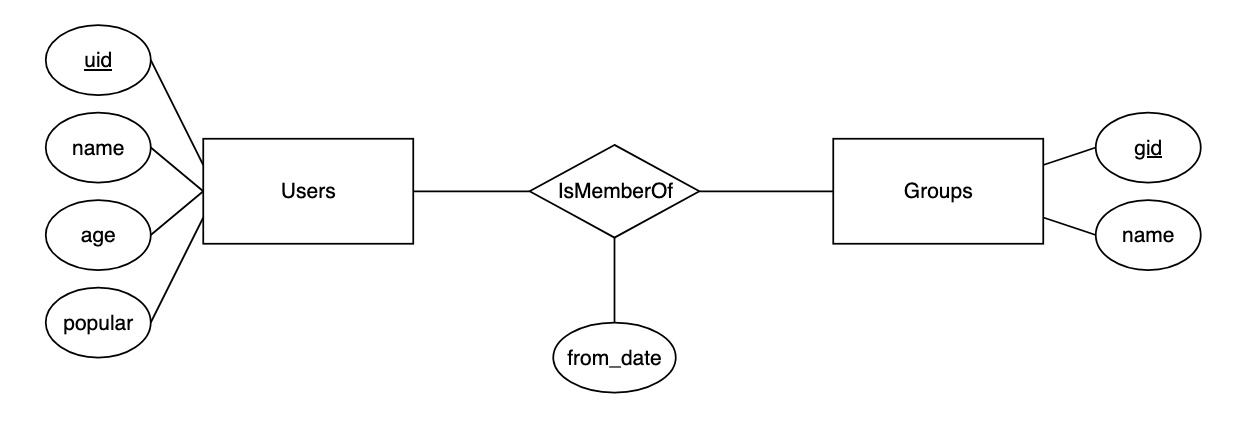
\includegraphics[scale=0.2]{img/social_media.png}
        \caption{Social media database ER diagram.} 
        \label{fig:social_media}
      \end{figure}

      Note that the \textit{from} attribute must be a part of the Member relation since it isn't uniquely associated with a user (a user can join multiple groups on different dates) or a group (two users can join a group on different dates). 
    \end{example}

    Therefore, we can associate an entity set and a relationship as relations. A minor detail is that relationships aren't really relations since the tuples in relations connect two entities, rather than the keys themselves, so some care must be taken to convert the entities into a set of attributes. 

    Therefore, we must determine if a relation models an entity or a relationship. There could also be multiple relationship sets between the same entity sets, e.g. if \textit{Member} and \textit{Likes} associates between \textit{Users} and \textit{Groups}. However, within a relationship set, there is an important set. 

    \begin{theorem}
      In a relationship set, each relationship is uniquely identified by the entities it connects. 
    \end{theorem}

    If there is an instance that someone joins, leaves, and rejoins a group, then we can modify our design by either: 
    \begin{enumerate}
      \item overwritting the first date joined 
      \item making another relation \textit{MembershipRecords} which has a date also part of the key, which will capture historical membership.  
    \end{enumerate}

    \subsubsection{Multiplicity of Binary Relationships}

      \begin{definition}[Multiplicity of Relationships]
        Given that $E$ and $F$ are entity sets, 
        \begin{enumerate}
          \item \textit{Many-many}: Each entity in E is related to $0$ or more entities in $F$ and vice versa. There are no restrictions, and we have \textit{IsMemberOf(\underline{uid}, \underline{gid})}. 

          \begin{figure}[H]
            \centering 
            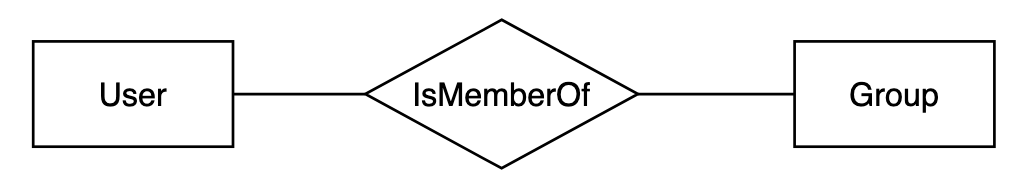
\includegraphics[scale=0.3]{img/ismember.png}
            \caption{} 
            \label{fig:ismember}
          \end{figure}


          \item \textit{Many-One}: Each entity in $E$ is related to $0$ or $1$ entity in $F$, but each entity in $F$ is related to $0$ or more in $E$. If $E$ points to $F$, then you can just think that this is an injective function, and we have \textit{IsOwnedBy(\underline{gid}, uid)}. If we have a rounded arrow, this means that for each group, its owner \textit{must} exist in \textit{Users} (so no $0$). 

          \begin{figure}[H]
            \centering 
            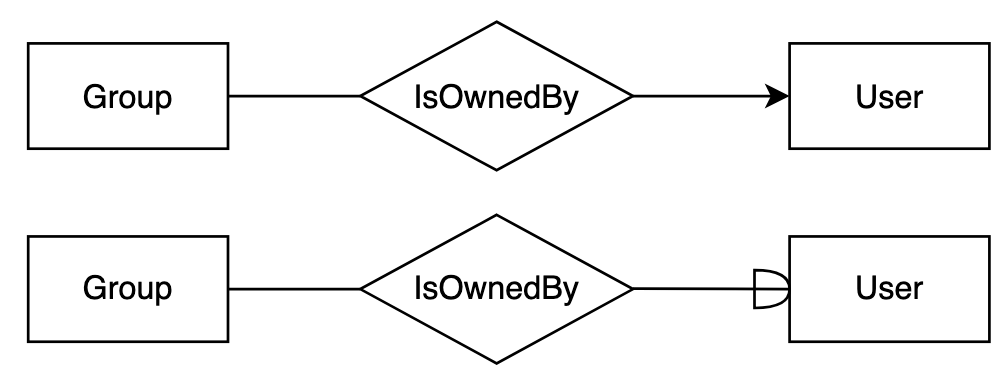
\includegraphics[scale=0.3]{img/isowned.png}
            \caption{} 
            \label{fig:isowned}
          \end{figure}


        \item \textit{One-One}: Each entity in $E$ is related to $0$ or $1$ entity in $F$ and vice versa. We can have either \textit{IsLinkedTo(\underline{uid}, twitter\_uid)} or \textit{IsLinkedTo(uid, \textit{twitter\_uid})} and must choose a primary key from these two possible keys.  

        \begin{figure}[H]
          \centering 
          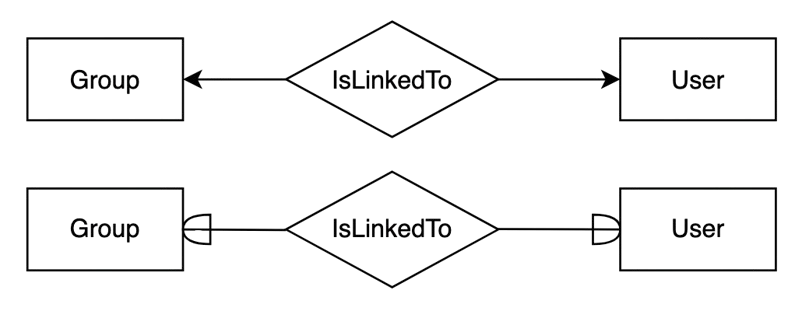
\includegraphics[scale=0.3]{img/islinked.png}
          \caption{} 
          \label{fig:islinked}
        \end{figure}

        \end{enumerate}
      \end{definition}


      You may notice that multiplicity and functional dependence are very similar that is. If we have two relations $R, S$ and have a relationship pointing from $R$ to $S$, then this states the FD $\mathbf{r} \mapsto \mathbf{s}$! Say that the keys are $\mathbf{k}_R, \mathbf{k}_S$, respectively. Then, we have 
      \begin{equation}
        \mathbf{k}_R \mapsto \mathbf{r} \mapsto \mathbf{s} \mapsto \mathbf{k}_S
      \end{equation} 

      \begin{example}[Movie Stars]
        Given the relations 
        \begin{enumerate}
          \item \textit{Movies(\underline{title, year}, length, name)}
          \item \textit{Stars(\underline{name}, address)} of a movie star and their address. 
          \item \textit{Studios(\underline{name}, address)} 
          \item \textit{StarsIn(\underline{star\_name}, \underline{movie\_name}, \underline{movie\_year})} 
          \item \textit{Owns(studio\_name, \underline{movie\_name}, \underline{movie\_year})}
        \end{enumerate}
        We have the following ER diagram 
        \begin{figure}[H]
          \centering 
          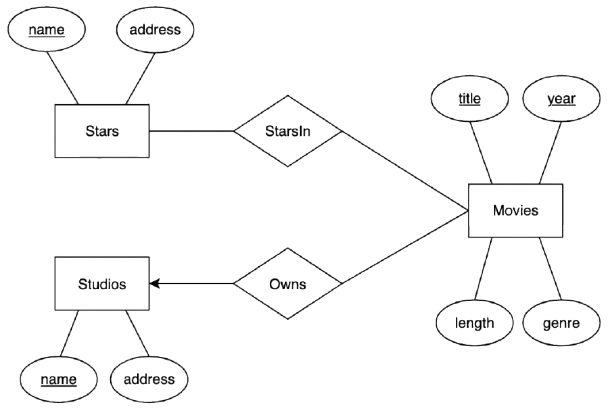
\includegraphics[scale=0.3]{img/movie_stars.png}
          \caption{Movie stars. } 
          \label{fig:movie_stars}
        \end{figure}
      \end{example}

      \begin{example}[Relationship within Itself]
        Sometimes, there is a relationship of an entity set with itself. This gives the relations 
        \begin{enumerate}
          \item \textit{Users(\underline{uid}, ...)} 
          \item \textit{IsFriendOf(\underline{uid1}, \underline{uid2})} 
          \item \textit{IsChildOf(\underline{child\_uid}, parent\_uid)}
        \end{enumerate}
        This can be modeled by the following. Note that 
        \begin{enumerate}
          \item users have no limitations on who is their friend. 
          \item assuming that all parents are single, a person can have at most one parent, so we have an arrow.  
        \end{enumerate}
        \begin{figure}[H]
          \centering 
          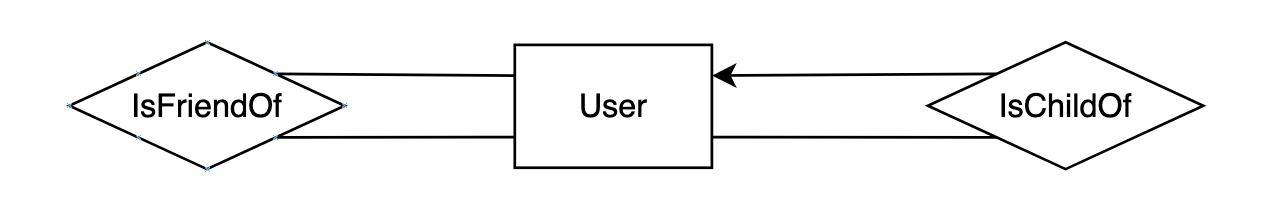
\includegraphics[scale=0.3]{img/within_itself.png}
          \caption{} 
          \label{fig:within_itself}
        \end{figure}
      \end{example}

    \subsubsection{Multiplicity of Multiway Relationships}

      Sometimes, it is necessary to have a relationship between 3 or more entity sets. It can be confusing to contruct the relations with the necessary keys. A general rule of thumb for constructing the relation of a relationship is 
      \begin{enumerate}
        \item Everything that the arrows point into are not keys.   
        \item Everything else are keys. So the arrow stumps are keys. 
      \end{enumerate}

      \begin{example}[Movie Stars]
        Suppose that we wanted to model \textit{Contract} relationship involving a studio, a star, and a movie. This relationships represents that a studio had contracted with a particular star to act in a particular movie. We want a contract to be owned by one studio, but one studio can have multiple contracts for different combinations of stars and movies. This gives the relations 
        \begin{enumerate}
          \item \textit{Stars(\underline{name}, address)} 
          \item \textit{Movies(\underline{title, year}, length, name)} 
          \item \textit{Studios(\underline{name}, address)} 
          \item \textit{Contracts(\underline{star\_name}, \underline{movie\_name}, studio\_name)}
        \end{enumerate}
        \begin{figure}[H]
          \centering 
          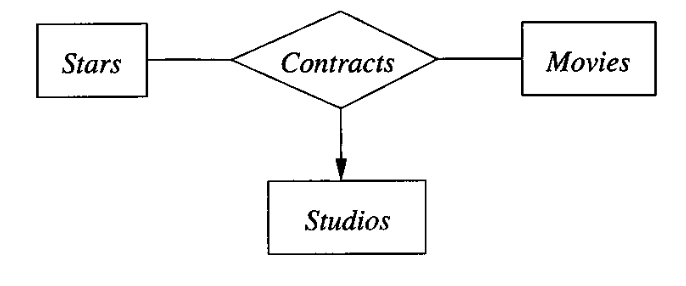
\includegraphics[scale=0.4]{img/contracts.png}
          \caption{} 
          \label{fig:contracts}
        \end{figure}
        We can make this even more complex by modifying contracts to have a studio of the star and the producing studio. 
        \begin{enumerate}
          \item \textit{Contracts(\underline{star\_name}, \underline{movie\_name}, produce\_studio\_name, star\_studio\_name)}
        \end{enumerate}
        \begin{figure}[H]
          \centering 
          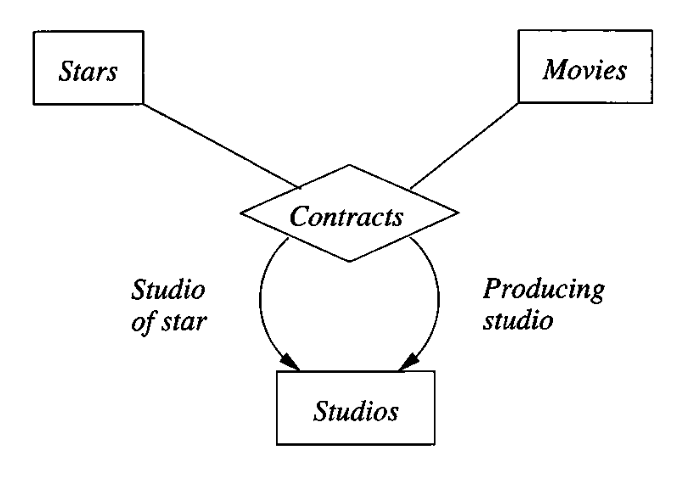
\includegraphics[scale=0.4]{img/four_ary.png}
          \caption{} 
          \label{fig:four_ary}
        \end{figure}
        Note that contracts can also have attributes, e.g. salary or time period. 
      \end{example}

      \begin{example}[Social Media]
        In a 3-ary relationship a user must have an initiator in order to join a group. In here, the \textit{isMemberOf} relation has an initiator, which must be unique for each initiated member, for a given group. 
        \begin{enumerate}
          \item \textit{User(\underline{uid}, ...)} 
          \item \textit{Group(\underline{gid}, ...)} 
          \item \textit{IsMemberOf(\underline{member}, initiator, \underline{gid})} since a member must have a unique pair of initiator/group that they are in. 
        \end{enumerate}
        \begin{figure}[H]
          \centering 
          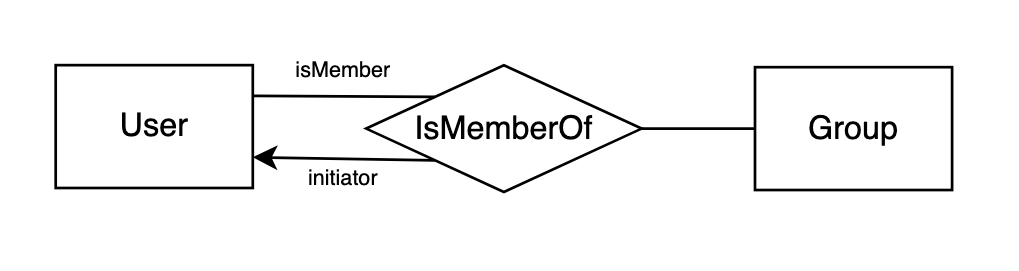
\includegraphics[scale=0.3]{img/three_ary.png}
          \caption{} 
          \label{fig:three_ary}
        \end{figure}
      \end{example}

      But can we model n-ary relationships with only binary relationships? Our intuition says we can't, for the same reasons that we get lossy decomposition into 2-attribute schemas when we try to satisfy BCNF. 
      \begin{figure}[H]
        \centering 
        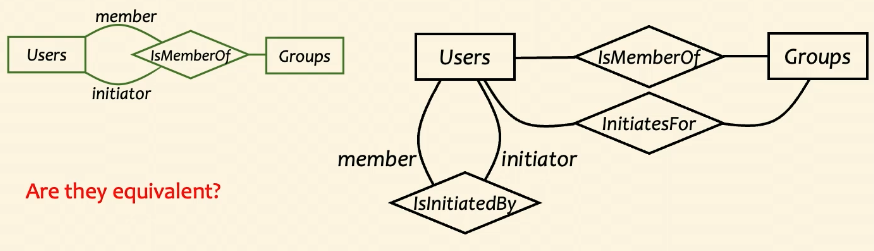
\includegraphics[scale=0.4]{img/nary_vs_binary.png}
        \caption{Attempt at reducing nary to binary ER relationships. } 
        \label{fig:}
      \end{figure}
      \begin{enumerate}
        \item u1 is in both g1 and g2, so \textit{IsMemberOf} contains both (u1, g1) and (u2, g2)
        \item u2 served as both an initiator in both g1 and g2, so \textit{InitiatesFor} contains both (g1, u2) and (g2, u2). 
        \item But in reality, u1 was initiated by u2 for g1 but not u2 for g2. This contradicts the information that you would get when joining the \textit{IsMemberOf} and \textit{InitiatesFor} relations. 
      \end{enumerate}
      Therefore, combining binary relations may generate something spurious that isn't included in the n-ary relationship. 

    \subsubsection{Subclasses of Entity Sets}

      Sometimes, an entity set contains certain entities that have special properties not associated with all members of the set. We model this by using a \textbf{isa} relationship with a triangle. 
      
      \begin{figure}[H]
        \centering 
        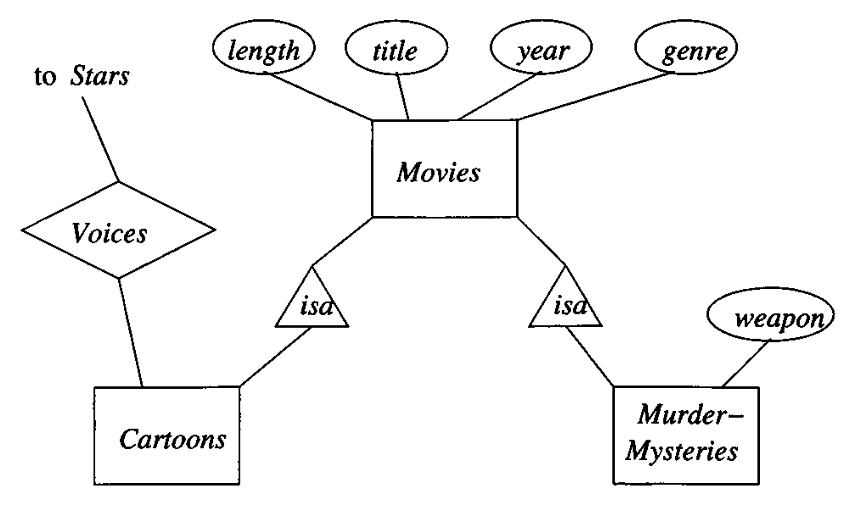
\includegraphics[scale=0.4]{img/isa.png}
        \caption{There are two types of movies: cartoons and murder-mysteries, which can have their own sub-attributes and their own relationships.} 
        \label{fig:isa}
      \end{figure}

      Suppose we have a tree of entity sets, connected by \textit{isa} relationships. A single entity consists of \textit{components} from one or more of these entity sets, and each component is inherited from its parent. 

  \subsection{Design Principles} 

    The first thing we should consider is the multiplicity, which is really context dependent. The second thing is redundancy, which we have mentioned through anomalies before.  

  \subsection{Weak Entity Sets}

    It is possible for an entity set's key to be composed of attributes, some or all of which belong to another entity set. There are two reasons why we need weak entity sets. 
    \begin{enumerate}
      \item Sometimes, entity sets fall into a hierarchy based on classifications unrelated to the \textit{isa} hierarchy. If entities of set $R$ are subunits of entities in set $F$, it is possible that the names of $R$-entities are not unique until we take into account the name of its $S$-entity.\footnote{Think of university rooms in different buildings.}
      \item The second reason is that we want to eliminate multiway relationships, which are not common in practice anyways. These weak entity sets have no attributes and have keys purely from its supporting sets. 
    \end{enumerate}

    \begin{definition}[Weak Entity Set]
      A \textbf{weak entity set} $R$ (double rectangles) depends on other sets. It is an entity set that 
      \begin{enumerate}
        \item has a key consisting of 0 or more of its own attributes, and 
        \item has key attributes from \textbf{supporting entity sets} that are reached by many-one \textbf{supporting relationships} (double diamonds) from it to other sets $S$. 
      \end{enumerate}
      It must satisfy the following. 
      \begin{enumerate}
        \item The relationship $T$ must be binary and many-one from $R$ to $S$. 
        \item $T$ must have referential integrity from $R$ to $S$ (since these are keys and therefore must exist in supporting sets), which is why we have a rounded arrow. 
        \item The attributes that $S$ supplies for the key of $R$ must be key attributes of $S$, unless $S$ is also weak, and it will get keys from its supporting entity set. 
        \item If there are several different supporting relationships from $R$ to the same $S$, then each relationship is used to supply a copy of the key attributes of $S$ to help form the key of $R$. 
      \end{enumerate}
      If an entity set supplies any attributes for its own key, then those attributes will be underlined. 
    \end{definition}

    \begin{example}
      To specify a location, it is not enough to specify just the seat number. The room number, and the building name must be also specified to provide the exact location. There are no extra attributes needed for this subclass, which is why a \textit{isa} relationship doesn't fit into this. 
      \begin{figure}[H]
        \centering 
        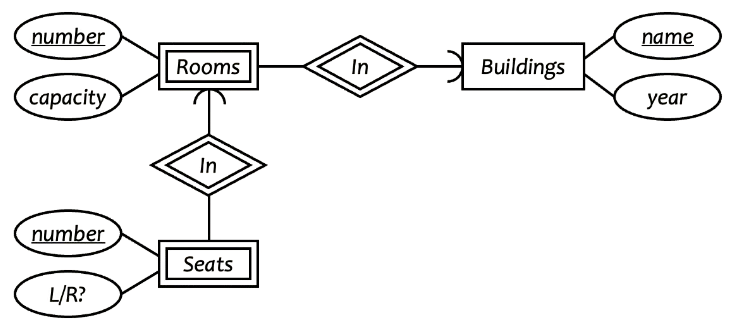
\includegraphics[scale=0.4]{img/weak_entity.png}
        \caption{Specifying a seat is not enough to determine the exact location in a university. We must know the room number and the building to fully identify it. Note that we must keep linking until we get to a regular, non-weak entity. } 
        \label{fig:weak_entity}
      \end{figure}
    \end{example}

    We generally want to use a weak entity set if an entity does not have attributes to define itself. 
    
    \begin{example}
      Say that we want to make a database with the constraints. 
      \begin{enumerate}
        \item For states, record the name and capital city. 
        \item For counties, record the name, area, and location (state) 
        \item For cities, record the name, population, and location (county and state) 
        \item Names of states should be unique. 
        \item Names of counties are unique within a state. 
        \item Names of cities are unique within a county. 
        \item A city is always located in a single county. 
        \item A county is always located in a single state. 
      \end{enumerate}
      Then, our ER diagram may look like 
      \begin{figure}[H]
        \centering 
        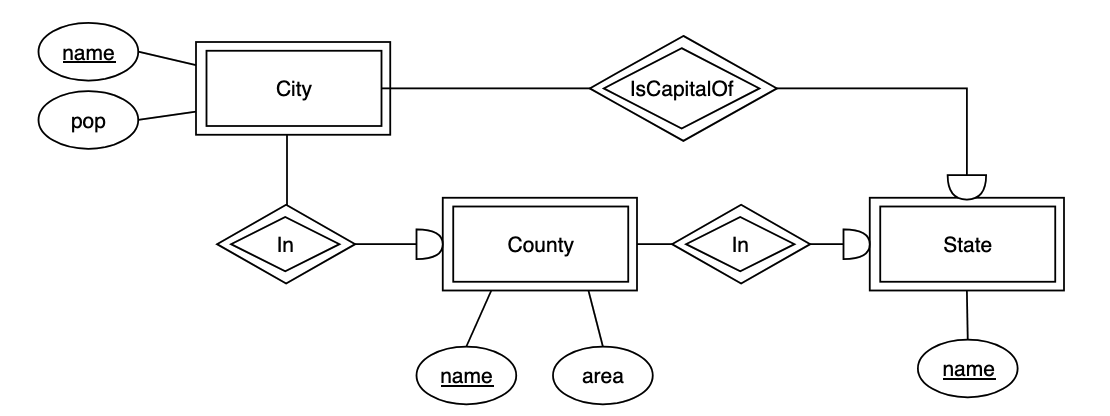
\includegraphics[scale=0.3]{img/city1.png}
        \caption{A weakness is that this doesn't prevent a city in state $X$ from being the capital of another state $Y$.} 
        \label{fig:city1}
      \end{figure}
    \end{example}

    \begin{example}
      Design a database with the following. 
      \begin{enumerate}
        \item A station has a unique name and address, and is either an express station or a local station. 
        \item A train has a unique number and engineer, and is either an express or local train. 
        \item A local train can stop at any station. 
        \item An express train only stops at express stations. 
        \item A train can stop at a station for any number of times during a train. 
        \item Train schedules are the same every day. 
      \end{enumerate}
      Then, our ER diagram may look like 
      \begin{figure}[H]
        \centering 
        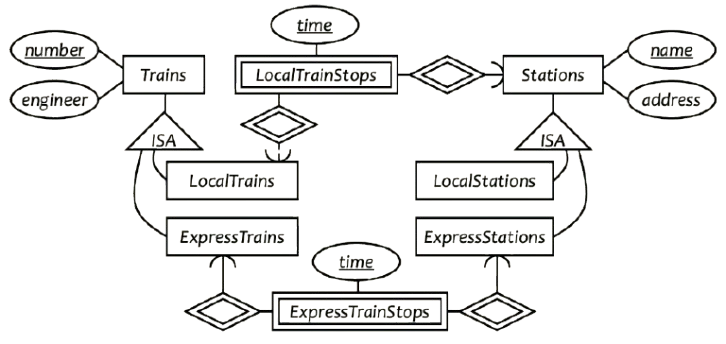
\includegraphics[scale=0.4]{img/train1.png}
        \caption{} 
        \label{fig:train1}
      \end{figure}
      
    \end{example}

  \subsection{Translating ER Diagrams to Relational Designs}

    One a simple level, converting an ER diagram to a relational database schema is straightforward. Here are some rules we list. 

    \begin{theorem}[Converting Entity Sets]
      Turn each entity set into a relation with the same set of attributes. 
    \end{theorem}

    \begin{theorem}[Converting Relationships]
      Replace a relationship by a relation whose attributes are the keys for the connected entity sets along with its own attributes. If an entity set is involved several times in a relationship, then its key attributes are repeated, so you must rename them to avoid duplication.
    \end{theorem}

    \begin{theorem}[Reduce Repetition for Many-One Relationships]
      We can actually reduce repetition for many-one relationships. For example, if there is a many-one relationship $T$ from relation $R$ to relation $S$, then $\mathbf{r}$ functionally determines $\mathbf{s}$, so we can combine them into one relation consisting of 
      \begin{enumerate}
        \item all attributes of $R$. 
        \item key attributes of $S$. 
        \item Any attributes belonging to relationship $T$. 
      \end{enumerate}
    \end{theorem}
    
    \begin{theorem}[Handling Weak Entity Sets]
      To build weak entity sets, we must do three things. 
      \begin{enumerate}
        \item The relation for weak entity set $W$ must include its own attributes, all key (but not non-key) attributes of supporting entity sets, and all attributes for supporting relationships for $W$. 
        \item The relation for any relationship where $W$ appears must use the entire set of keys gotten from $W$ and its supporting entity sets. 
        \item Supporting relationships should not be converted since they are many-one, so we can use the reduce repetition for many-one relationships rule above. 
      \end{enumerate}
    \end{theorem}

    \begin{example}
      To translate the seat, rooms, and buildings diagram, 
      \begin{figure}[H]
        \centering 
        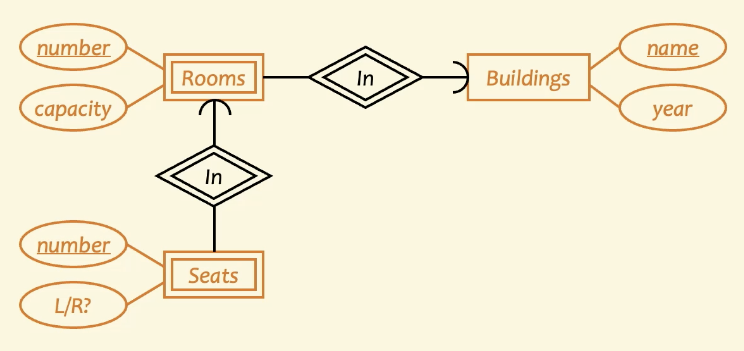
\includegraphics[scale=0.4]{img/seat.png}
        \caption{} 
        \label{fig:seat}
      \end{figure}
      we have 
      \begin{enumerate}
        \item \textit{Building(\underline{name}, year)} 
        \item \textit{Room(\underline{building\_name}, \underline{room\_num}, capacity)}
        \item \textit{Seat(\underline{building\_name}, \underline{room\_num}, \underline{seat\_num}, left\_or\_right)}
      \end{enumerate}
      Note that we do not need to convert the relationships since they are contained within the entity set relations. So ignore double diamonds. 
    \end{example}

    \begin{figure}[H]
      \centering 
      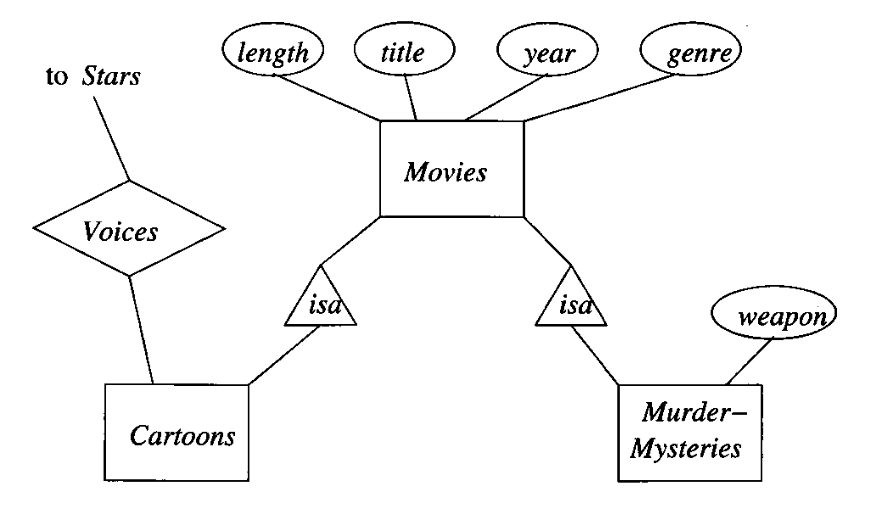
\includegraphics[scale=0.3]{img/movie_hierarchy.png}
      \caption{A figure of the movie hierarchy for convenience. } 
      \label{fig:movie_hierarchy}
    \end{figure}

    \begin{theorem}[Converting Subclass Structures]
      To convert subclass structure with a \textit{isa} hierarchy, there are multiple ways we can convert them. 
      \begin{enumerate}
        \item \textit{E/R Standard}. An entity is in all superclasses and only contains the attributes its own subclass. For each entity set $R$ in the hierarchy, create a relation that includes the key attributes from the root and any attributes belonging to $R$. This gives us 
          \begin{enumerate}
            \item \textit{Movies(title, year, length, genre)}
            \item \textit{MurderMysteries(title, year, weapon)}
            \item \textit{Cartoons(title, year)}
          \end{enumerate}
        \item \textit{Object Oriented}. For each possible subtree that includes the root, create one relation whose schema includes all the attributes of all entity sets in the subtree.
          \begin{enumerate}
            \item \textit{Movies(title, year, length, genre)} 
            \item \textit{MoviesC(title, year, length, genre)} 
            \item \textit{MoviesMM(title, year, length, genre, weapon)}
            \item \textit{MoviesCMM(title, year, length, genre, weapon)}
          \end{enumerate}
          Additionally, the relationship would be \textit{Voices(title, year, starName)}. 
        \item \textit{Null Values}. Create one relation for the entire hierarchy containing all attributes of all entity sets. Each entity is one tuple, and the tuple has null values for attributes the entity does not have. We would in here always have a single schema. 
          \begin{enumerate}
            \item \textit{Movie(title, year, length, genre, weapon)}
          \end{enumerate}
      \end{enumerate}
    \end{theorem}

    Note that the difference between the first two is that in ER, \textit{MurderMysteries} does not contain the attributes of its superclass, while in OO, it does. 

    As you probably notice, each standard has pros and cons. The nulls approach uses only one relation, which is simple and nice. To filter out over all movies, E/R is nice since we only filter through \textit{Movies}, whilst in OO we have to go through all relations. However, when we want to filter movies that are both Cartoons and Murder Mysteries, then OO is better since we can only select from \textit{MoviesCMM} rather than having to go through multiple relations for ER or filter out with further selections in Null. Also, OO uses the least memory, since it doesn't waste space on null values on attributes.  


    \begin{example}
      Let's put this all together to revisit the train station example. 
      \begin{figure}[H]
        \centering 
        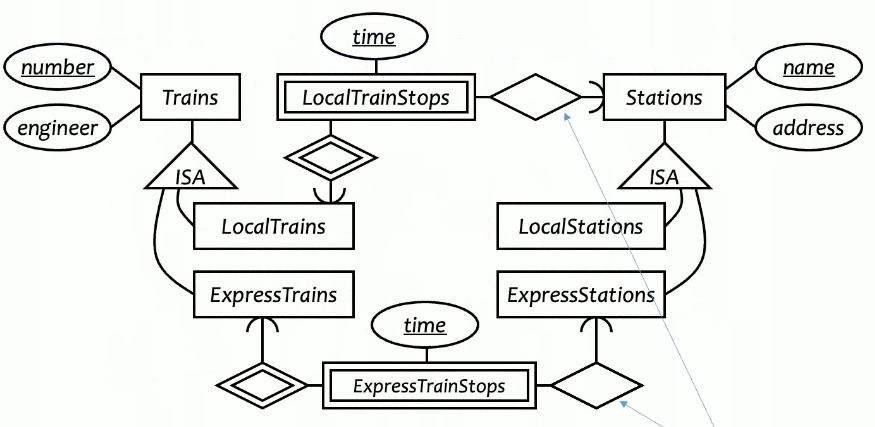
\includegraphics[scale=0.4]{img/final_station.png}
        \caption{For convenience} 
        \label{fig:final_station}
      \end{figure}
      We can use the ER standard to define the first 6 regular relations in single rectangles.  
      \begin{enumerate}
        \item \textit{Train(\underline{number}, engineer)}
        \item \textit{LocalTrain(\underline{number}}
        \item \textit{ExpressTrain(\underline{number}}
        \item \textit{Station(\underline{name}, address)}
        \item \textit{LocalStation(\underline{name})}
        \item \textit{ExpressStation(\underline{name})}
      \end{enumerate}
      Then we can construct the weak entity sets. 
      \begin{enumerate}
        \item \textit{LocalTrainStops(\underline{local\_train\_num}, \underline{time})}
        \item \textit{ExpressTrainStops(\underline{express\_train\_num}, \underline{time})}
      \end{enumerate}
      Then we can construct the relationships (marked with the arrows).  
      \begin{enumerate}
        \item \textit{LocalTrainStopsAtStation(\underline{local\_train\_number}, \underline{time}, station\_name)}
        \item \textit{ExpressTrainStopsAtStation(\underline{express\_train\_number}, \underline{time}, express\_station\_name)}
      \end{enumerate}
      Note that we can simplify these 10 relations to 8. For example, the \textit{LocalTrain} and \textit{LocalStation} relations are redundant since it can be computed as 
      \begin{align}
        LocalTrain & = \pi_{number} (Train) - ExpressTrain \\
        LocalStation & = \pi_{number} (Station) - ExpressStation
      \end{align}
      There is a tradeoff since it's an extra computation when checking. However, if we had used the Null Value strategy, this would be a lot simpler, and we can use value constraints on the train and station type, which can be implemented in the DBMS (though not directly in the ER diagram). 
    \end{example}

\section{Intermediate SQL} 

    We have went over the basic SQL queries that were directly translations of relational algebra. 

  \subsection{Bags}

    We were used to working with sets, which don't allow duplicate elements, but let's talk about \textit{multisets}, or \textbf{bags}, which do. Why is this advantageous? 
    \begin{enumerate}
      \item To take the union of two bags, we can just add everything into the other without going through to check for duplicates. 
      \item When we project relations as bags, we also don't need to search through all pairs to find duplicates. 
    \end{enumerate}
    This allows for efficiency at the cost of memory. 

    Recall that the \texttt{UNION}, \texttt{EXCEPT}, and \texttt{INTERSECT} are set semantics that removes duplicates in the input tables first and then removes duplicates in the result. 

    \begin{definition}[Bag Operations]
      However, we can also use bag semantics. We can think of each row $a$ having an implicit count of times $c_a$ it appears in the table.  
      \begin{enumerate}
        \item \textbf{Bag union} sums up the counts from two tables. 
        \item \textbf{Bag difference} does a proper-subtract\footnote{Subtracts the counts and truncates counts to $0$ if negative. So $\{a, a\} - \{a, a, a\} = \{\}$.} 
        \item \textbf{Bag intersection} takes the minimum of the two counts. 
      \end{enumerate}
      This is analogous to the \texttt{UNION ALL}, \texttt{EXCEPT ALL}, and \texttt{INTERSECT ALL} operations in SQL. Given that 
      \begin{enumerate}
        \item $\mathrm{Bag1} = \{1, 1, 2\}$
        \item $\mathrm{Bag2} = \{1, 2, 2\}$
      \end{enumerate}
      We have 
      \begin{lstlisting}
        (SELECT * FROM Bag1) 
        UNION ALL 
        (SELECT * FROM Bag2);     // {1, 1, 1, 2, 2, 2}

        (SELECT * FROM Bag1) 
        EXCEPT ALL 
        (SELECT * FROM Bag2);     // {1}

        (SELECT * FROM Bag1) 
        INTERSECT ALL 
        (SELECT * FROM Bag2);     // {1, 2}
      \end{lstlisting}
    \end{definition}

    \begin{example}
      Look at these two operations on the schema \texttt{Poke(uid1, uid2, timestamp)}. 

      \noindent\begin{minipage}{.5\textwidth}
      \begin{lstlisting}[]{Code}
        (SELECT uid1 FROM Poke) 
        EXCEPT 
        (SELECT uid2 FROM Poke); 
      \end{lstlisting}
      \end{minipage}
      \hfill
      \begin{minipage}{.49\textwidth}
      \begin{lstlisting}[]{Output}
        (SELECT uid1 FROM Poke) 
        EXCEPT ALL
        (SELECT uid2 FROM Poke); 
      \end{lstlisting}
      \end{minipage}
      The first operation returns all users who poked others but were never poked, while the second returns all users who poked others more than they were poked. 
    \end{example}

  \subsection{Nested Queries and Subqueries} 

    We have so far worked with a single query consisiting of a single select statement. However, we can extend this. 

    \begin{definition}[\texttt{EXISTS}]
      The \texttt{EXISTS}(subquery) keyword checks if a subquery is empty or not, and \texttt{NOT EXISTS} checks the negation. 
    \end{definition}

    \begin{example}[Ages]
      Given \textit{User(name, age)}, say that we want to get all users whose age is equal to a person named Bart. Then, we want to select all users from the relation. For each user, we perform the subquery where this original tuple age coincides the others age and the others name is Bart. The outer query only returns those rows for which the \texttt{EXISTS} subquery returned true. Then we can write the two equivalent queries. 

      \noindent\begin{minipage}{.5\textwidth}
      \begin{lstlisting}[]{Code}
        SELECT * 
        FROM User as u
        WHERE EXISTS(SELECT * FROM User
                      WHERE name = "Bart" 
                      AND age = u.age); 
      \end{lstlisting}
      \end{minipage}
      \hfill
      \begin{minipage}{.49\textwidth}
      \begin{lstlisting}[]{Output}
        SELECT * 
        FROM User 
        WHERE age IN(SELECT age 
                      FROM User 
                      WHERE name = 'Bart'); 
      \end{lstlisting}
      \end{minipage}

      The left is a \textbf{correlated subquery}, which is a query that needs a parameter from the main query and are generally slower. To understand this, you should always look in the following order. 
      \begin{enumerate}
        \item \texttt{FROM}. Look at where we are querying from. 
        \item \texttt{WHERE}. Find out if this condition is satisfied. 
        \item \texttt{SELECT}. Return all tuples that satisfies this condition. 
      \end{enumerate}
      However, this is not actually how the database system will do this. It will do it in an equivalent but more efficient way. 
    \end{example}

    Here is a very useful keyword that simplifies complex nested queries, one example of a \textbf{common table expression (CTEs)}. 
    
    \begin{definition}[\texttt{WITH}]
      The \texttt{WITH} clause aliases many relations returned from queries. 
      \begin{lstlisting}
        WITH Temp1 AS (SELECT ...), 
             Temp2 AS (SELECT ...) 
        SELECT X, Y 
        FROM Temp1, Temp2 
        WHERE ...
      \end{lstlisting}
    \end{definition}

    \begin{example}
      To extend the Bart age example, we can think of temporarily storing a query of only Bart's ages, and then comparing it when doing the main query over \textit{User}. 
      \begin{lstlisting}
        WITH BartAge AS 
          (SELECT age 
          FROM User 
          WHERE name = 'Bart') 
        SELECT U.uid, U.name, U.pop, 
        FROM User U, BartAge B 
        WHERE U.age = B.age; 
      \end{lstlisting}
    \end{example}

  \subsection{Aggregate Functions} 

    \begin{definition}[Standard SQL Aggregate Functions]
      The aggregate functions offered are 
      \begin{enumerate}
        \item \texttt{COUNT} counts the number of rows in a query. \texttt{COUNT(DISTINCT att)} counts the distinct count of an attribute in a query. 
        \item \texttt{SUM} counts the sum of the values of an attribute in a query. 
        \item \texttt{AVG} is the average. 
        \item \texttt{MIN} is the minimum of an attribute. 
        \item \texttt{MAX} is the maximum of an attribute. 
      \end{enumerate}
    \end{definition}

    \begin{example}
      If we want to find the number of users under 18 and their average popularity, then we can write 
      \begin{lstlisting}
        SELECT COUNT(*), AVG(pop) 
        FROM User 
        WHERE age < 18; 
      \end{lstlisting}
    \end{example}

  \subsection{Group By} 

    \begin{definition}[\texttt{GROUP BY}]
      \texttt{GROUP BY att} is used when you want to group the query by equal values of the attributes. The syntax is 
      \begin{lstlisting}
        SELECT ... FROM ... WHERE ... 
        GROUP BY age; 
      \end{lstlisting}
      To parse this, first form the groups based on the same values of all attributes in the group by clause. Then, output only one row in the select clause per group. We can look at the following order
      \begin{enumerate}
        \item \texttt{FROM}. Look at where we are querying from. 
        \item \texttt{WHERE}. Find out if this condition is satisfied to filter the main query. 
        \item \texttt{GROUP BY}. Group rows according to the values of the GROUP BY columns. 
        \item \texttt{SELECT}. Compute the select query for each group. The number of groups should be equal to the number of rows in the final output. 
      \end{enumerate}
      Note that if a query uses aggregation/group by, every column referenced in select must be either aggregated or a group by column. 
    \end{definition}

    \begin{example}
      If we want to find the number of users in a certain age and their average popularity, for all ages, then we can write 
      \begin{lstlisting}
        SELECT age, AVG(pop) 
        FROM Usere
        GROUP BY age; 
      \end{lstlisting}
      You don't necessarily have to report the group by attribute in the select. The two following examples are perfectly fine, though in the right query, \texttt{age} may not functionally determine \texttt{AVG(pop)}. 

      \noindent\begin{minipage}{.5\textwidth}
      \begin{lstlisting}[]{Code}
        SELECT AVG(pop) 
        FROM User
        GROUP BY age; 
        
      \end{lstlisting}
      \end{minipage}
      \hfill
      \begin{minipage}{.49\textwidth}
      \begin{lstlisting}[]{Output}
        SELECT age, AVG(pop)  
        FROM User 
        GROUP BY age, name; 
      \end{lstlisting}
      \end{minipage}

      However, this left query is not syntactically correct since \texttt{name} is not in the group by clause or aggregated. This is true even if \texttt{age} functionally determines \texttt{name}. Neither is the right since the lack of a group by clause means that the aggregate query is over the entire relation, which has multiple uid values. 

      \noindent\begin{minipage}{.5\textwidth}
      \begin{lstlisting}[]{Code}
        SELECT age, name, AVG(pop) 
        FROM User
        GROUP BY age; 
      \end{lstlisting}
      \end{minipage}
      \hfill
      \begin{minipage}{.49\textwidth}
      \begin{lstlisting}[]{Output}
        SELECT uid, MAX(pop) 
        FROM User; 
        .
      \end{lstlisting}
      \end{minipage}
    \end{example}

    As you can see, this is great to use for aggregate functions. If there is no group by clause, this is equivalent to grouping everything together.  

    \begin{example}
      Given the relation 

      \begin{table}[H]
        \centering
        \begin{tabular}{|c|c|c|}
          \hline
          \textbf{A} & \textbf{B} & \textbf{C} \\
          \hline
          1 & 1 & 10 \\ 
          2 & 1 & 8 \\ 
          1 & 1 & 10 \\ 
          2 & 3 & 8 \\ 
          2 & 1 & 6 \\ 
          2 & 2 & 2 \\ 
          \hline
        \end{tabular}
        \caption{Original relation. }
        \label{tab:groupby}
      \end{table}
    
      Running the query 
      \begin{lstlisting}
        SELECT A, B, SUM(C) AS S 
        FROM R 
        GROUP BY A, B; 
      \end{lstlisting}
      gives 
      
      \begin{table}[H]
        \centering
        \begin{tabular}{|c|c|c|}
          \hline
          \textbf{A} & \textbf{B} & \textbf{S} \\
          \hline
          1 & 1 & 20 \\ 
          2 & 1 & 14 \\ 
          2 & 3 & 8 \\ 
          2 & 2 & 2 \\ 
          \hline
        \end{tabular}
        \caption{Our query. }
        \label{tab:groupby_output}
      \end{table}
    \end{example}

  \subsection{Having} 

    \begin{definition}[\texttt{HAVING}]
      If you want to filter out groups having certain conditions, you must use the \texttt{HAVING} keyword rather than \texttt{WHERE}. The syntax is 
      \begin{lstlisting}
        SELECT A, B, SUM(C) FROM ... WHERE ... 
        GROUP BY ... 
        HAVING SUM(C) < 10; 
      \end{lstlisting}
      You should look at the \texttt{HAVING} clause after you look at the \texttt{GROUP BY} but before \texttt{SELECT}. 
    \end{definition}

    \begin{example}
      Given the relation 

      \begin{table}[H]
        \centering
        \begin{tabular}{|c|c|c|}
          \hline
          \textbf{A} & \textbf{B} & \textbf{C} \\
          \hline
          1 & 1 & 10 \\ 
          2 & 1 & 8 \\ 
          1 & 1 & 10 \\ 
          2 & 3 & 8 \\ 
          2 & 1 & 6 \\ 
          2 & 2 & 2 \\ 
          \hline
        \end{tabular}
        \caption{Original relation. }
        \label{tab:groupby2}
      \end{table}
    
      Running the query 
      \begin{lstlisting}
        SELECT A, B, SUM(C) AS S 
        FROM R 
        GROUP BY A, B 
        HAVING SUM(C) > 8; 
      \end{lstlisting}
      gives 
      
      \begin{table}[H]
        \centering
        \begin{tabular}{|c|c|c|}
          \hline
          \textbf{A} & \textbf{B} & \textbf{S} \\
          \hline
          1 & 1 & 20 \\ 
          2 & 1 & 14 \\ 
          \hline
        \end{tabular}
        \caption{Our query. }
        \label{tab:groupby2_output}
      \end{table}
    \end{example}

    \begin{example}
      Given the schema \texttt{Sailor(sid, name, age, rating)}, to find the age of the youngest sailor with age at least 18, for each rating with at least 2 sailors, we can run the query. 
      \begin{lstlisting}
        SELECT S.rating, MIN(S.age) AS minage 
        FROM Sailors S 
        WHERE S.age >= 18
        GROUPBY S.rating 
        HAVING COUNT(*) > 1; 
      \end{lstlisting}

      \begin{figure}[H]
        \centering 
        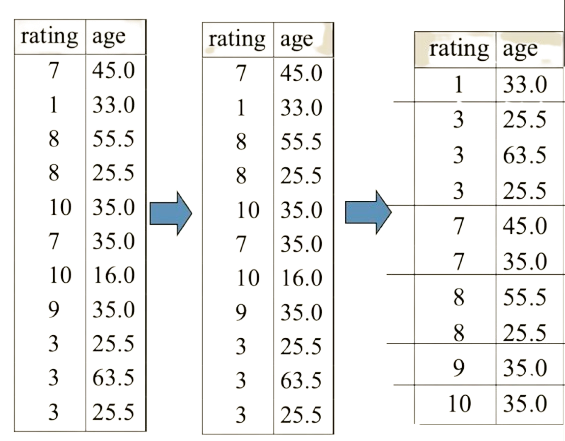
\includegraphics[scale=0.4]{img/sailors.png}
        \caption{The thought process.} 
        \label{fig:thought}
      \end{figure}
    \end{example}

    \begin{definition}[Scalar Subqueries]
      Sometimes, if a query returns 1 scalar, then you can use it in your \texttt{WHERE} clause. You must be sure that a query will return exactly 1 scalar (not $0$ and not more than $1$), or there will be a runtime error.  
    \end{definition}

    \begin{example}
      If we want to compute users with the same age as Bart, we can write 
      \begin{lstlisting}
        SELECT * FROM User 
        WHERE age = (SELECT age from User WHERE name = 'Bart'); 
      \end{lstlisting}
      However, we may not know if Bart functionally determines age, so we must be careful. 
    \end{example}

  \subsection{Quantified Subqueries}

    \begin{definition}[\texttt{ALL}, \texttt{ANY}]
      We have the following \textbf{quantified subqueries}, which performs a broadcasting condition and checks if all (\texttt{ALL}) or any (\texttt{ANY}) are true. 
    \end{definition}

    \begin{example}[Popular Users]
      Which users are the most popular? We can write this in two ways. 

      \noindent\begin{minipage}{.5\textwidth}
      \begin{lstlisting}[]{Code}
        SELECT * 
        FROM User 
        WHERE pop >= ALL(SELECT pop from User); 
        .
      \end{lstlisting}
      \end{minipage}
      \hfill
      \begin{minipage}{.49\textwidth}
      \begin{lstlisting}[]{Output}
        SELECT * 
        FROM User 
        WHERE NOT 
          (pop < ANY(SELECT pop from User)); 
      \end{lstlisting}
      \end{minipage}

      To review, here are more ways you can do the same query. 

      \noindent\begin{minipage}{.5\textwidth}
      \begin{lstlisting}[]{Code}
        SELECT * 
        FROM User AS u 
        WHERE NOT EXISTS  
          (SELECT * FROM User
          WHERE pop > u.pop); 
      \end{lstlisting}
      \end{minipage}
      \hfill
      \begin{minipage}{.49\textwidth}
      \begin{lstlisting}[]{Output}
        SELECT * FROM User 
        WHERE uid NOT IN 
          (SELECT u1.uid
          FROM User as u1, User as u2 
          WHERE u1.pop < u2.pop); 
      \end{lstlisting}
      \end{minipage}
    \end{example}

  \subsection{Incomplete Information}

    We are not guaranteed that we will have all data. What if there are some null values? We need some way to handle unknown or missing attribute values. 

    One way is to use a default value (like $-1$ for age), but this can mess with other operations, such as getting average values of certain groups of users, or can make computations harder since we have to first filter out users with \texttt{age=-1} before querying. 

    Another way is to use a valid bit for every attribute. For example, \textit{User(uid, name, age)} could map to \textit{User(uid, name, name\_valid, age, age\_valid)}, but this is not efficient as well. 

    A better solution is to decompose the table into multiple relations such that a missing value indicates a missing row in one of the subrelations. For example, we can decompose \texttt{User(uid, name, age, pop)} to 
    \begin{enumerate}
      \item \textit{UserID(uid)}
      \item \textit{UserName(uid, name)}
      \item \textit{UserAge(uid, age)}
      \item \textit{UserPop(uid, pop)}
    \end{enumerate}
    This is conceptually the cleanest solution but also complicates things. Firstly, the natural join wouldn't work, since compared to a single table with null values, the natural join of these tables would exclude all tuples that have at least one null value in them. 


    \begin{definition}[\texttt{NULL}]
      SQL's solution is to have a special value \texttt{NULL} indicating an unknown but not empty value. It has the following properties. 
      \begin{enumerate}
        \item It holds for every domain (null is the same for booleans, strings, ints, etc.). 
        \item Any operations like $+, -, \times, >$... leads to a \texttt{NULL} value. 
        \item All aggregate functions except \texttt{COUNT} return a \texttt{NULL}. \texttt{COUNT} also counts null values. 
      \end{enumerate}
    \end{definition}

    \begin{theorem}[Three-Valued Logic]
      Here is another way to implement the unknown logic with \textit{three-valued logic}. Suppose we set True=1, False=0. Then we can see that given statements $x, y$ which evaluate to $0, 1$, 
      \begin{enumerate}
        \item $x$ and $y$ is equivalent to $\min(x, y)$
        \item $x$ or $y$ is equivalent to $\max(x, y)$ 
        \item not $x$ is equivalent to $1 - x$
      \end{enumerate}
      It turns out that if we set unknown=0.5, then this logic also works out very nicely. Check it yourself. Therefore, \texttt{WHERE} and \texttt{HAVING} clauses only select rows for which the condition is True, not False or Unknown. 
    \end{theorem}

    \begin{example}[Warnings]
      Note that null breaks a lot of equivalences, leading to unintended consequences. 
      \begin{enumerate}
        \item The two are not equivalent since if we have nulls, the average ignores all nulls, while the second query will sum up all non-nulls and divide by the count including the nulls. 
        \begin{lstlisting}
          SELECT AVG(pop) FROM User; 
          SELECT SUM(pop) / COUNT(*) FROM User; 
        \end{lstlisting}

        \item The two are also not equivalent since \texttt{pop = pop} is not True, but Unknown, for nulls, so it would not return nulls. The first query would return all tuples, even nulls. 
        \begin{lstlisting}
          SELECT * from User; 
          SELECT * from User WHERE pop = pop; 
        \end{lstlisting}

        \item Never compare equality with null, since this never outputs True. Rather, you should use the special keywords \texttt{IS NULL} and \texttt{IS NOT NULL}. 
          \begin{lstlisting}
            SELECT * FROM User WHERE pop = NULL; // never returns anything 
            SELECT * FROM User WHERE pop IS NULL; // correct 
          \end{lstlisting}
      \end{enumerate}
    \end{example}


  \subsection{Joins} 
    
    Take a look at the following motivating example. Suppose we want to find all members and their respective groups from \textit{Group(gid, name)}, \textit{Member(uid, gid)}, \textit{User(uid, name)}. Then we can write the query 
    \begin{lstlisting}
      SELECT g.gid, g.name AS gname, 
          u.uid, u.name AS uname 
      FROM Group g, Member m, User u 
      WHERE g.gid = m.gid AND m.uid = u.uid; 
    \end{lstlisting}
    This looks fine, but what happens if \textit{Group} is empty? That is, there is a group in the \textit{Group} relation but does not appear in the \textit{Member} relation. Then, \texttt{m.gid} will evaluate to False and would not appear in the joined table, which is fine, but what if we wanted to make sure all groups appeared in this master membership table? If a group is empty, we may want it to just have null values for \texttt{uid} and \texttt{uname}. In this case, we want to use outer join. 

    \begin{definition}[Outer Joins]
      An outer join guarantees that we have all elements in one or more tables. 
      \begin{enumerate}
        \item \texttt{(INNER) JOIN}: Returns records that have matching values in both tables, with the notation $R \bowtie S$. 
        \item \texttt{LEFT (OUTER) JOIN}: Returns all records from the left table, and the matched records from the right table with potential NULLs, with notation $R \lojoin S$. 
        \item \texttt{RIGHT (OUTER) JOIN}: Returns all records from the right table, and the matched records from the left table with potential NULLs, with notation $R \rojoin S$. 
        \item \texttt{FULL (OUTER) JOIN}: Returns all records when there is a match in either left or right table with potential NULLs, with notation $R \fojoin S$. 
      \end{enumerate}

      \begin{figure}[H]
        \centering 
        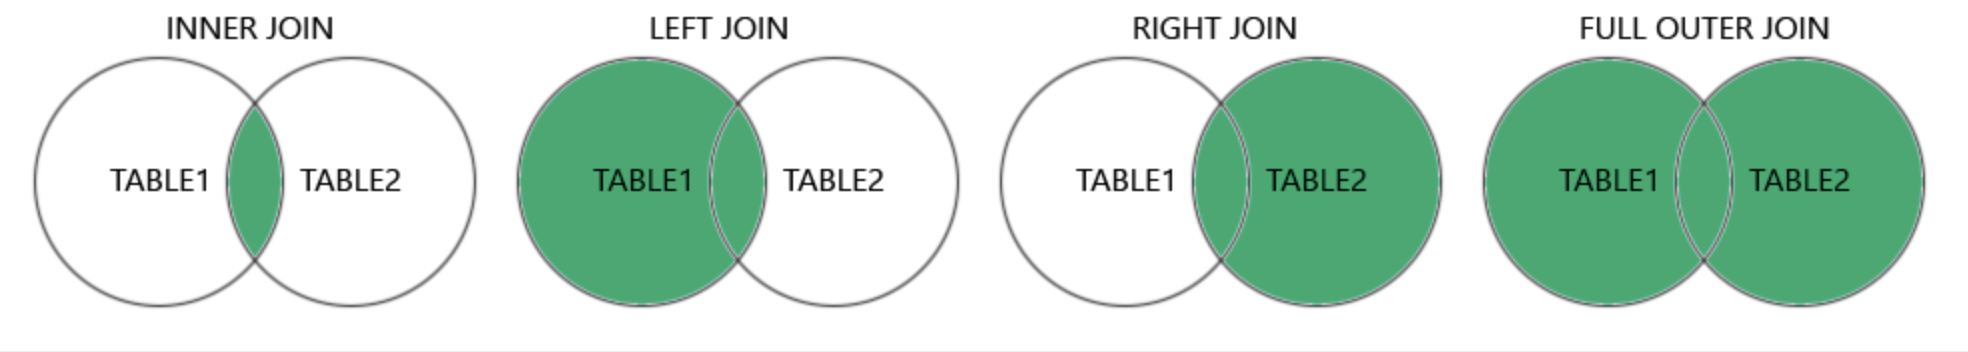
\includegraphics[scale=0.4]{img/outerjoin.png}
        \caption{Nice diagram from W3Schools.} 
        \label{fig:outerjoin}
      \end{figure}

      The SQL syntax is below. 
      \begin{lstlisting}
        // inner joins, you can use ON rather than WHERE
        SELECT * FROM Group JOIN Member
          ON Group.gid = Member.gid; 

        SELECT * FROM Group LEFT OUTER JOIN Member
          ON Group.gid = Member.gid; 

        SELECT * FROM Group RIGHT OUTER JOIN Member
          ON Group.gid = Member.gid; 

        SELECT * FROM Group RIGHT OUTER JOIN Member
          ON Group.gid = Member.gid; 
      \end{lstlisting}
    \end{definition}

    \begin{example}[Complex Example with Beers]
      Given the schemas 
      \begin{enumerate}
        \item \textit{Frequents(drinker, bar, times\_a\_week)}, 
        \item \textit{Serves(bar, beer, price)}, 
        \item \textit{Likes(drinker, beer)}, 
      \end{enumerate}
      say that we want to select drinkers and bars that visit the bars at least 2 times a week and the bars serves at least 2 beers liked by the drinker and count the number of beers served by the bars that are liked by the drinker. The query is shown below. 

      \begin{lstlisting}
        SELECT F.drinker, F.bar, COUNT(L.beer) 
        FROM Frequents F, Serves S, Likes L 
        WHERE F.drinker = L.drinker
          AND F.bar = S.bar 
          AND L.beer = S.beer 
          AND F.times_a_week >= 2 
        GROUP BY F.drinker, F.bar 
        HAVING COUNT(L.beer) >= 2 
      \end{lstlisting}
    \end{example}

  \subsection{Inserting, Deleting, and Updating Tuples}

    We have briefly saw how to create and drop tables. To update a table, we can do the following. 

    \begin{definition}[\texttt{INSERT}]
      You can either 
      \begin{enumerate}
        \item insert one row  
          \begin{lstlisting}
            INSERT INTO Member VALUES (789, "Muchang")
          \end{lstlisting} 
        \item or you can insert the output of a query. 
          \begin{lstlisting}
            INSERT INTO Member 
            (SELECT uid, name FROM User); 
          \end{lstlisting}
      \end{enumerate}
    \end{definition}

    \begin{definition}[\texttt{DELETE}]
      You can either 
      \begin{enumerate}
        \item delete everything from a table (but not the schema, unlike \texttt{DROP TABLE}). 
          \begin{lstlisting}
            DELETE FROM Member; 
          \end{lstlisting}

        \item Delete according to a \texttt{WHERE} condition 
          \begin{lstlisting}
            DELETE FROM Member 
            WHERE age < 18; 
          \end{lstlisting}

        \item Delete according to a \texttt{WHERE} condition extracted from another query. 
          \begin{lstlisting}
            DELETE FROM Member 
            WHERE uid IN (SELECT uid FROM User WHERE age < 18); 
          \end{lstlisting}
          
      \end{enumerate}
    \end{definition}

    \begin{definition}[\texttt{UPDATE}]
      You can either 
      \begin{enumerate}
        \item Update a value of an attribute for all tuples. 
          \begin{lstlisting}
            UPDATE User 
            SET pop = (SELECT AVG(pop) from User); 
          \end{lstlisting}

        \item Update a value of an attribute for all tuples satisfying a \texttt{WHERE} condition.\footnote{Note that this does not incrementally update the values. It updates all at once from the average of the old table from the subquery.}
          \begin{lstlisting}
            UPDATE User 
            SET name = 'Barney' 
            WHERE uid = 182; 
          \end{lstlisting}
      \end{enumerate}
    \end{definition}

  \subsection{Views}

    \begin{definition}[View]
      A \textbf{view} is a virtual table that can be used across other queries. Tables used in defining a view are called \textbf{base tables}. 
    \end{definition}

    \begin{example}[Jessica's Circle]
      You can create a temporary table that can be used for future queries. 
      \begin{lstlisting}
        CREATE VIEW JessicaCircle AS 
        SELECT * FROM User 
        WHERE uid in (SELECT uid FROM Member WHERE gid = 'jes'); 
      \end{lstlisting}
      Once you are done, you can drop this view with 
      \begin{lstlisting}
        DROP VIEW JessicaCircle; 
      \end{lstlisting}
    \end{example}

  \subsection{Constraints}

    We mainly use constraints to protect the data integrity and relieve the coder from responsibility. It also tells the DBMS about the data so it can optimize better. 

    \begin{definition}[\texttt{NOT NULL} Constraints]
      This tells that an attribute cannot be entered as null (this is already enforced for keys). 
      \begin{lstlisting}
        CREATE TABLE User 
        (uid INTEGER NOT NULL, 
        name VARCHAR(30) NOT NULL, 
        twitterid VARCHAR(15) NOT NULL, 
        age INTEGER, 
        pop FLOAT); 
      \end{lstlisting}
    \end{definition}

    \begin{definition}[\texttt{PRIMARY KEY}, \texttt{UNIQUE} Key Constraints]
      There are multiple ways to identify keys. 
      \begin{enumerate}
        \item Use the \texttt{PRIMARY KEY} keyword to make \texttt{name} the key. It can be substituted with \texttt{UNIQUE}. You can include at most one primary key, but any number of \texttt{UNIQUE}. This means that either name or id can be used as a key, but we must choose one primary key, so we are restricted to at most one. 
        \begin{lstlisting}
          CREATE TABLE Movies(
            name CHAR(30) NOT NULL PRIMARY KEY,
            id CHAR(30) NOT NULL UNIQUE,
            year INT NOT NULL, 
            director VARCHAR(50), 
            seen DATE
          ); 
        \end{lstlisting}

        \item Use the \texttt{PRIMARY KEY} keyword, which allows you to choose a combination of attributes as the key. It can be substituted with \texttt{UNIQUE}. 
        \begin{lstlisting}
          CREATE TABLE Movies(
            name CHAR(30),
            year INT, 
            director VARCHAR(50), 
            seen DATE, 
            PRIMARY KEY (name, year)
          ); 
        \end{lstlisting}
      \end{enumerate}
    \end{definition}

    \begin{definition}[Referential Integrity]
      Like we said before, a referential integrity means that if an attribute $a$ appears in $R$, then $a$ must appear in some other $T$. That is, there are no \textbf{dangling pointers}, where $R.a$ does exists but $T.a$ does not. There are names for these: 
      \begin{enumerate}
        \item \textbf{Foreign keys} is like $R.a$, where it must point to a valid primary key, e.g. \texttt{User.uid} or \texttt{Group.gid}, which are like entity sets. 
        \item \textbf{Primary keys} are like $T.a$, where it must exist if $R.a$ exists, e.g. \texttt{Member.uid} or \texttt{Member.gid}, which are relationships. 
      \end{enumerate}
      In SQl, we must make sure that the referenced columns must be the primary key and the referencing columns form a foreign key. There are two ways to do it. 
      \begin{lstlisting}
        CREATE TABLE Member (
        uid INT NOT NULL 
          REFERNECES User(uid),  // 1. put the references as you define it
        gid CHAR(10) NOT NULL,   // 2. define the attribute first
        PRIMARY KEY(uid, gid), 
        FOREIGN KEY (gid) REFERENCES Group(gid)); // 2. then reference it
      \end{lstlisting}
      If you have multi-attribute referential integrity, the second method is better. 
      \begin{lstlisting}
        ...
        FOREIGN KEY (gid, time) REFERENCES Group(gid, time)); 
      \end{lstlisting}
    \end{definition}

    \begin{example}[Handling Referential Integrity Violations]
      Say that you have a referential integrity constraint as above. Then there are two scenarios. If we insert or update a Member row so it refers to a non-existent User.uid, the DBMS will not allow this. If we delete or update a User row whose uid is referenced by some Member row, then there are certain scenarios. 
      \begin{enumerate}
        \item \textit{Reject}. The DBMS will reject this. 
        \item \textit{Cascade}. It will ripple changes (on an update) to all referring rows. 
        \item \textit{Set null}. It will set all references to NULL. 
      \end{enumerate}
      These options can be specified in SQL. 
    \end{example}

    \begin{definition}[Tuple/Attribute-Based Checks]
      These checks are only associated with a single table and are only checked when a tuple/attribute is inserted/updated. It rejects if the condition evaluates to False, but \textit{True/Unknown are fine} (unlike only True in \texttt{WHERE} conditions!). There are two ways to write this in SQL. 
      \begin{lstlisting}
        CREATE TABLE User(
          ... // 1. Directly put the check constraint in definition
          age INTEGER CHECK(age IS NULL OR age > 0), 
          ...
        ); 

        CREATE TABLE Member(
          uid INTEGER NOT NULL,           // 2. First define attribute 
          CHECK(uid IN (SELECT uid FROM User)),  // 2. Then check it 
        ...
        )
      \end{lstlisting}
      Note that in the second example, this is sort of like a referential integrity constraint. However, this is weaker since it only checks for changes in the Member relation, while the referential integrity constraint is checked for every change in both the Member and User relations. If a check evaluates to False, then the DBMS rejects the insertions/updates. 
    \end{definition}

\section{Index and B+ Trees} 

    Recall the memory hierarchy, which starts with CPU registers, followed by caches, memory, and a disk. The speed of read/write, called I/O, determines how fast you can retrieve this data. 

    \begin{definition}[Hard Disk]
      In SQL queries, the (disk) I/O dominates the execution time, so this must be analyzed first. A typical hard drive consists of a bunch of \textbf{disks/platters} that are spun by a \textbf{spindle} and read by a \textbf{disk head} on a \textbf{disk arm}. Each disk is pizza sliced into \textbf{sectors} and donut sliced into \textbf{tracks} (and a collection of tracks over all disks is a \textbf{cylinder}), and the arm will read one \textbf{block} of information, which is a logical unit of transfer consisting of one or more blocks (i.e. like a word, which is usually 4 bytes).\footnote{You cannot just write 1 byte. You must rewrite the entire block with the 1 byte updated. If we want to write 2 bytes which are on separate blocks, we must do 2 block writes.} 
    \end{definition}

    \begin{definition}[Access Time]
      The access time is the sum of 
      \begin{enumerate}
        \item the \textit{seek time}: time for disk heads to move to the correct cylinder 
        \item the \textit{rotational delay}: time for the desired block to rotate under the disk head 
        \item the \textit{transfer time}: time to read/write data on the block
      \end{enumerate}
      This spindle rotation and moving arm is slow, so the times are dominated by the first two. 
    \end{definition}

    Note that this is heavily dependent on the data being accessed. Sequential data is extremely fast while random access is slow. Therefore, we should try to store data that should be accessed together next to each other in the disk.  

    \begin{definition}[Memory, Buffer Pool]
      As we expect, the DBMS stores a cache of blocks, called the \textbf{memory/buffer pool} containing some fixed size of $M$ maximum blocks. We read/write to this pool of blocks (which costs some time per blocks) and then these dirty (which are written/updated) are flushed back to the disk. It essentially acts as a middleman between the disk and the programmers, and every piece of data that goes between the two must go through the memory. 

      \begin{figure}[H]
        \centering 
        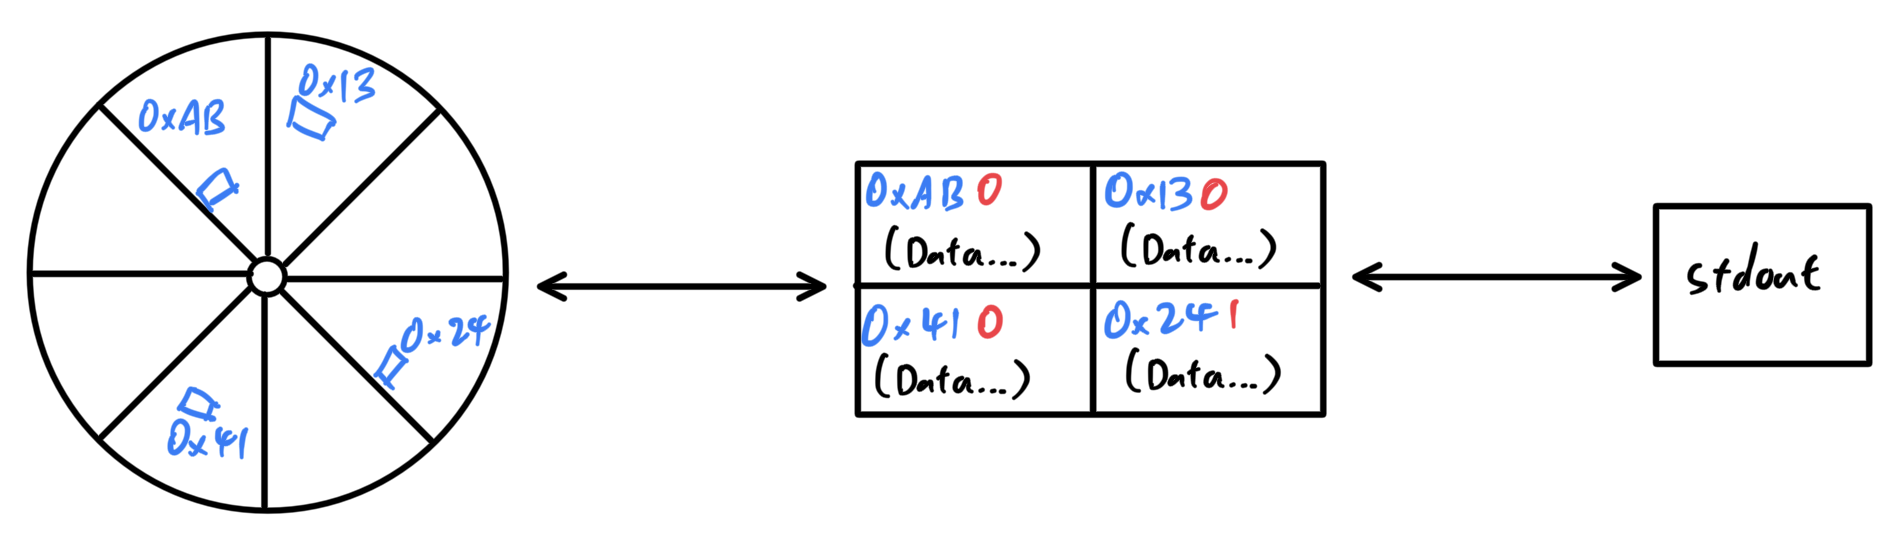
\includegraphics[scale=0.4]{img/disk_memory.png}
        \caption{We store the memory address of the block (blue) and a bit indicating whether it is dirty or not (red). } 
        \label{fig:disk_memory}
      \end{figure}
    \end{definition}

    Therefore, if we want to read $N > M$ blocks, then the first $M$ blocks must be loaded into memory, outputted into stdout, and then the memory must be refilled with the rest of the blocks. If we have updated a block in memory, then we should flush it before overwriting this block in memory.\footnote{idk perhaps we can have a overhead bit indicating whether a block is updated, along with the memory address of this block so it can find it back on the disk.} Replacement strategies won't be covered here. Note that unlike algorithms, which focus on the cost of the algorithm after it is read into memory, we focus on the cost of loading data from the disk into memory. 

    So how should we increase performance? 
    \begin{enumerate}
      \item \textit{Disk Layout}: Keep related things close together, e.g. in the same sector/block, or same track, or same cylinder, or adjacent cylinders. 
      \item \textit{Prefetching}: When fetching a block from the disk, fetch the next block as well since it's pretty likely to access data from the next block. This is basically locality. 
      \item \textit{Parallel I/O}: We can have more heads working at the same time. 
      \item \textit{Disk Scheduling Algorithm}: e.g. the elevator algorithm sorts the cylinders so that you don't go back and forth between cylinders when fetching.  
      \item \textit{Track Buffer}: Read/write one entire track at a time. 
    \end{enumerate}

    Now let's talk about how the actual bytes are stored in memory. 

    \begin{definition}[Row Major Order, NSM]
      We group rows together contiguously in the disk block.\footnote{This is the most standard storage policy.} If we have a relation with schema \texttt{R(INT(4), CHAR(24), INT(4), DOUBLE(8))}, we first store the rows together, with extra space in between since we might append new attributes, and have a tuple of pointers to the start of each row (orange lines). 

      \begin{figure}[H]
        \centering 
        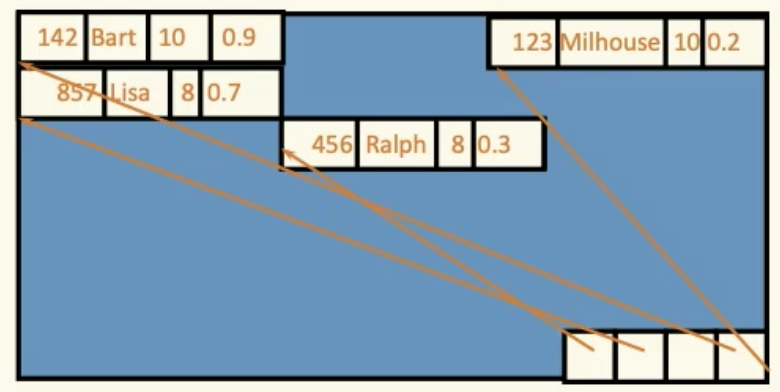
\includegraphics[scale=0.4]{img/row_major.png}
        \caption{} 
        \label{fig:row_major.png}
      \end{figure}
    \end{definition}

    Note that \texttt{VARCHAR} still allocates the same number of bytes, but adds padding. 

    \begin{definition}[Column Major, PAX]
      We group columns together contiguously in the disk block, which allows for optimization since all types are the same and we can just use pointer arithmetic to get every attribute in $O(1)$ time. We split the block into chunks and have metadata of pointers that point to the start of the array for each attribute. 

      \begin{figure}[H]
        \centering 
        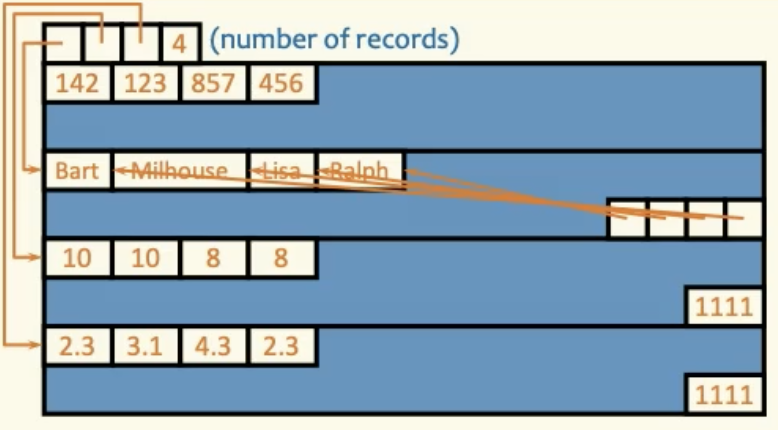
\includegraphics[scale=0.4]{img/column_major.png}
        \caption{} 
        \label{fig:column_major}
      \end{figure}
    \end{definition}

  \subsection{Dense/Sparse and Primary/Secondary Index}

    \begin{definition}[Index vs Search Key]
      Indexes and search keys should be distinguished. They both refer to an attribute of a relation, but are slightly different. 
      \begin{enumerate}
        \item An \textbf{index} is a set of attribute values (e.g. \texttt{uid} of values \texttt{123, 456, 789}) that is a part of our query. 

        \item A \textbf{search key} refers to the attribute on which the index is defined. 
        \begin{lstlisting}
          SELECT * FROM Users WHERE Age = 50; 
        \end{lstlisting}
        \texttt{Age} is the search key, and its search key values may be \texttt{20, 30, 12, 34, 50}. 
      \end{enumerate}
    \end{definition}

    \begin{definition}[Dense vs Sparse Index]
      Sparse and dense just refers to how much an index ``covers'' a disk block. 
      \begin{enumerate}
        \item A \textbf{dense index} means that there is one index entry for each search key value. One entry may point to multiple records
        \item A \textbf{sparse index} means that there is one index entry for each block. Records must be clustered according to the search key as shown below, and this can optimize searching. 
      \end{enumerate}

      \begin{figure}[H]
        \centering 
        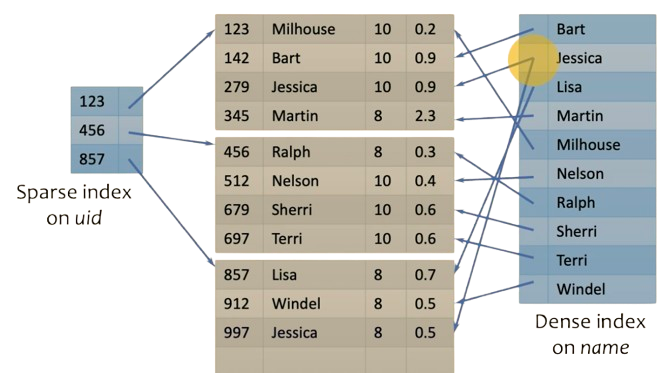
\includegraphics[scale=0.4]{img/dense_sparse.png}
        \caption{The dense index has 10 values, but there are two Jessicas, so it is indeed dense. The sparse index is on the uid, and since the relation is sorted (a more specific form of \textit{clustering}) in the disk, we can use sparse keys.} 
        \label{fig:dense_sparse}
      \end{figure}

      Note that 
      \begin{enumerate}
        \item The sparse index must contain at least the number of blocks, while the dense index must contain at least the number of unique search key values. Since the sparse index is much smaller, we may be able to fit it into main memory and not have to pay the I/O cost. 
        \item A dense index does not require anything on the records, while the sparse requires the data to be clustered. 
        \item Lookup is easy on dense since we can directly see if it exists. For sparse, we must first follow the pointer and scan the block. (e.g. if we wanted to look for 279, we want to look at the address pointed to by 123, and scan down until we hit it or reach a number greater than 279). 
        \item Update is usually easier on sparse indices since we don't need to update the index unless we add a new block. For dense, if we added a new person Muchang, then we would have to add \texttt{Muchang} to the dense index. 
      \end{enumerate}
    \end{definition}

    \begin{definition}[Primary vs Secondary Index]
      Primary and secondary refers to what the index is over. 
      \begin{enumerate}
        \item A \textbf{primary index} is created for the primary key of the relation. Records are usually clustered by the primary key, so this can be sparse. 
        \item A \textbf{secondary index} is any index that is not over a primary key and is usually dense. 
      \end{enumerate}
      In SQL, the \texttt{PRIMARY KEY} declaration automatically creates a primary index, and the \texttt{UNIQUE} declaration creates a secondary index. 
    \end{definition}

    \begin{example}
      You can also create an additional secondary index on non-key attributes. For example, if you think that you will query based on popularity often, you can do 
      \begin{lstlisting}
        CREATE INDEX UserPopIndex ON User(pop); 
      \end{lstlisting}
      which will create a dense index to speed up lookup at the cost of memory. 
    \end{example}

  \subsection{B+ Trees}

    This leads to the problem of the index being too big to fit into a block. In this case, we can just create a sparse index on top of the dense index. This allows us to store a large index across blocks. 
    
    \begin{figure}[H]
      \centering 
      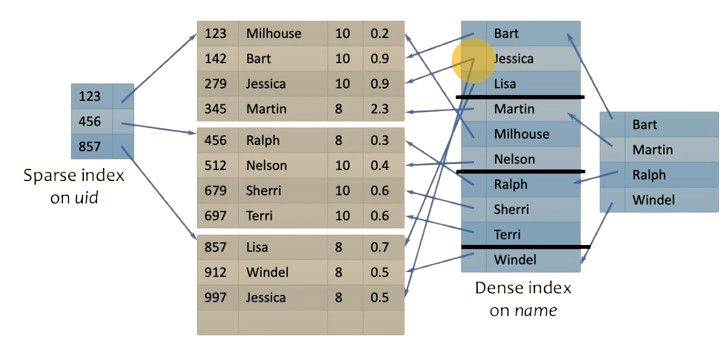
\includegraphics[scale=0.4]{img/too_big.png}
      \caption{} 
      \label{fig:too_big}
    \end{figure}

    If the index is still too big, we store another index on top of that, and we have pretty much a tree. This is called the Index Sequential Access Method (ISAM). 
    
    \begin{example}
      If we want to look up 197 in this tree, we traverse down. 

      \begin{figure}[H]
        \centering 
        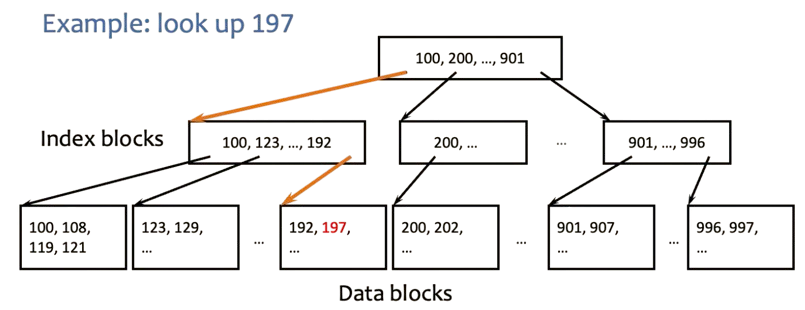
\includegraphics[scale=0.4]{img/isam_lookup.png}
        \caption{} 
        \label{fig:isam_lookup}
      \end{figure}
    \end{example}

    A problem with this method is also a problem with BSTs. If we want to delete 123 and add 107 ten times, then we have an unbalanced binary search tree and this reduces to a linear search. 

    \begin{figure}[H]
      \centering 
      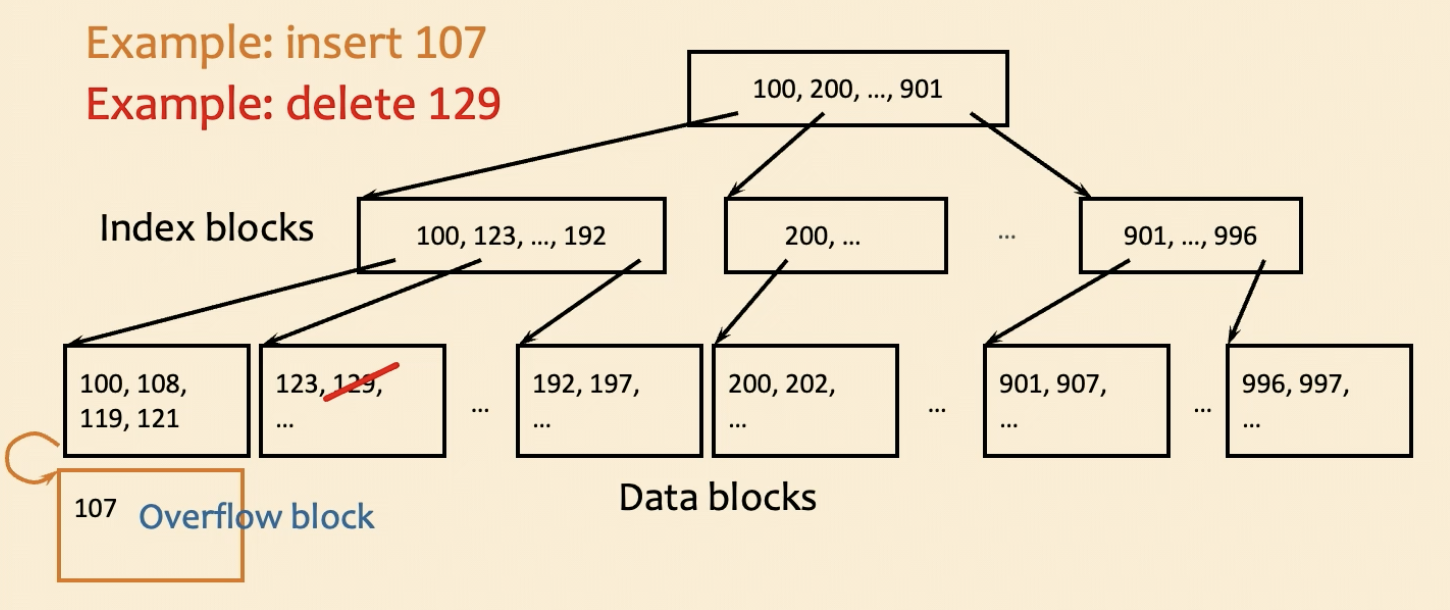
\includegraphics[scale=0.4]{img/isam_problem.png}
      \caption{If this block overflows, then we want to expand this, leading to an unbalanced BST and reducing our search to linear time.} 
      \label{fig:isam_problem}
    \end{figure}
    
    Therefore, this static data structure is not good, and we must use a more flexible one. 

    \begin{definition}[B Tree]
      We look at a generalization of the BST to a B-tree. 

      \begin{figure}[H]
        \centering 
        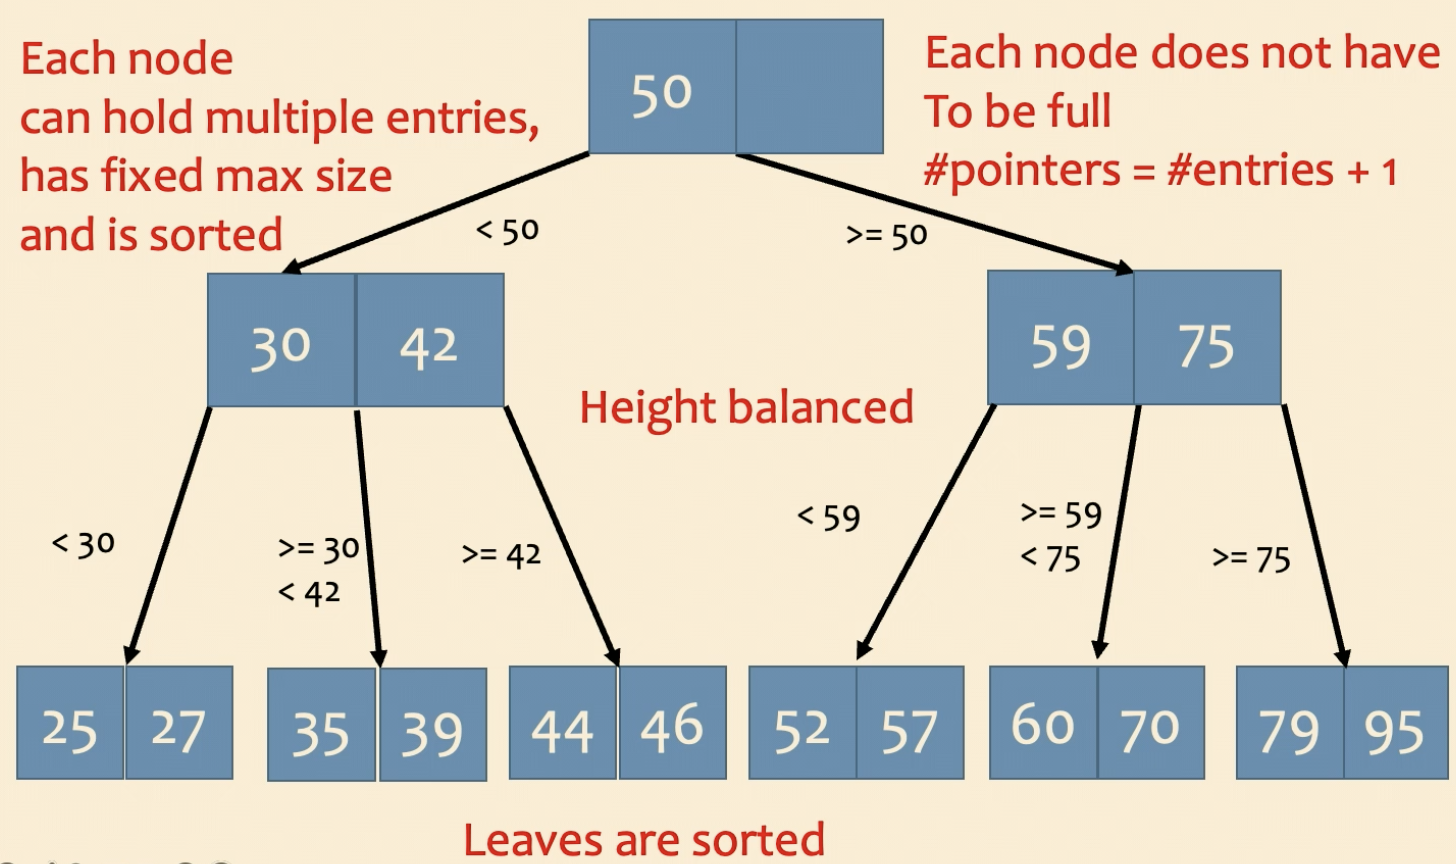
\includegraphics[scale=0.4]{img/b_tree.png}
        \caption{} 
        \label{fig:b_tree}
      \end{figure}
    \end{definition}

    The actual structure that DBMS uses is the B+ tree. 

    \begin{definition}[B+ Tree]
      While in B trees, the non-leaf nodes are also data, the B+ trees divide the nodes into leaf nodes, which represent the data in this data structure, and the non-leaf nodes, which do not represent data but index nodes containing index entries. 

      \begin{figure}[H]
        \centering 
        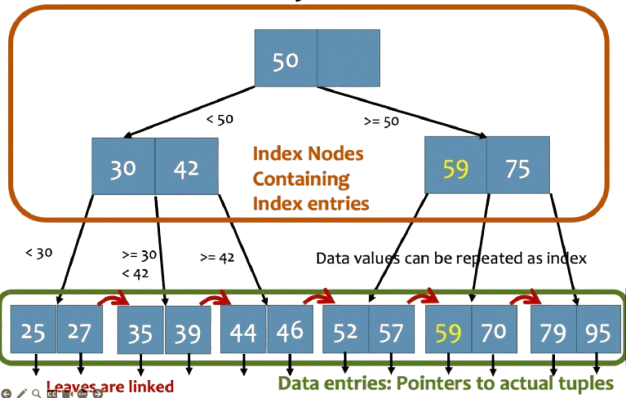
\includegraphics[scale=0.4]{img/bp_tree.png}
        \caption{Note that the 59, which represents both the index and the data value, are repeated. In here, we assume a block size of 2. The leaf nodes are the indices that point to the tuples in the disk/memory. Sometimes, we may store the tuple directly in the nodes, which saves us another level of indirection, but this may cause memory problems if the tuples have too many attributes.} 
        \label{fig:bp_tree}
      \end{figure}

      It has the following constraints: the \textbf{fanout} refers the to maximum number of pointers that can come out of each node. 

      \begin{figure}[H]
        \centering 
        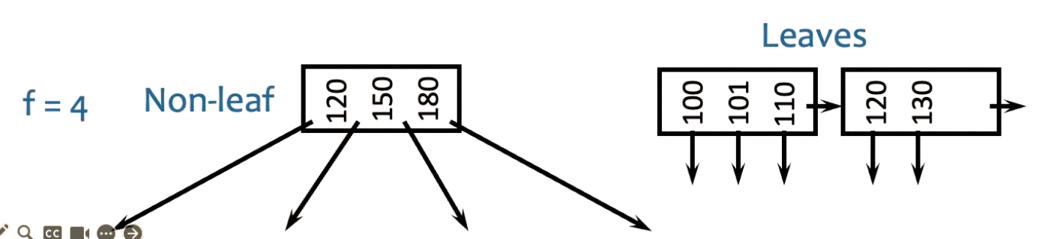
\includegraphics[scale=0.4]{img/fanout.png}
        \caption{With fanout constraint 4, for index nodes, we have 3 values with 4 pointers representing each range. For the leaves, we have 3 pointers to the disk addresses plus 1 pointer to the next node. } 
        \label{fig:fanout}
      \end{figure}

      Therefore, if we have a fanout of $f$, the table shows the constraints. Note that there is a minimum constraint to ensure that the tree is balanced. 

      \begin{figure}[H]
        \centering 
        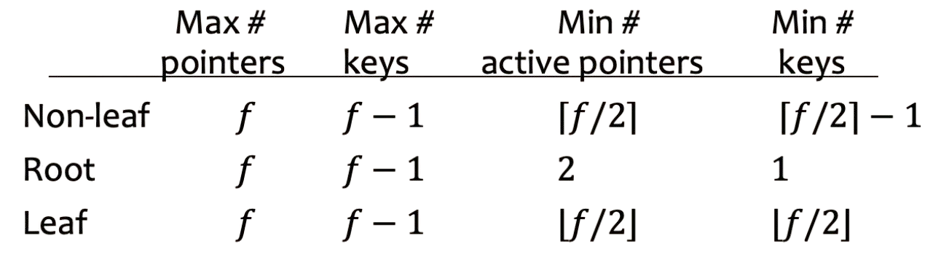
\includegraphics[scale=0.4]{img/chart.png}
        \caption{} 
        \label{fig:chart}
      \end{figure}

      Note that the root is the only node that can store one value. It is special in this way. 
    \end{definition}

    \begin{definition}[Lookup]
      If we query \texttt{SELECT \* FROM R WHERE k = 179;}, we go through the B+ tree's indices and reach the leaf node. From here, we can use the pointer to go to the memory address holding this tuple in memory/disk. If we query \texttt{k = 32}, then we will not find it after reaching \texttt{35}. If we want to query a range \texttt{32 < k < 179}, we start at 32 and use the leaf pointers to go to the next leaf until we hit 179. 

      \begin{figure}[H]
        \centering 
        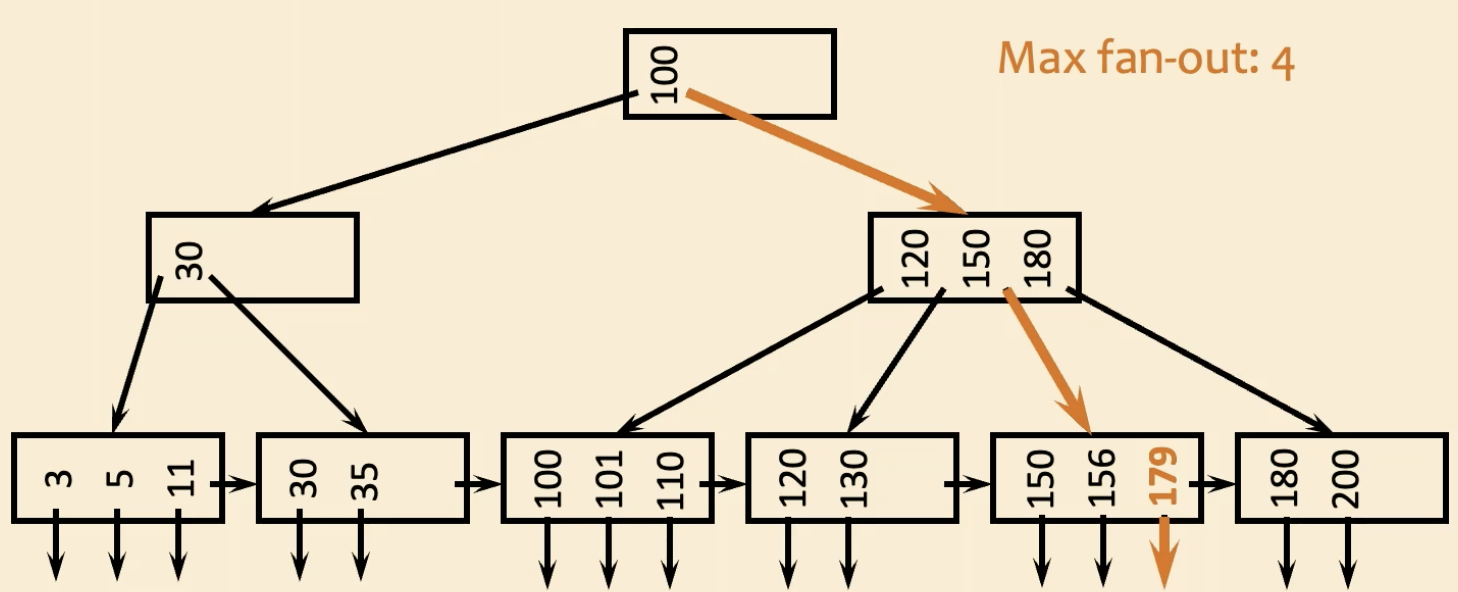
\includegraphics[scale=0.4]{img/fanout_ex.png}
        \caption{} 
        \label{fig:fanout_ex}
      \end{figure}

      In practice, there are much more pointers, so we could start at 179 and go back to 32 if we had backwards pointers. 
    \end{definition}

    Let's see how it is dynamic, i.e. how it changes as we add/delete/modify data. 

    \begin{definition}[Insertion]
      Insertion onto a leaf node having space is easy. 
      
      \begin{figure}[H]
        \centering 
        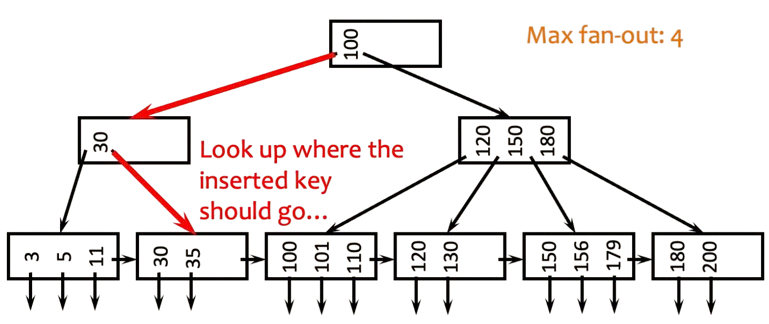
\includegraphics[scale=0.4]{img/insertion_easy.png}
        \caption{Note that to traverse this tree, we had to access 3 blocks of memory since for each block, we had to go to the disk, look up its contents, and retrieve the index of the next block (retrieve the blocks containing (100), (30), and (30, 35)) Then we have to update this block of (30, 35) and flush it. }
        \label{fig:insertion_easy}
      \end{figure}

      When we have a full node, it is more complicated. 
      \begin{enumerate}
        \item Say that we have a full node. We can try to push the rest of the leaf nodes to next node having space, but we are not guaranteed that the neighbors will have space. 

        \begin{figure}[H]
          \centering 
          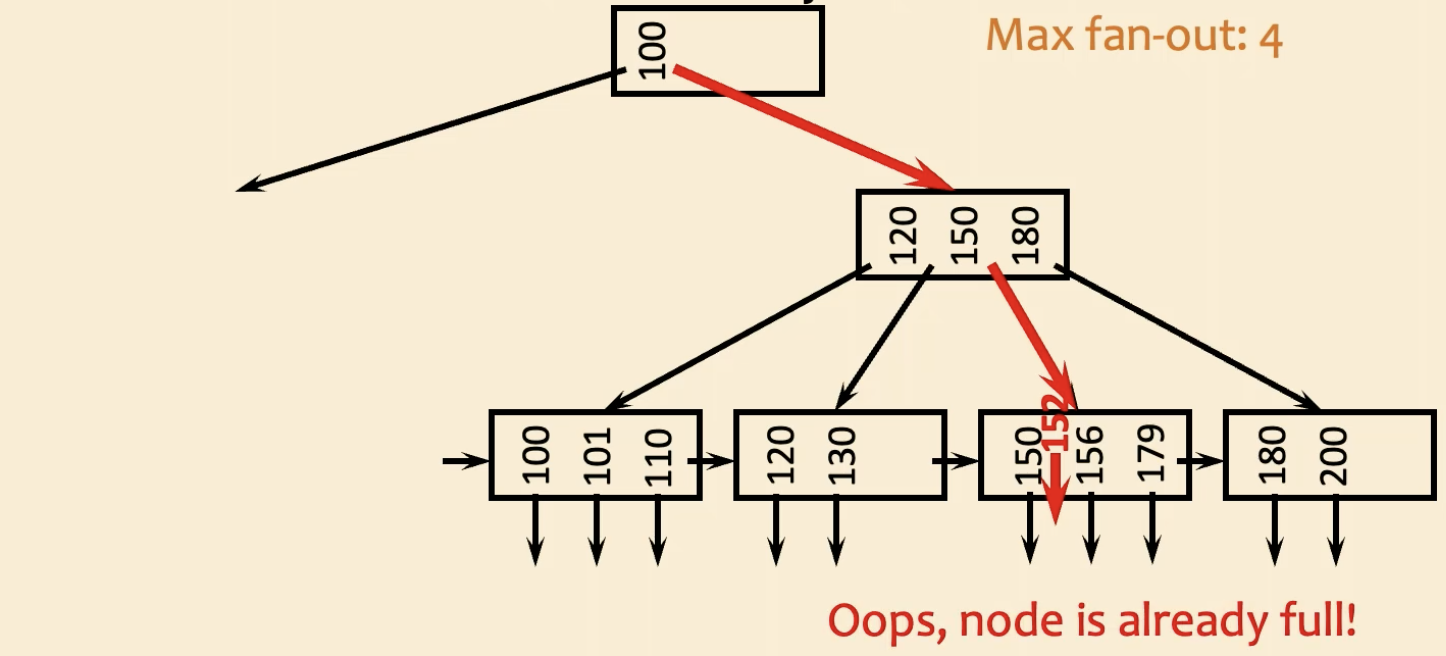
\includegraphics[scale=0.4]{img/insertion_1.png}
          \caption{} 
          \label{fig:insertion_1}
        \end{figure}

        \item We can split the node, called a \textbf{copy-up}. However, this new node now has no pointer. If the parent node is not full, we can just add the pointer and update its value. 

        \begin{figure}[H]
          \centering 
          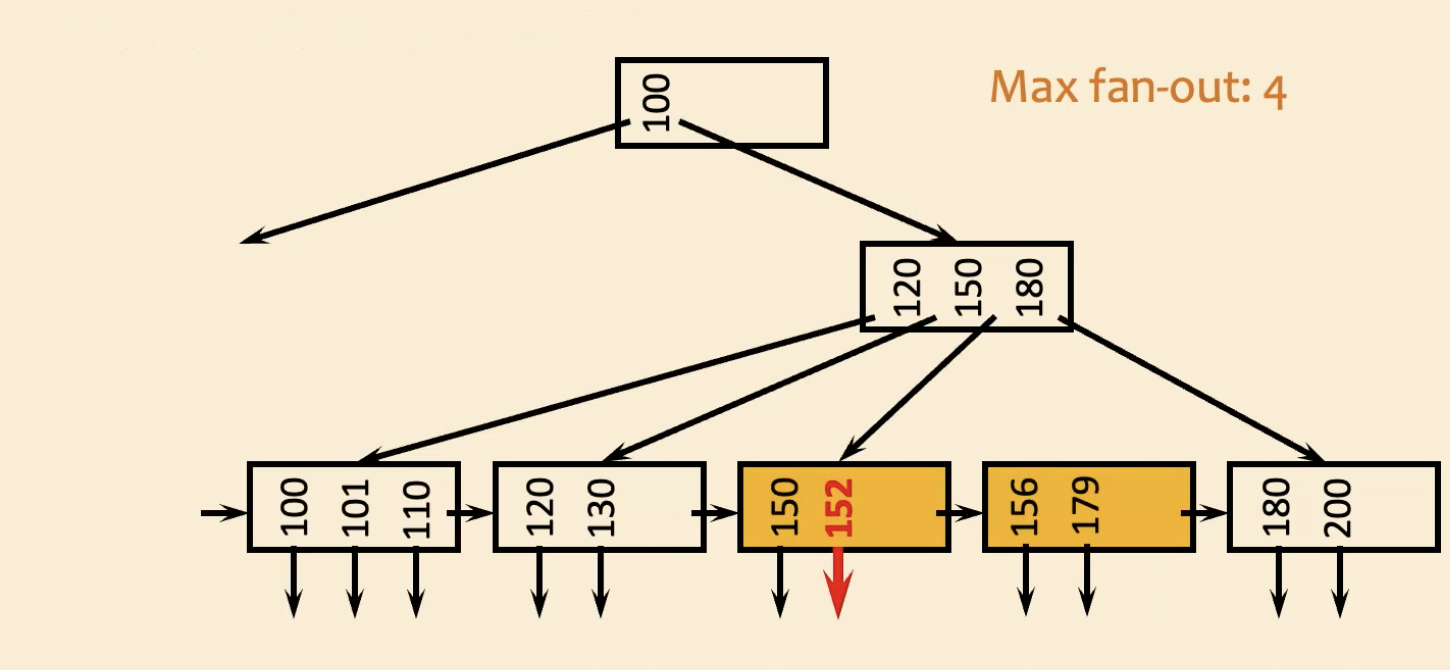
\includegraphics[scale=0.4]{img/insertion_2.png}
          \caption{} 
          \label{fig:insertion_2}
        \end{figure}

        \item If it is full, then we should split the parent node as well. This is called a \textbf{push-up}. 

        \begin{figure}[H]
          \centering 
          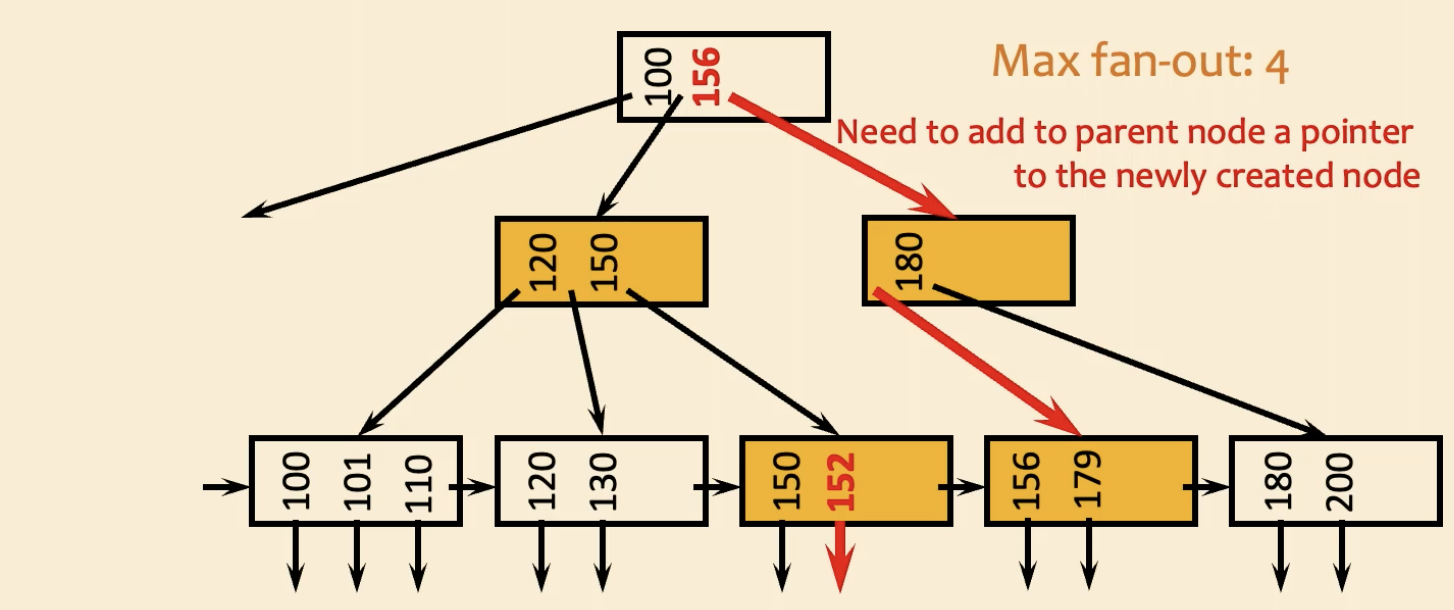
\includegraphics[scale=0.4]{img/insertion_3.png}
          \caption{} 
          \label{fig:insertion_3.png}
        \end{figure}

        \item This means that we have to update the parent of the parent. If the parent is not full, then we simply add it, and if it is full, then we split the parent of the parent, and so on. If we reach the root node, then we just split the root and increase the height of the tree.\footnote{This is rare in practice since the fanout is much greater than 3.}
      \end{enumerate}
    \end{definition}


    \begin{definition}[Deletion]
      Deleting a value is simple if after deletion, the leaf node has at least $f/2$ pointers ($f/2 - 1$ values). 
      
      \begin{enumerate}
        \item If the node has less than $f/2$ pointers, then it is too empty. We can adjust by taking adjacent nodes and moving them from the full nodes to the empty nodes, but this may steal too much from siblings. 

        \begin{figure}[H]
          \centering 
          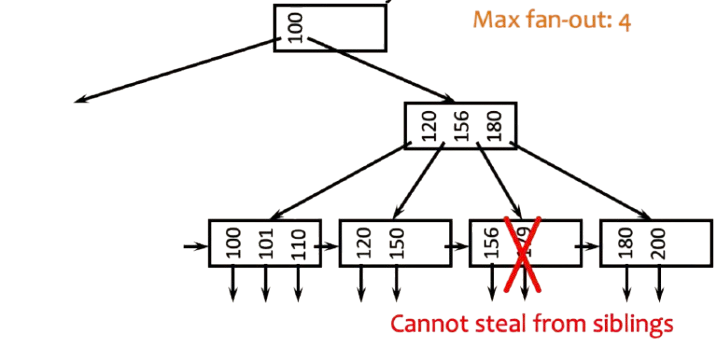
\includegraphics[scale=0.4]{img/deletion_1.png}
          \caption{} 
          \label{fig:deletion_1}
        \end{figure}

        \item The adjacent nodes may be empty as well, and in this case we want to \textbf{coalesce} or merge the nodes together. This results in a dangling pointer, so we delete the pointer and remove a value from the parent node.\footnote{In practice, this is not done every deletion. This reorganizing process can be deferred and the B+ tree property may temporarily not hold.} 

        \begin{figure}[H]
          \centering 
          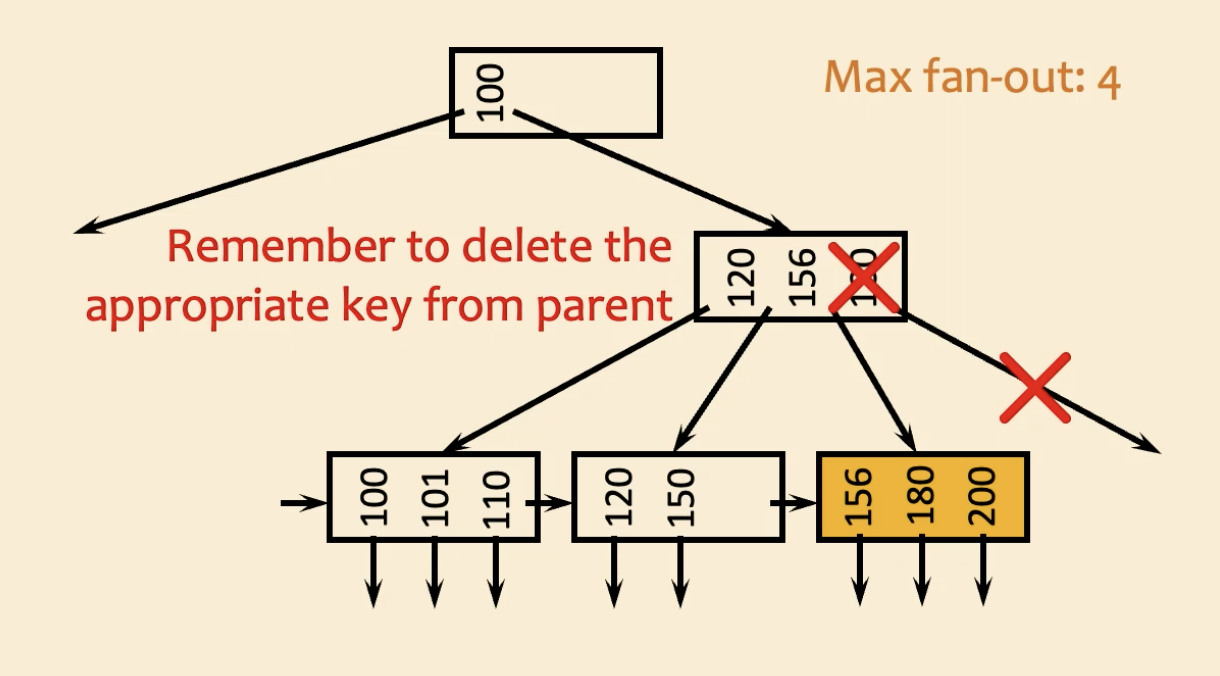
\includegraphics[scale=0.4]{img/deletion_2.png}
          \caption{} 
          \label{fig:deletion_2}
        \end{figure}

        \item We keep doing this until the B+ tree requirements are satisfied or we reach the root, at which point we delete the root node and our B+ tree height decreases by 1. 
      \end{enumerate}
    \end{definition}

    In general, all these operations have similar runtimes: 
    \begin{enumerate}
      \item They require us to go to the bottom of the tree, so it is $h$ operations, where $h$ is the height. 
      \item We also maybe have $+1$ or $+2$ to manipulate the actual records, plus $O(h)$ for reorganization like we saw before (which is rare if $f$ is large). 
      \item Minus 1 if we cache the root in memory, which can be decreased even further if we cache more blocks. 
    \end{enumerate}
    
    The actual size of $h$ is roughly $\log_{f/2} {N}$, where $N$ is the number of records. $f$ is the fanout, but the B+ tree properties guarantee that there are at least $f/2$ pointers, so it is $\log_{f/2} N$ at worst and $\log_{f} N$ at best. $f$ is very large usually so this is quite good. 

    The reason we use B+ trees rather than B trees is that if we store data in non-leaf nodes, this decreases the fanout $f$ and increases $h$. Therefore, records in leaves require more I/Os to access. 

  \subsection{Clustered vs Unclustered Index}

    \begin{definition}[Clustered vs Unclustered Index]
      If the order of the data records in a file is the same as or close to the order of data entries in an index (basically means sorted with respect to the order on the relation), then it is \textbf{clustered}, and otherwise \textbf{unclustered}. 

      \begin{figure}[H]
        \centering 
        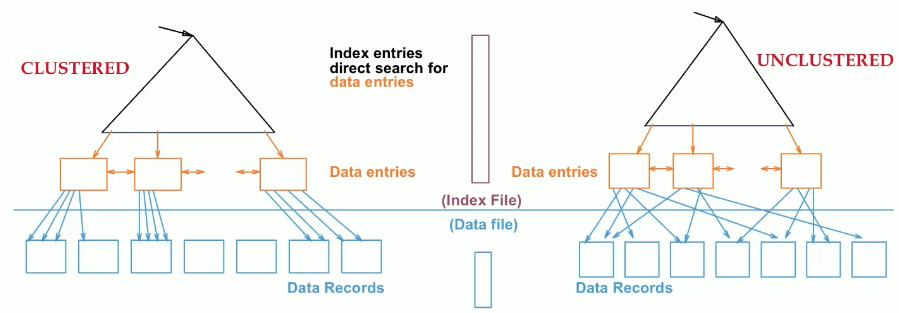
\includegraphics[scale=0.4]{img/clustered_vs_unclustered.png}
        \caption{Even if the data entries (leaf nodes) are sorted, the memory addresses of the blocks on disk that they point to may not be sorted.} 
        \label{fig:clustered_vs_unclustered}
      \end{figure}

      Note that the B+ tree is still a search tree! It is sorted. The clustered is a property of the data (blue squares). 
    \end{definition}

    The performance can really depend on whether the index is clustered or unclustered. 

    \begin{example}[Possible Final Exam Question]
      Assume that we have the query \texttt{SELECT \* FROM User WHERE age = 50;} with the following assumptions: 
      \begin{enumerate}
        \item Assume 12 Users with \texttt{age = 50}. 
        \item Assume one data page (block) can hold 4 User tuples (so $f = 5$). 
        \item Suppose searching for data entry requires 3 IOs in a B+ tree, which contain pointers to the data records (so $h = 3$). 
      \end{enumerate}

      If the index is clustered, then we can just traverse down the B+ tree to get to the leaf node containing the value 50. 
      \begin{enumerate}
        \item We have a cost of 3 to traverse down the tree to access the index pages which show the memory addresses of the tuples on disk. 

        \item Then, we will find entries and we want to find the cost to access the data pages. There are 12 Users, and for every address, we load the entire block in memory, which will retrieve the other users of age 50 (since this is clustered). At best, we will retrieve 3 blocks (of 4 tuples each) and at worst, due to block overlap, we will retrieve 4 blocks and read the rest from memory. This gives us a cost of $+3$ or $+4$. 
      \end{enumerate}
      The total cost is 6. If the index is unclustered, then we are not guaranteed that the data with values 50 will be contiguous, so we will in the worst case have to look at 12 different blocks, leading to a total cost of $3 + 12 = 15$. 
    \end{example}

  \subsection{Hash and Composite Index}

    \begin{definition}[Hash Index]
      So far, we have used tree indices. However, an alternative is to use a \textbf{hash index} which hashes the search keys for comparison. Hash indices can only handle equality queries. 
      \begin{enumerate}
        \item \texttt{SELECT * FROM R WHERE age = 5; } (requires hash index on \texttt{(age)})
        \item \texttt{SELECT * FROM R, S WHERE R.A = S.A; } (requires hash index on \texttt{R.A} or \texttt{S.A})
        \item \texttt{SELECT * FROM R WHERE age = 5 AND name = 'Bob' } (requires hash index on \texttt{(age, name)})
      \end{enumerate}
      They are more amenable to parallel processing but \textit{cannot handle range queries or prefixes}, e.g. \texttt{SELECT * FROM R WHERE age >= 5;}. Its performance depends on how good the hash function is (whether it distributes data uniformly and whether data has skew). 
    \end{definition}

    \begin{definition}[Composite Index]
      We've looked at queries in the form \texttt{SELECT \* FROM User WHERE age = 50;}, but what if there are multiple conditions. For example, if we have 
      \begin{lstlisting}
        SELECT * FROM User WHERE age >= 25 AND name = 'B'; 
      \end{lstlisting}
      then we can do a couple things: 
      \begin{enumerate}
        \item We have the index on \texttt{(age)}, at which point the leaf nodes will look something like 
          \begin{equation}
            25, 25, 25, 26, 26, 28, 29, 29
          \end{equation}
          We traverse through all the addresses in these leaf nodes and find the ones with name \texttt{B}. 

        \item If we have a \textbf{composite index} on \texttt{(age, name)}, then our leaf nodes will sort them as 
          \begin{equation}
            (25, A), (25, A), (25, B), (26, A), (26, C), (28, B), (29, A), (29, C)
          \end{equation}

        \item If we index on \texttt{(name, age)}, then our leaf nodes will sort them as 
          \begin{equation}
            (A, 25), (A, 25), (A, 26), (A, 29), (B, 25), (B, 28), (C, 26), (C, 29)
          \end{equation}
          Note that if we had the query \texttt{SELECT \* FROM R WHERE age >= 25}, then this sorting would not help since we do not prioritize ordering by age. So we cannot use tree indexing over name, age for this query. 
      \end{enumerate}
    \end{definition}

    \begin{example}
      Therefore, given a query, there are certain indices that we can use or cannot use for it.
      \begin{enumerate}
        \item If we have a query \texttt{A >= 5}, 
          \begin{enumerate}
            \item Can use hash index in general.  
            \item Can use tree index in general. 
          \end{enumerate}

        \item If we have query \texttt{A >= 5}, 
          \begin{enumerate}
            \item Can use tree with index (A). 
            \item Can use tree with index (A, B). 
            \item Cannot use tree with index (B, A) since A is not prefix. 
          \end{enumerate}

        \item If we have query \texttt{A = 5},
          \begin{enumerate}
            \item Can use hash with index (A). 
            \item Can use tree with index (A). 
            \item Cannot use hash with index (A, B) since hashing this tuple does not allow us to compare to A or retrieve it. It is one-way and pseudo-random.   
            \item Can use tree with index (A, B). 
          \end{enumerate}

        \item If we have \texttt{A = 5 AND B = 7}, 
          \begin{enumerate}
            \item Can use hash with index (A, B). 
          \end{enumerate}
      \end{enumerate}
    \end{example}

    Each index has its pros and cons, so why not just use both tree and hash indices? The problem is that when we modify a relation on the disk, we need to update the index as well. Therefore, having too many indices requires us to update more and takes more disk space. 

    Okay, so we can't use too many indices, but are indices \textit{always} better than table scans? Not exactly. 
    
    \begin{example}[Table Scans Wins]
      Consider $\sigma_{A > v} (R)$ and a secondary, non-clustered index on $R(A)$ with around 20\% of $R$ satisfying $A > v$ (could happen even for equality predicates). We need to follow pointers to get the actual result tuples. 
      \begin{enumerate}
        \item IOs for scan-based selection is simply $B(R)$ (where we can retrieve multiple tuples in this block), while 
        \item IOs for index-based selection is the lookup-cost (to traverse down the tree) plus $0.2 |R|$ (since for each tuple, we do a IO lookup, retrieve it, and then have to retrieve the next tuple which is likely not in the same block)
      \end{enumerate}
      So table scan wins if a block contains more than 5 tuples since we might as well grab everything rather than look them up one by one. 
    \end{example}

    Thankfully, the query optimizer will make these decisions for you. 

  \subsection{Index Only Plans}

    \begin{definition}[Index-Only Plans]
      There are queries that can be answered only by accessing the index pages and not the data pages, known as \textbf{index-only plans}. For index-only plans, clustering is not important since we are looking only at the leaf nodes at most. Therefore, we only need to compute the I/O cost of traversing the tree and not to access data. 

      For equality, we can just compute the number of tuples in the index pages where the equality condition is satisfied. For ranges, we may need to traverse the leaf nodes, which will lead to additional I/O cost to retrieve the leaf index pages. 
    \end{definition}

    \begin{example}[Index Only Queries]
      If we look at the following query 
      \begin{equation}
        \pi_A (\sigma_{A > v} (R))
      \end{equation}
      we see that we only care about the value of $A$ and not the rest of the tuples, so we only need to look at the index pages and not the data itself. 
    \end{example}

    \begin{example}[Primary Index Clustered According to Search Key]
      If we have a primary index, in most cases the actual records are also stored in the index pages/leaf nodes. If they are clustered according to attribute $A$, then one lookup can lead to all result tuples in their entirety. You can just hit a leaf and grab your records as you walk along the leaves. 
    \end{example}

    \begin{example}[Other Index-Only Queries]
      For example, if we just wanted to look at the count of users with age 50, then we don't need the data. We can just look at the number of values in the leaf nodes of the B+ tree with this value. 
      \begin{lstlisting}
        SELECT E.do COUNT(*) 
        FROM Emp E 
        GROUP BY E.dno;
      \end{lstlisting}

      If we have an index on \texttt{(E.dno, E.sal)}, then the two queries are also index-only plans. However, if we index on \texttt{(E.dno)}, then we need to retrieve \texttt{E.sal} on the data page, incurring more cost. 

      \noindent\begin{minipage}{.5\textwidth}
      \begin{lstlisting}[]{Code}
        SELECT E.dno, MIN(E.sal) 
        FROM Emp E 
        GROUP BY E.dno; 
      \end{lstlisting}
      \end{minipage}
      \hfill
      \begin{minipage}{.49\textwidth}
      \begin{lstlisting}[]{Output}
        SELECT AVG(E.sal) 
        FROM Emp E 
        GROUP BY E.dno;
      \end{lstlisting}
      \end{minipage}
    \end{example}

    \begin{example}[Halloween Problem]
      The Halloween problem refers to a phenomenon in databases where an update operation causes a change in the physical location of a row, potentially allowing the row to be visited again later in the same update operation. Look at the update. 
      \begin{lstlisting}
        UPDATE Payroll 
        SET salary = salary * 1.1 
        WHERE salary <= 25000;
      \end{lstlisting}
      This caused everyone to have a salary of $25000+$. This is because when we updated someone with salary of say $1000$, it went to $1100$ and is moved further right in the B+ tree. Therefore, this is revisited again is increased again in the same update. To fix this, we could update the values in reverse, from the rightmost leaf node to the leftmost one so that increasing values are visited once. Or we can just create a to-do/done list that keeps track of which ones have been updated. 
    \end{example}

\section{Query Processing}

    To set up some notation, let $B(R)$ represent the number of disk blocks that relation $R$ takes up, and say $M$ is the number of blocks available in our memory. We start off with some simple operations. 

    \begin{example}
      Suppose we have relation $R$ with $|R| = 1000$ and each block can hold 30 tuples. Then $B(R) = \lceil 1000 / 30 \rceil = 34$, or 35 if there is overlap. 
    \end{example}

    \begin{example}[Cost of Querying Everything]
      If we do \texttt{SELECT * FROM R}, then 
      \begin{enumerate}
        \item we are at most retrieving $B(R)$ pages from disk to memory, so our IO cost is $B(R)$. 
        \item Our memory cost is 2 pages since we take each page, load it to memory, and put the answer in the output page. The next page (if any) can overwrite the previously loaded page. 
      \end{enumerate}
      We can stop early if we lookup by key. Remember that this is not counting the cost of writing the result out. 
    \end{example}

  \subsection{External Merge Sort}

    Now let's talk about processing of queries, namely how sorting works in a database system, called \textbf{external merge sort}. In an algorithm course, we know that the runtime is $O(n \log{n})$, but this is for CPU comparisons where the entire list is loaded in memory. This is extremely trivial in comparison to the IO commands we use in databases, so we will compute the runtime of sorting a relation by an attribute in terms of IO executions. 

    \begin{definition}[External Merge Sort]
      The problem is that we want to sort $R$ but $R$ does not fit in memory. We divide this algorithm into passes. 
      \begin{enumerate}
        \item Pass 0: Read $M$ blocks of $R$ at a time, sort them, and write out a level 0 run. 
        \item Pass 1: Merge $M-1$ level 0 runs at a time, and write out a level 1 run. 
        \item Pass 2: Merge $M-1$ level 1 runs at a time, and write out a level 2 run. 
        \item Final pass produces one sorted run. 
      \end{enumerate}

      \begin{figure}[H]
        \centering 
        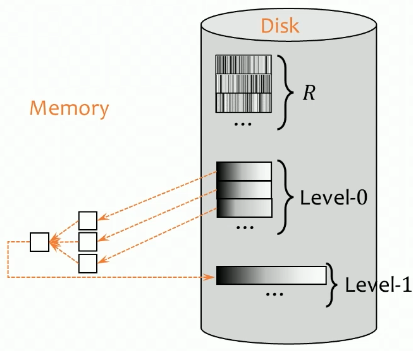
\includegraphics[scale=0.4]{img/merge.png}
        \caption{} 
        \label{fig:merge}
      \end{figure}

      To compute the cost, we know that 
      \begin{enumerate}
        \item in pass 0, we read $M$ blocks of $R$ at a time, sort them, and write out a level 0 run, so there are 
          \begin{equation}
            \lceil B(R) / M \rceil
          \end{equation}
          level 0 sorted runs, or passes. 

        \item in pass $i$, we merge $M-1$ level $(i-1)$ runs at a time, and write out a level $i$ run. We have $M-1$ memory blocks for input and $1$ to buffer output, so 
          \begin{equation}
            \text{Num. of level i runs} = \bigg\lceil \frac{\text{Num. of level (i-1) runs}}{M-1} \bigg\rceil 
          \end{equation}

        \item The final pass produces 1 sorted run. 
      \end{enumerate}

      Therefore, the number of passes is 
      \begin{equation}
        \bigg\lceil \log_{M-1} \Big\lceil \frac{B(R)}{M} \Big\rceil \bigg\rceil + 1
      \end{equation}
      and the number of IOs is $2 B(R)$ since each pass reads the entire relation once and write it once. The memory requirement is $M$ (as much as possible). 
    \end{definition}

    \begin{example}
      Assume $M = 3$, with each block able to hold at most 1 number. Assume that we have an input (relation) 
      \begin{equation}
        1, 7, 4, 5, 2, 8, 3, 6, 9
      \end{equation}
      Then we go through multiple passes. 
      \begin{enumerate}
        \item Pass 0 will consist of 3 runs. You load each of the 3 numbers in memory and sort them.  
          \begin{align}
            1, 7, 4 & \mapsto 1, 4, 7 \\ 
            5, 2, 8 & \mapsto 2, 5, 8 \\ 
            9, 6, 3 & \mapsto 3, 6, 9
          \end{align}

        \item Pass 1. You merge them together by first taking 1 and 2, loading them in memory, and then comparing which one should go first. Once 1 is outputted, then the next number 4 overwrites 1 in memory, and then 2 is outputted, and so on. 
          \begin{align}
            & 1, 4, 7 + 2, 5, 8 \mapsto 1, 2, 4, 5, 7, 8 \\ 
            & 3, 6, 9
          \end{align}

        \item Pass 2. Merges the final two relations. 
          \begin{align}
            1, 2, 3, 4, 5, 7, 8 + 3, 6, 9 \mapsto 1, 2, 3, 4, 5, 6, 7, 8, 9
          \end{align}
      \end{enumerate}
      Therefore, pass 0 uses all $M$ pages to sort, and after that, when we merge, we only use $M-1$ pages to merge the inputs together and $1$ page for the output. 
    \end{example}

    Some performance improvements include: 
    \begin{enumerate}
      \item \textit{Double Buffering}. You allocate an additional block for each run, and while you are processing (merging the relations in memory), you run the IO concurrently and store it in the new block to save some time. 
      \item \textit{Blocked IO}. Instead of reading/writing one disk block at a time, we can read/write a bunch of them in clusters. This is sort of like parallelization where you don't output just one block, but multiple blocks done from multiple processing. 
    \end{enumerate}
    The problem with both of these is that we have smaller fan-in, i.e. more passes. Since we are using more blocks per run than we have, we can look at fewer runs at once. 

  \subsection{Nested Loop Joins} 

    Note that there are many ways to process the same query. We can in the most basic sense just scan the entire relation in disk. We can sort it. We can use a tree or hash index, and so on. All have different performance characteristics and make different assumptions about the data, so the choice is really problem-dependent. What a DBMS does is implements all alternatives and let the \textbf{query optimizer} choose at runtime. 

    \begin{definition}[Nested Loop Join]
      Let's look at a brute force method of a theta join, called \textbf{nested-loop} join. If we run $R \bowtie_p S$, we do a nested for loop: 
      \begin{enumerate}
        \item For each block of $R$ and for each $r$ in the block, we look at each block of $S$ 
        \item For each $s$ in the block, we output $rs$ is $p$ evaluates to true over $r$ and $s$.  
      \end{enumerate}
      In here, $R$ is called the outer table and $S$ the inner table. The number of IOs is 
      \begin{equation}
        B(R) + |R| \cdot B(S)
      \end{equation}
      since we need $B(R)$ to load $R$, and for every tuple, we run through all of $S$. The memory requirement is $3$ since we need 1 block to buffer $R$, 1 to buffer $S$, and 1 output block which acts as a buffer before we write to disk or stdout.\footnote{This is basically a buffer block where if it is filled, it is automatically flushed to disk.}
    \end{definition} 

    This is clearly not efficient since it requires a lot of IOs. We can make a slight improvement. 

    \begin{definition}[Block Based Nested Loop Join]
      For each block in $R$ and for each block in $S$, we try to basically do as much as we can with these two blocks. That is, we take a look at all $r, s \in R, S$ and see if $p$ evaluates to true. The IO is therefore 
      \begin{equation}
        B(R) + B(R) \cdot B(S)
      \end{equation}
      This is because for each block of $R$, we go through all blocks of $S$ and look through all pairwise tuples. The memory requirement is still $3$. 
    \end{definition}

    We can use more memory by basically stuffing the memory with as much of $R$ as possible, stream $S$ by, and join every $S$ tuple with all $R$ tuples in memory. Therefore, the IO cost can be decreased to 
    \begin{equation}
      B(R) + \bigg\lceil \frac{B(R)}{M-2} \bigg\rceil \cdot B(S) \approx B(R) \cdot B(S) / M
    \end{equation}
    You want to pick the bigger table as $R$ since you want the smaller table $S$ to be loaded/streamed in multiple times. 

    \begin{definition}[Index Nested Loop Join]
      If we want to compute $R \bowtie_{R.A = S.B} S$, the idea is to use the value of $R.A$ to probe the index on $S(B)$. That is, for each block of $R$, we load it into memory, and for each $r$ in the block, we use the index on $S(B)$ to retrieve $s$ with $s.B = r.A$, and output $rs$. 

      The IO runtime, assuming that $S$ is unclustered and secondary, is 
      \begin{equation}
        B(R) + |R| \cdot (\mathrm{index lookup}) 
      \end{equation}
      Since typically the cost of an index lookup is 2-4 IOs, it beats other join methods mentioned later if $|R|$ is not too big. Since this does not scale at all with $S$, it is better to pick $R$ to be the smaller relation. The memory requirement as with other operations is $3$ blocks. 
    \end{definition}

  \subsection{Merge Sort Joins}

    \begin{definition}[Sort-Merge Join] 
      A clever way is to first sort $R$ and $S$ by their join attributes, and then merge. Given that the first tuples in sorted $R, S$ is $r, s$, we do repeat until one of the $R$ or $S$ is exhausted. 
      \begin{enumerate}
        \item If $r.A > s.B$, then $s =$ next tuple in $S$ 
        \item Else if $r.A < s.B$, then $r =$ next tuple in $R$. 
        \item Else output all matching tuples and $r, s$ = next in $R, S$, which is basically a nested loop. 
      \end{enumerate}
      This means that the IOs is really 
      \begin{equation}
        \text{sorting} + 2 B(R) + 2 B(S)
      \end{equation}
      which is worst case $B(R) \cdot B(S)$ when everything joins. Note that after sorting them, we must write them back to disk (which is usually the case if we can't fit the sorted relation in memory), which is $B(R) + B(S)$. Then we must load these sorted blocks back into memory, which takes an additional $B(R) + B(S)$. 

      To further optimize this, we can integrate the join with the merging step. We basically want to combine join with the (last) merge phase of merge sort. The runs are merging together, and then in memory we join them. 

      \begin{figure}[H]
        \centering 
        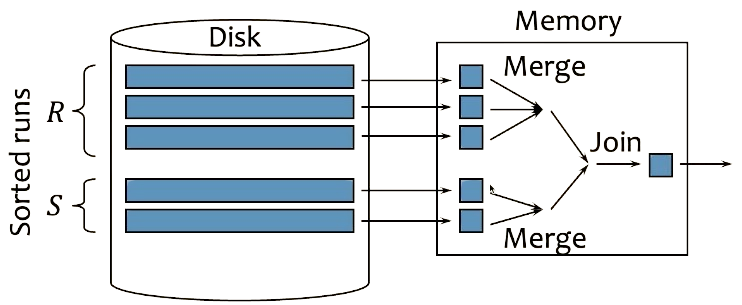
\includegraphics[scale=0.4]{img/smj_optim.png}
        \caption{Sorting: produce sorted runs for $R$ and $S$ such that there are fewer than $M$ of them total. Then in merge and join, we merge the runs of $R$, merge the runs of $S$, and merge-join the result streams as they are generated!} 
        \label{fig:smj_optim}
      \end{figure}

      To analyze the runtime, if SMJ completes in two passes, then the IOs is really cheap. 
      \begin{equation}
        3 ( B(R) + B(S)) 
      \end{equation}
      As for memory, we must have enough memory to accomodate one block from each run, so 
      \begin{equation}
        M > \bigg\lceil \frac{B(R)}{M} \bigg\rceil + \bigg\lceil \frac{B(R)}{M} \bigg\rceil \text{ or roughly } M > \sqrt{B(R) + B(S)}
      \end{equation}
      If SMJ cannot complete in 2 passes, then we repeatedly merge to reduce the number of runs as necessary before the final merge and join. 
    \end{definition}

    \begin{example}
      Look at the following example, by the time we got to the first $3$, we can't just increment the pointers for both relations. We must scan through all of the tuples of A with value 3 and all those in B with value 3 and do a nested loop to join them. 
      
      \begin{figure}[H]
        \centering 
        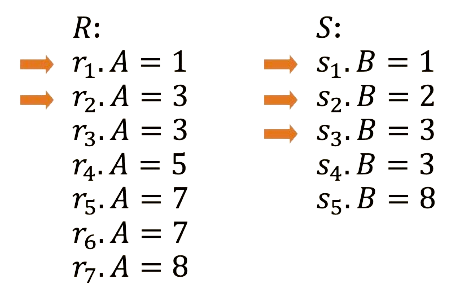
\includegraphics[scale=0.4]{img/nested_loop.png}
        \caption{} 
        \label{fig:nested_loop}
      \end{figure}
    \end{example}

    \begin{definition}[Zig Zag Join using Ordered Indices]
      To compute $R \bowtie_{R.A = S.B} S$, the idea is to use the ordering provided by the indices on $R(A)$ and $S(B)$ to eliminate the sorting step of merge-join. The idea is similar to sort-merge join. We start at the leftmost leaf node of both indices of $R$ and $S$, and traverse (right) through the leaves, querying both of the data at leaf $a$ in $R$ and $b$ in $S$ if the leaf values are equal. 

      Note that we don't even have to traverse through all leaves. If we find that a key is large, we can just start from the root node to traverse, possibly skipping many keys that don't match and not incurring all those IO costs. This can be helpful if the matching keys are distributed sparsely.

      \begin{figure}[H]
        \centering 
        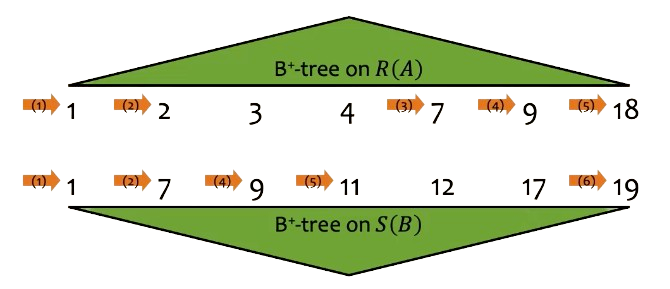
\includegraphics[scale=0.4]{img/zig_zag.png}
        \caption{We see that the B+ tree of $B$ has value $7$ while that of $A$ has value $2$. Rather than traversing $2 \mapsto 3 \mapsto 4 \mapsto 7$, we can just traverse to $7$ from the root node of $A$. This can give us a stronger bound. } 
        \label{fig:zig_zag}
      \end{figure}
    \end{definition}

  \subsection{Other Sort Based Algorithms}

    The set union, intersection, difference is pretty much just like SMJ. 

    For duplicate elimination, you simply modify it so that during both the sort and merge steps, you eliminate duplicates if you find any. 

    For grouping and aggregation, you do external merge sort by the group-by columns. The trick is you produce ``partial'' aggregate values in each run and combine them using merge. 

  \subsection{Hashing Based Algorithms} 

    \begin{definition}[Hash Join]
      Let's start off with \textbf{hash joining}: $R \bowtie_{R.A = S.B} S$. 
      The main idea is that we want to partition $R$ and $S$ by hashing (using a hash function that maps to $M-1$ values) their join attributes and then consider corresponding partitions (that get mapped to the same hash value) of $R$ and $S$. If $r.A$ and $s.B$ get hashed to the same number, they might join, and if they don't, then they definitely won't join. The figure below nicely visualizes this. 
    
      \begin{figure}[H]
        \centering 
        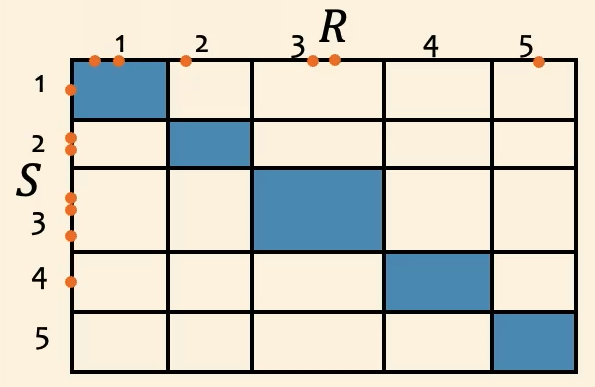
\includegraphics[scale=0.4]{img/hash_join.png}
        \caption{Say that the orange points represent the hashed values of $r.A$ and $s.B$ for $r, s \in R, S$. The nested loop considers all slots (all pairs of orange points between $R$ and $S$), but hash join considers only those along the diagonal. } 
        \label{fig:hash_join}
      \end{figure}

      Then, in the \textbf{probing phase}, we simply read in each partition (the set of tuples that map to the same hash) of $R$ into memory, stream in the corresponding partition of $S$, compare their \textit{values} (not hashes since they are equal), and join if they are equal. If we cannot fit in a partition into memory, we just take a second hash function and hash it again to divide it into even smaller partitions (parallels merge-sort join). 

      \begin{figure}[H]
        \centering 
        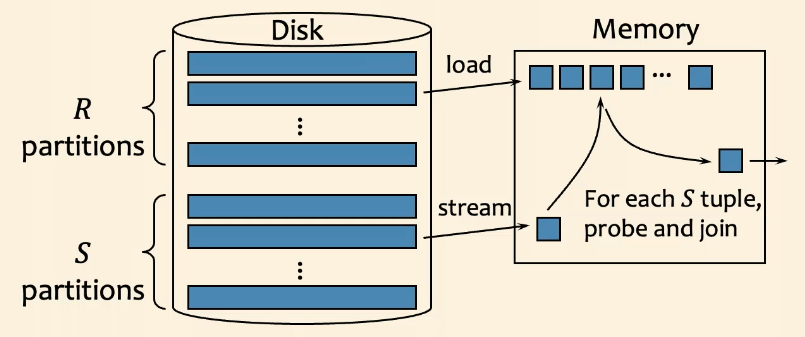
\includegraphics[scale=0.4]{img/hash_join2.png}
        \caption{} 
        \label{fig:hash_join2}
      \end{figure}

      Therefore, if the hash join completes in two passes, the IO runtime is 
      \begin{equation}
        3 ( B(R) + B(S)) 
      \end{equation}
      which is similar to merge-sort join. As for the memory requirement, let's first assume that in the probing phase, we should have enough memory to fit one partition of $R$, i.e. $M-1 > \lceil B(R) / (M-1) \rceil$, so solving for it roughly gives $M > \sqrt{B(R)} + 1$. We can always pick $R$ to be the smaller relation, so roughly 
      \begin{equation}
        M > \sqrt{\min\{ B(R), B(S)\}} + 1
      \end{equation}
    \end{definition}

    To compare hash join and SMU, note that their IOs are the same, but for memory requirements, hash join is lower, especially when the two relations have very different sizes. 
    \begin{equation}
      \sqrt{\min\{B(R), B(S)\}} + 1 < \sqrt{B(R) + B(S)}
    \end{equation}
    Some other factors include the quality of the hash (may not generate evenly sized partitions). Furthermore, hash join does not support inequality joins unlike SMJ, and SMJ wins if either $R$ and/or $S$ is already sorted. SMJ also wins if the result needs to be in sorted order. 

    Sometimes, even block nested loop join may win in the following cases. 
    \begin{enumerate}
      \item if many tuples join (as in the size of the join is $|S| \cdot |R|$) since we are doing unnecessary processing in hash/merge-sort joins. 
      \item if we have black-box predicates where we may not know the truth/false values of the $\theta$
    \end{enumerate}
 
  \subsection{Other Hash Based Algorithms}

    The union, difference, and intersection are more or less like hash join. 

    For duplicate elimination, we can check for duplicates within each partition/bucket. 

    For grouping/aggregation, we can apply the hash functions to the group-by columns. Tuples in the same group must end up in the same partition/bucket. Or we may keep a running aggregate value for each group. 

    To compare the duality of sort and hash, note that 
    \begin{enumerate}
      \item in sorting, we have a physical division and logical combination 
      \item in hashing, we have a logical division and physical combination
    \end{enumerate}
    When handling large inputs, 
    \begin{enumerate}
      \item in sorting we have multi-level merge 
      \item in hashing we have recursive partitioning 
    \end{enumerate}
    For IO patterns, 
    \begin{enumerate}
      \item in sorting we have sequential write and random read (merge) 
      \item in hashing we have random write and sequential read (partition) 
    \end{enumerate}

\section{XML} 

  So far, we have talked about relational data, which is a type of \textbf{structured data} with a schema, attributes, tuples, etc along with their types and constraints. For example, just trying to add a new attribute to a relation may require you to add the attribute for each tuple if it cannot be null. Some \textbf{unstructured data} is just plaintext, which doesn't confirm to any schema, and is on the other extreme end. Some types of data in between is HTML, XML, or JSON, which we call \textbf{semi-structured}, which may contain sections, subsections, etc. 

  \begin{definition}[XML]
    The \textbf{extensible markup language (XML)} is a semi-structured data that is similar to HTML, where the data self-describes the structure.\footnote{The names and nesting of its tags describe its structure.} 
    \begin{enumerate}
      \item There are \textbf{tags} marked by a start (\texttt{<tag>}) and end (\texttt{</tag>}) tags. 
      \item An \textbf{element} is enclosed by a pair of start and end tags(\texttt{<t>...</t>}), and elements can be nested (\texttt{<t><r></r></t>}or empty(\texttt{<t></t>}.  
      \item Elements can also have \textbf{attributes} (\texttt{<book ISBN="...", price="80.00">}).\footnote{This is not the same attributes in relational databases.} Attributes must be unique, i.e. there cannot be duplicate attributes in a tag. 
    \end{enumerate}
    Note that there are some conventions that we must follow to get a \textbf{well-formed} XML document. First, the tags should be closed appropriately like parantheses matching, and we should not have the characters \texttt{<} or \texttt{>} as a part of the element. Rather, we should use \texttt{\&lt;} and \texttt{\&gt;}. 
  \end{definition}

  \begin{example}
    An example of XML data regarding a book is 
    \begin{lstlisting}
      <?xml version="1.0" encoding="UTF-8"?>
      <book>
          <title>The Great Gatsby</title>
          <author>
              <firstName>F. Scott</firstName>
              <lastName>Fitzgerald</lastName>
          </author>
          <published>
              <year>1925</year>
              <publisher>Charles Scribner's Sons</publisher>
          </published>
          <genre>Literary Fiction</genre>
          <price currency="USD">14.99</price>
          <inStock>true</inStock>
          <rating>4.5</rating>
      </book> 
    \end{lstlisting}
    This can be represented by a tree. 

    \begin{figure}[H]
      \centering 
      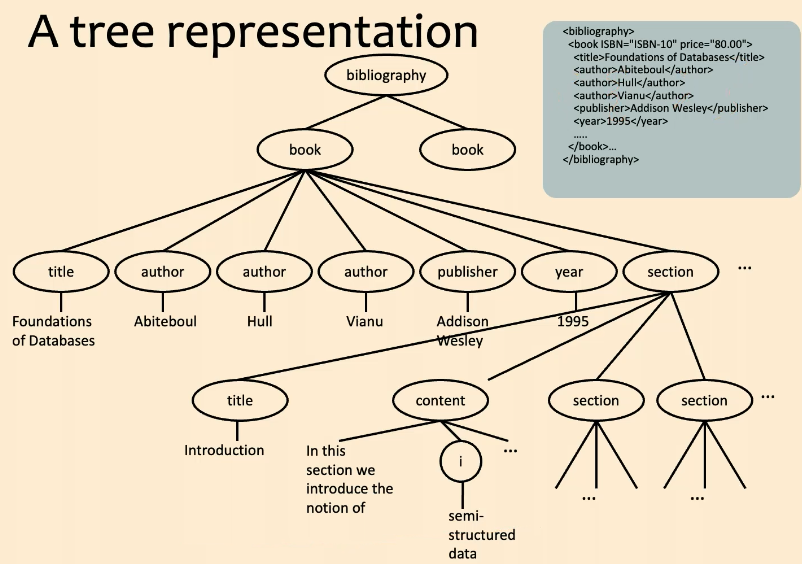
\includegraphics[scale=0.4]{img/tree_rep.png}
      \caption{Tree representation of an XML file.} 
      \label{fig:tree_rep}
    \end{figure}
  \end{example}

  Let's do a quick comparison of relations and XML. 
  \begin{enumerate}
    \item One advantage of XML is portability/exchangeability, since it self-describes itself, so all you really need is this text, unlike relations where you should also send the schema and other metadata. On the other hand, exchanging is problematic. 
    \item Second, its has flexibility to represent any information (e.g. structured, semi-structured, documents, etc.). Unlike a relation where each attribute of each tuple is atomic (meaning you can't place another relation in there), you can make a new XML tree. 
    \item Finally, since the data describes itself, you can change the schema easily. In contrast, the schema of a relational database is always fixed in advance and difficult to change. 
    \item Almost all major DBMS supports relations, and XML is often implemented as an add-on on top of relations. 
    \item Unlike the relational database where the order of the rows don't matter, the order does matter for XML. 
  \end{enumerate}
  
  \begin{definition}{DTD}
    Just because we don't need metadata does not mean that we cannot define one. This is done with the \textbf{document type definitions (DTD)}, which species the schema and constraints for XML just like relational databases. It has the following syntax, which should be written in the beginning of the XML file. 
    \begin{lstlisting}
      <!DOCTYPE root-element [
         <!ELEMENT element-name (content-specification)>
      ]> 
    \end{lstlisting} 
    Here are the common element specifications. 
    \begin{enumerate}
      \item \texttt{EMPTY}: Element has no content
      \item \texttt{ANY}: Element can contain any content
      \item \texttt{(\#PCDATA)}: Element contains parsed character data
      \item \texttt{Child elements}: Listed in parentheses
    \end{enumerate}
    with an example of a simple DTD being 
    \begin{lstlisting}
      <!DOCTYPE library [
         <!ELEMENT library (book+)>
         <!ELEMENT book (title, author, year)>
         <!ELEMENT title (#PCDATA)>
         <!ELEMENT author (#PCDATA)>
         <!ELEMENT year (#PCDATA)>
      ]> 
    \end{lstlisting}
  \end{definition}

  Really, this is like a tree directory structure, so to query data, it makes sense to try and traverse the paths. There are three major query languages for XML, which are 
  \begin{enumerate}
    \item \textbf{XPath}, which uses path expressions with conditions and are the building blocks of the rest of the standards. 
    \item \textbf{XQuery}, which is XPath plus a full-fledged SQL-like query language. 
    \item \textbf{XSLT}, or eXtensible Stylesheet Language Transformations and is the recommended style sheet language for XML. 
  \end{enumerate}

  \subsection{XPath}

    \begin{definition}[Basic XPath Constructs]
      The syntax for building a XPath is as follows: 
      \begin{enumerate}
        \item \texttt{/}: used as a separator between steps in a path (traversing down). 
        \item \texttt{name}: matches any child element with this tag name. 
        \item \texttt{*}: matches any child element 
        \item \texttt{\@name}: matches the attribute with this name. 
        \item \texttt{\@*}: matches any attribute 
        \item \texttt{//}: matches any descendent element of the current element itself. 
        \item \texttt{. }: matches current element.
        \item \texttt{. }: matches parent element.\footnote{This is just like when we are navigating directories in a shell.}
      \end{enumerate}
      Note that these names are all case sensitive, and another important fact is that NULL evaluates to NOT (so if there are no elements/attributes), then a condition on that element/attribute will evaluate to NOT. 
    \end{definition}

    \begin{example}
      Let's look at this example, which shows bibliographies for different books. 
      \begin{lstlisting}
        <?xml version="1.0" encoding="UTF-8"?>
        <bibliography>
            <book ISBN="ISBN-10" price="70">
                <title>Foundations of Databases</title>
                <author>Abiteboul</author>
                <author>Hull</author>
                <author>Vianu</author>
                <publisher>Addison Wesley</publisher>
                <year>1995</year>
                <section>abc</section>
            </book>
            <book ISBN="ISBN-11" price="20">
                <title>DBSTS</title>
                <author>Ramakrishnan</author>
                <author>Gehrke</author>
                <publisher>Addison Wesley</publisher>
                <year>1999</year>
                <section>
                  <title>bruh</title>
                </section>
            </book>
            <report>
              <author>Muchang</author>
              <addon>
                <author>Jon</author>
              </addon>
            </report>
        </bibliography> 
      \end{lstlisting}
      Let's look at some XPaths. 
      \begin{enumerate}
        \item \texttt{/bibliography/book/author} gets all author element reachable via this path.
          \begin{lstlisting}
            <author>Abiteboul</author>
            <author>Hull</author>
            <author>Vianu</author>
            <author>Ramakrishnan</author>
            <author>Gehrke</author>
          \end{lstlisting}

        \item \texttt{/bibliography/book/title} gets all book titles reachable via this path. 
          \begin{lstlisting}
            <title>Foundations of Databases</title>
            <title>DBSTS</title>
          \end{lstlisting}

        \item \texttt{/bibliography/book/\@ISBN} gets all book ISBN attributes (we need the \texttt{\@} to search the \textit{attribute}, not the element)
          \begin{lstlisting}
            ISBN="70"
            ISBN="ISBN:11"
          \end{lstlisting}

        \item \texttt{//title} returns all title elements, anywhere in the document. Note that the title of the section is also added. 
          \begin{lstlisting}
            <title>Foundations of Databases</title>
            <title>DBSTS</title>
            <title>bruh</title>
          \end{lstlisting}

        \item \texttt{//section/title} returns all section titles, anywhere in the document.
          \begin{lstlisting}
            <title>bruh</title>
          \end{lstlisting}

        \item \texttt{/bibliography/*/author} returns all authors in bibliography that is a grandchild of bibliography. Note that Muchang is retrieved but not Jon. 
          \begin{lstlisting}
            <author>Abiteboul</author>
            <author>Hull</author>
            <author>Vianu</author>
            <author>Ramakrishnan</author>
            <author>Gehrke</author>
            <author>Muchang</author>
          \end{lstlisting}

        \item \texttt{/bibliography/book[@price<50]} returns all books that are children of bibliography with attribute price less than 50. 
          \begin{lstlisting}
            <book ISBN="ISBN-11" price="20">
                <title>DBSTS</title>
                <author>Ramakrishnan</author>
                <author>Gehrke</author>
                <publisher>Addison Wesley</publisher>
                <year>1999</year>
                <section>
                  <title>bruh</title>
                </section>
            </book>
          \end{lstlisting}

        \item \texttt{/bibliography/book[author='Abiteboul']} returns all books that are children of bibliography that has an author tag children with element Abiteboul. 

        \item \texttt{/bibliography/book[author]} returns all books that are children of bibliography with some child author tag. 

        \item \texttt{\bibliography/book[40 <= @price and @price <= 50]} returns books with price attribute between 40 and 50. 

        \item \texttt{/bibliography/book[author='Abiteboul' or @price >=50]} returns books either authored by Abiteboul or price at least 50. Note that the first condition is on an element and the second is on an attribute. 

        \item \texttt{/bibliography/book[author='Abiteboul' or not (@price < 50)]} returns books authored by Abiteboul or price not below 50. Note that this is different from the query above since if a book does not have a price, then \texttt{\@price < 50} is null (which is NOT in XPath), so it returns the book. 
      \end{enumerate}
    \end{example}

    Hopefully you get a good feel for how XPaths work. Here's a trickier example. 

    \begin{example}[Conditions on Any vs All Attributes/Elements]
      Say you want to get all books with some price in the range $[20, 50]$. Then you would think of writing 
      \begin{lstlisting}
        /bibliography/book/[price>=20 and price <=50]
      \end{lstlisting}
      This may not work if we have a XML element of this form, with multiple prices. 
      \begin{lstlisting}
        <book> 
          <title>newbooktitle</title>
          <price>10</price>
          <price>70</price> 
        </book>
      \end{lstlisting} 
      since it compares is any element satisfies the conditions. Therefore, we can think of these conditions all as the \texttt{any} condition over child elements. If we want to use the \texttt{all} condition, we can write 
      \begin{lstlisting}
        /bibliography/book/[price[.>=20 and .<=50]]
      \end{lstlisting}

      Similarly, if we have the query \texttt{/bibliography/book[author='A' and author!='A']}, this is an any clause, so it will return all books with author A and another author not A. 
    \end{example}

    \begin{definition}[XPath Operators and Functions] 
      In conditions, we can use the following operations. 
      \begin{enumerate}
        \item Arithmetic: \texttt{x + y}, \texttt{x - y}, \texttt{x * y}, \texttt{x div y}, \texttt{x mod y} 
        \item \texttt{contains(x, y)} returns true if string \texttt{x} contains string \texttt{y} 
        \item \texttt{count(node-set)} counts the number of nodes in \texttt{node-set} 
        \item \texttt{position()} returns the \textit{context position} (i.e the position of the node amongst its siblings) 
        \item \texttt{last()} returns the \textit{context size} (roughly the size of the node-set)
        \item \texttt{name()} returns the tag name of the current element
      \end{enumerate}
    \end{definition}

    \begin{example}
      Some more queries is 
      \begin{enumerate}
        \item \texttt{/bibliography/book[count(section)<10]} returns books with fewer than 10 sections. 
        \item \texttt{//*[contains(name(), 'Ab')]} returns all elements whose tag names contain \texttt{Ab} (or \texttt{section}?) 
        \item \texttt{/bibliography/book/section[position()=1]/title} returns the title of the first section in each book. 
        \item \texttt{/bibliography/book/section[position()=last()]/title} returns the title of the last section in each book.
      \end{enumerate}
    \end{example}

  \subsection{XQuery}
    
    XQuery is a superset of the XPath, but it also encompasses FLWOR  expressions, quantified expressions, aggregation, sorting, etc. An XQuery expression can even return a new result XML document. Let's put the XML example file again for convenience. 

    \begin{lstlisting}
      <?xml version="1.0" encoding="UTF-8"?>
      <bibliography>
          <book ISBN="ISBN-10" price="70">
              <title>Foundations of Databases</title>
              <author>Abiteboul</author>
              <author>Hull</author>
              <author>Vianu</author>
              <publisher>Addison Wesley</publisher>
              <year>1995</year>
              <section>abc</section>
          </book>
          <book ISBN="ISBN-11" price="20">
              <title>DBSTS</title>
              <author>Ramakrishnan</author>
              <author>Gehrke</author>
              <publisher>Addison Wesley</publisher>
              <year>1999</year>
              <section>
                <title>bruh</title>
              </section>
          </book>
      </bibliography> 
    \end{lstlisting}

    \begin{example}
      For now, let's start with a simple XQuery based on XPath. To find all books, we can write the following, where the first \texttt{doc} refers to the specific document to query.
      \begin{lstlisting}
        <result>{
          doc("bib.xml")/bibliography/book
        }</result>
      \end{lstlisting}
      Note that like Python string interpolation, text outside of \texttt{\{\}} are copied to output verbatim, while those inside are evaluated and replaced by the result. We can use conditionals the same way. 
      \begin{lstlisting}
        <result>{
          doc("bib.xml")/bibliography/book[@price<50]
        }</result>
      \end{lstlisting}
      which will return 
      \begin{lstlisting}
        <book ISBN="ISBN-11" price="20">
            <title>DBSTS</title>
            <author>Ramakrishnan</author>
            <author>Gehrke</author>
            <publisher>Addison Wesley</publisher>
            <year>1999</year>
            <section>
              <title>bruh</title>
            </section>
        </book>
      \end{lstlisting}
    \end{example}

    \begin{definition}[FLWOR Expressions]
      The fundamental building block of XQuery is the FLWOR expression, which stands for:
      \begin{enumerate}
        \item \texttt{FOR}: Iterates over sequences
        \item \texttt{LET}: Binds variables to values
        \item \texttt{WHERE}: Filters the tuples
        \item \texttt{ORDER BY}: Sorts the results
        \item \texttt{RETURN}: Constructs the result
      \end{enumerate}
      Note that only the \texttt{RETURN} clause is mandatory; all others are optional.
    \end{definition}

    \begin{example}[FLWOR with Loops and Conditionals]
      To retreive the titles of books published before 2000, together with their publisher, we can write either of the following. The logic is pretty self explanatory. 

      \noindent\begin{minipage}{.5\textwidth}
      \begin{lstlisting}[]{Code}
        <result>{
          for $b in /bibliography/book 
          let $p := $b/publisher 
          where $b/year < 2000 
          return 
            <book>
            { $b/title }
            { $p }
            </book>
        }</result>
      \end{lstlisting}
      \end{minipage}
      \hfill
      \begin{minipage}{.49\textwidth}
      \begin{lstlisting}[]{Output}
        <result>{
          for $b in /bibliography/book[year<2000]
          return 
            <book>
            { $b/title }
            { $p/publisher }
            </book>
        }</result>
        .
        .
      \end{lstlisting}
      \end{minipage}
      which will return 
      \begin{lstlisting}
        <result>
          <book>
            <title>Foundations of Databases</title>
            <publisher>Addison Wesley</publisher>
          </book>
          <book>
            <title>DBSTS</title>
            <publisher>Addison Wesley</publisher>
          </book>
        </result> 
      \end{lstlisting}
      Note that \texttt{\$p} may be assigned to a set of elements. It does not have to be one element. 
    \end{example}

    Just like XPath, a conditional expression (with where) only checks the \texttt{any} condition. 
    
    \begin{example}[Nested Loops and List Comprehension]
      We can also use nested loops to solve the query above, but note the logic. If a book of price < 2000 has 2 publishers, then the book may be returned 2 times. On the other hand, if a book has a price < 2000 but has no publishers, then a null is really a false, so that book will not be returned. 

      \noindent\begin{minipage}{.5\textwidth}
        \begin{lstlisting}[]{Code}
          <result>
          {
            for $b in /bibliography/book,
            $p in $b/publisher
            where $b/year < 2000
            return 
              <book>{ $b/title }{ $p }</book>
          }
          </result> 
          .
          .
          .
          .
          .
        \end{lstlisting}
        \end{minipage}
        \hfill
        \begin{minipage}{.49\textwidth}
        \begin{lstlisting}[]{Output}
          <result>
            <book>
              <title>Foundations of Databases</title>
              <publisher>Addison Wesley</publisher>
            </book>
            <book>
              <title>Foundations of Databases</title>
              <publisher>Springer</publisher>
            </book>
            <book>
              <title>DBSTS</title>
              <publisher>Addison Wesley</publisher>
            </book>
          </result>          
        \end{lstlisting}
      \end{minipage}

      If we use a comprehension statement, we can let \texttt{\$b} be all the books and try to parse them element by element where its year is < 2000. This is also wrong since the where clause is an any expression, so if at least 2 book has year < 2000, then it will return all the books. In fact, it doesn't even return it in the right format, since it returns all the book titles first and then all the publishers. 

      \noindent\begin{minipage}{.5\textwidth}
        \begin{lstlisting}[]{Code}
          <result>
          {
            let $b := /bibliography/book
            where $b/year < 2000
            return 
              <book>
                { $b/title }
                { $b/publisher }
              </book>
          }
          </result>          
        \end{lstlisting}
        \end{minipage}
        \hfill
        \begin{minipage}{.49\textwidth}
        \begin{lstlisting}[]{Output}
          <result>
            <book>
              <title>Found of Databases</title>
              <title>DBSTS</title>
              <publisher>Addison Wesley</publisher>
            </book>
          </result>
          .
          .
          .
          .
        \end{lstlisting}
      \end{minipage}
    \end{example}

    Now that we went over FLWOR, let's talk about how we can do joins. 

    \begin{example}[Explicit Join]
      To find all pairs of books that have common authors, we can write 
      \begin{lstlisting}
        <result>
        {
          for $b1 in //book
          for $b2 in //book
          where $b1/author = $b2/author
          and $b1/title > $b2/title
          return
            <pair>
              { $b1/title }
              { $b2/title }
            </pair>
        }
        </result> 
      \end{lstlisting}
      Remember that since the where is an any condition, this works to our advantage now. We also use a string comparison of the authors and titles to remove duplicates. This gives us the result. 
      \begin{lstlisting}
        <result>
          <pair>
            <title>Foundations of Databases</title>
            <title>DBSTS</title>
          </pair>
        </result> 
      \end{lstlisting}
    \end{example}

    We will stop here, but there are more features such as subqueries, existential (some) vs universal (all) queries, aggregation, conditional, etc. 

  \subsection{Converstion of XML to Relational Data} 
    
    Relational to XML is trivial, but XML to relational isn't really since there can be different data types that are siblings (e.g. books vs articles, vs papers all under bibliography), there may be repeats of the same tag, and there are both child elements and attributes. 
    
    The most trivial thing to do is to store the entire XML in a column (called a CLOB, character large Object type), but this isn't useful since it first does not satisfy the condition that each element must be atomic in a relation. There are two alternatives. 
    \begin{enumerate}
      \item \textbf{Schema-Oblivious Mapping} takes a well-formed XML and converts it to a generic relational schema. In here, there are more subtypes. 
        \begin{enumerate}
          \item \textbf{Node/edge based mapping} for graphs. 
          \item \textbf{Interval based mapping} for trees.
          \item \textbf{Path based mapping} for trees. 
        \end{enumerate}
      \item \textbf{Schema-Aware Mapping} takes a valid XML and converts it to a special relational schema based on DTD. 
    \end{enumerate} 

    Let's go over the node/edge based mapping. This is quite intuitive since we can visualize a XML structure as a directed graph. 
    \begin{figure}[H]
      \centering 
      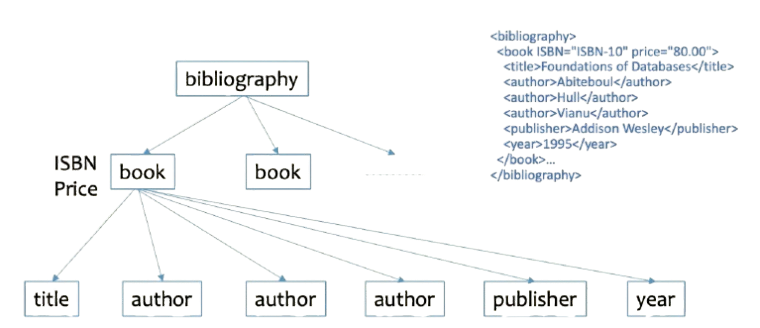
\includegraphics[scale=0.25]{img/node_based.png}
      \caption{} 
      \label{fig:node_based}
    \end{figure}

    We can convert the XML to the following 4 relations. We also put the bibliography example to make it easier to follow along. 
    \begin{enumerate}
      \item \textbf{Element(\underline{eid}, tag)}. All elements will have a certain id with their tag type. Note that elements can have text inside of them, but we will consider this a ``child'' of the element, stored in the \texttt{Text} relation. 

        \begin{table}[H]
          \centering
          \caption{Element Table}
          \begin{tabular}{|l|l|}
            \hline
            \textbf{eid} & \textbf{tag} \\
            \hline
            e0 & bibliography \\
            e1 & book \\
            e2 & title \\
            e3 & author \\
            e4 & author \\
            e5 & author \\
            e6 & publisher \\
            e7 & year \\
            \hline
          \end{tabular}
          \caption{}
          \label{tab:}
        \end{table}

      \item \textbf{Attribute(eid, attrName, attrValue)}. All attributes will need to have their name and type, along with which eid that they are a part of. Note that there is only one functional dependency \texttt{(eid, attrName) -> attrValue}.

        \begin{table}[H]
          \centering
          \caption{Attribute Table}
          \begin{tabular}{|l|l|l|}
          \hline
          \textbf{eid} & \textbf{attrName} & \textbf{attrValue} \\
          \hline
          e1 & ISBN & ISBN-10 \\
          e1 & price & 80 \\
          \hline
          \end{tabular}
        \end{table}

      \item \textbf{ElementChild(eid, pos, child)}. Each element will have a children, with pos referring to the position of the children. Child references either \texttt{Element(eid)} or \texttt{Text(tid)}. 

        \begin{table}[H]
          \centering
          \caption{ElementChild Table}
          \begin{tabular}{|l|l|l|}
          \hline
          \textbf{eid} & \textbf{pos} & \textbf{child} \\
          \hline
            e0 & 1 & e1 \\
            e1 & 1 & e2 \\
            e1 & 2 & e3 \\
            e1 & 3 & e4 \\
            e1 & 4 & e5 \\
            e1 & 5 & e6 \\
            e1 & 6 & e7 \\
            e2 & 1 & t0 \\
            e3 & 1 & t1 \\
            e4 & 1 & t2 \\
            e5 & 1 & t3 \\
            e6 & 1 & t4 \\
            e7 & 1 & t5 \\
          \hline
          \end{tabular}
        \end{table}

      \item \textbf{Text(\underline{tid}, value)}. All text in an element, with an id value (which cannot be the same as any eid) and the actual text in the value. 

        \begin{table}[H]
          \centering
          \caption{Text Table}
          \begin{tabular}{|l|l|}
          \hline
          \textbf{tid} & \textbf{value} \\
          \hline
          t0 & Foundations of Databases \\
          t1 & Abiteboul \\
          t2 & Hull \\
          t3 & Vianu \\
          t4 & Addison Wesley \\
          t5 & 1995 \\
          \hline
          \end{tabular}
        \end{table}
    \end{enumerate}
    Note that we need to invent a lot of ids and need indices for efficiency. 


    Given this, we can write the equivalent SQL queries from these XPath queries. 
    \begin{enumerate}
      \item \texttt{//title} 
        \begin{lstlisting}
          SELECT eid FROM Element WHERE tag='title';
        \end{lstlisting}

      \item \texttt{//section/title} 
        \begin{lstlisting}
          SELECT e2.eid 
          FROM Element e1, ElemtnChild c, Element e2 
          WHERE e1.tag = 'section' 
          AND e2.tag = 'title' 
          AND e1.eid = c.eid 
          AND c.child = e2.eid;
        \end{lstlisting}
        Therefore, path expression becomes joins. The number of joins is proportional to the length of the path expression. 
    \end{enumerate}

\section{Query Processing and Optimization} 
  
    When the DBMS chooses the best way to sort or merge two relations, it needs to choose it immediately. This can be done crudely by looking at the statistics of the relations that it is working with, but it doesn't guarantee that you will get the optimal plan. Therefore, it goes by the principal that you shouldn't try and waste time choosing the optimal one, but rather avoid the horrible ones. 

    As a user of this DBMS, we should also take care in writing queries that are not too computationally or IO heavy. Two general heuristics that we should follow are: 
    \begin{enumerate}
      \item You want to \textit{push down}, i.e. use as early as possible, selections and projections. 
      \item You want to join smaller relations first and avoid using cross product, which can be devastating in memory. 
    \end{enumerate}

    We can get a bit more theoretical and use the following identities in relational algebra. 

    \begin{theorem}[Identities]
      The following hold:
      \begin{enumerate}
        \item Selection-Join Conversion: $\sigma_p(R \times S) = R \bowtie_p S$
        \item Selection Merge/Split: $\sigma_{p_1}(\sigma_{p_2}R) = \sigma_{p_1 \wedge p_2}R$
        \item Projection Merge/Split: $\pi_{L_1}(\pi_{L_2}R) = \pi_{L_1}R$, where $L_1 \subseteq L_2$
        \item Selection Push Down/Pull Up: $\sigma_{p \wedge p_r \wedge p_s}(R \bowtie_{p'} S) = (\sigma_{p_r}R) \bowtie_{p \wedge p'} (\sigma_{p_s}S)$, where:
        - $p_r$ is a predicate involving only R columns
        - $p_s$ is a predicate involving only S columns
        - $p$ and $p'$ are predicates involving both R and S columns
        \item Projection Push Down: $\pi_L(\sigma_p R) = \pi_L(\sigma_p(\pi_{L L'}R))$, where:
        - $L'$ is the set of columns referenced by $p$ that are not in $L$
      \end{enumerate}
    \end{theorem} 

  \subsection{Rewriting SQL Queries}

    \begin{definition}[SQL Query Rewrite]
      We can rewrite SQL queries directly, though this is more complicated and requires knowledge of the nuances of the DBMS. 
      \begin{enumerate}
        \item Subqueries and views may not be efficient, as they divide a query into nested blocks. Processing each block separately forces the DBMS to use join methods, which may not be optimal for the entire query though it may be optimal for each block. 
        \item Unnest queries convert subqueries/views to joins. 
      \end{enumerate}
      Therefore, it is usually easier to deal with select-project-join queries, where the rules of relational algebra can be cleanly applied. 
    \end{definition} 

    \begin{example}[Query Rewrite]
      Given the query, we wish to rewrite it. 
      \begin{lstlisting}
        SELECT name 
        FROM User 
        WhERE uid = ANY(SELECT uid FROM Member);
      \end{lstlisting}

      The following is wrong since there may be one user in two groups, so it will be duplicated.\footnote{A bit of review: when testing whether two queries are equal, think about if the two queries treat duplicates, null values, and empty relations in the same way. } 
      \begin{lstlisting}
        SELECT name 
        FROM User, Member 
        WHERE User.uid = Member.uid;
      \end{lstlisting} 

      The following is correct assuming \texttt{User.uid} is a key. 
      \begin{lstlisting}
        SELECT name 
        FROM (SELECT DISTINCT User.uid, name) 
        FROM User, Member 
        WHERE User.uid = Member.uid); 
      \end{lstlisting}
    \end{example}

    \begin{example}[Correlated Subqueries]
      Look at this query where we want to select all group ids with name like Springfield and having less than some number of members. 
      \begin{lstlisting}
        SELECT gid 
        FROM Group, (SELECT gid, COUNT(*) AS cnt FROM Member GROUP BY gid) t 
        WHERE t.gid = Group.gid AND min_size > t.cnt 
        AND name LIKE 'Springfield%';
      \end{lstlisting}
      This is inefficient since for every \texttt{gid}, we are making an entire extra query to select the counts. This is called a \textbf{non-correlated} query since this subquery is being run independently for every run. It ends up computing the size of \textit{every} group, unlike the following one, where it filters out groups named Springfield first and then computes their size. 
      \begin{lstlisting}
        SELECT gid FROM Group 
        WHERE name LIKE 'Springfield%' 
        AND min_size > (SELECT COUNT(*) FROM Member WHERE Member.gid = Group.gid);
      \end{lstlisting}
    \end{example}
  
  \subsection{Logical and Physical Plans}

    We can construct a high-level \textbf{logical plan}, which shows the computation DAG of the relational operators that we will perform for a query. We can optimize the logical plan by modifying the intermediate steps with the following identities. They may or may not help in the runtime, since they are dependent on the size of the intermediate inputs. On the implementation side, we want to show the \textbf{physical plan}, which is the actual implementation including even more operations in between each node of the logical plan. This may include scanning or sorting. 

    The difference between the logical and physical plan is that the logical plan represents \textit{what} needs to be done and not \textit{how}. Consider the two approaches. 

    \begin{example}[Query Plans]
      Consider the following SQL query:
      \begin{lstlisting}
        SELECT Group.title
        FROM User
        JOIN Member ON User.uid = Member.uid
        JOIN Group ON Member.gid = Group.gid
        WHERE User.name = 'Bart';
      \end{lstlisting}

      \begin{figure}[H]
        \centering 
        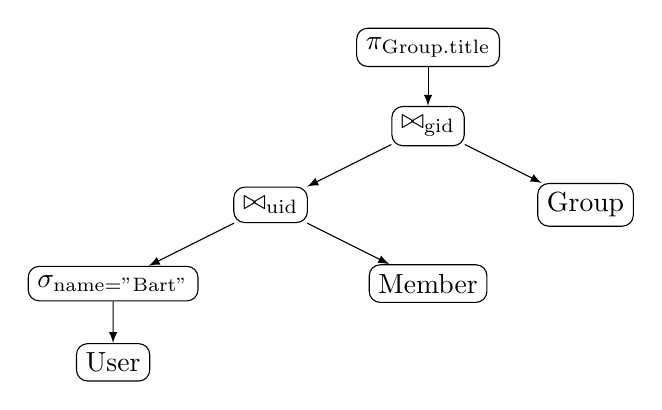
\begin{tikzpicture}[
            level distance=1.0cm,
            every node/.style={draw, rounded corners}, 
            sibling distance=4cm,
            edge from parent/.style={draw, -latex}
        ]
        \node {$\pi_{\text{Group.title}}$}
            child {
                node {$\bowtie_{\text{gid}}$}
                child {
                    node {$\bowtie_{\text{uid}}$}
                    child {
                        node {$\sigma_{\text{name="Bart"}}$}
                        child {
                            node {User}
                        }
                    }
                    child {
                        node {Member}
                    }
                }
                child {
                    node {Group}
                }
            };
        \end{tikzpicture}
        \caption{Logical Plan. We first take User, select Bart, and join it to Member over uid. Then we join it with Group on gid, and finally project the title attribute.} 
        \label{fig:logical_plan}
      \end{figure}

      \begin{figure}[H]
        \centering 
        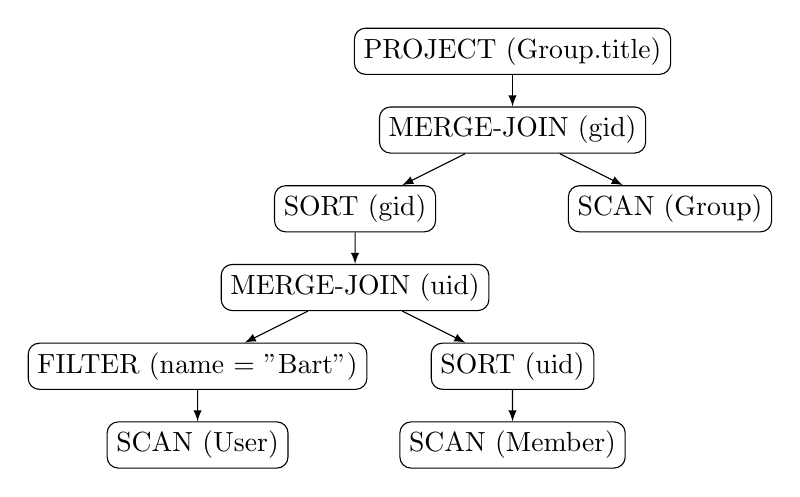
\begin{tikzpicture}[
            level distance=1.0cm,
            sibling distance=4cm,
            every node/.style={draw, rounded corners},
            edge from parent/.style={draw, -latex}
        ]
        \node {PROJECT (Group.title)}
            child {
                node {MERGE-JOIN (gid)}
                child {
                    node {SORT (gid)}
                    child {
                        node {MERGE-JOIN (uid)}
                        child {
                            node {FILTER (name = "Bart")}
                            child {
                                node {SCAN (User)}
                            }
                        }
                        child {
                            node {SORT (uid)}
                            child {
                                node {SCAN (Member)}
                            }
                        }
                    }
                }
                child {
                    node {SCAN (Group)}
                }
            };
        \end{tikzpicture}
        \caption{Physical Plan. We first take User and do a scan before filtering/selecting tuples with Bart. We also scan Member and sort it by uid in order to prepare for merge-join. Once we merge-join over uid, we sort it again to prepare a second merge-join with Group (which we scan first). Once we do this, we finally project the title attribute. } 
        \label{fig:physical_plan}
      \end{figure}
    \end{example} 

  \subsection{Cardinality Estimation}

    In the physical plan, we need to have a cost estimation for each operator. For example, we know that \texttt{SORT(gid)} takes $O(B(\text{input}) \cdot \log_M B(\text{input}))$, but we should find out what $B$, the number of blocks needed to store our input relation, is. To do this, we need the size of intermediate results through cardinality estimation.  

    Usually we cannot do quick and accurate cardinality estimation without strong assumptions, the first of which is uniformity of data. 

    \begin{example}[Selection with Equality Predicates]
      Suppose you have a relation $R$ with $|R| = 100,000$ tuples. Assume that it has an attribute $A$ taking integer values in $[50, 100)$ \textit{distributed uniformly}. Then, there are 50 distinct values, and when we want to do $\sigma_{A = a} (R)$, then we would expect it to return 
      \begin{equation}
        |\sigma_{A = a} (R)| = \frac{|R|}{|\pi_A(R)|} = 2000
      \end{equation}
      tuples.
    \end{example}

    The second assumption is \textit{independence} of the distributions over each attribute. 

    \begin{example}[Selection with Conjunctive Predicates]
      If we have the same relation $R$ with integer attributes $A \in [50, 100), B \in [10, 20)$ independently and uniformly distributed. Then, 
      \begin{equation}
        |\sigma_{A = a, B = b} (R) = \frac{|R|}{|\pi_A (R)| \cdot |\pi_B(R)|} = \frac{100,000}{50 \cdot 10} = 200
      \end{equation}
    \end{example}

    At this point, we are just using inclusion-exclusion principle and this becomes a counting problem. 

    \begin{example}[Negated, Disjunctive Predicates]
      We list these identities for brevity. The math is pretty simple. 
      \begin{equation}
        |\sigma_{A \neq a} (R)| = |R| \cdot \bigg( 1 - \frac{1}{|\pi_A (R)|} \bigg)
      \end{equation}
      and using I/E principle, we have 
      \begin{equation}
        |\sigma_{A = a \lor B = b} (R)| = |R| \cdot \bigg( \frac{1}{|\pi_A (R)|}  + \frac{1}{|\pi_B (R)|} - \frac{1}{|\pi_A (R)| \cdot |\pi_B(R)|} \bigg)
      \end{equation}
    \end{example}

    \begin{example}[Range Predicates]
      Range also works similarly, but only if we know the actual bounds of the attribute values.  
      \begin{equation}
        |\sigma_{A > a} (R)| = |R| \cdot \frac{\max(R.A) - a}{\max(R.A) - \min(R.A)}
      \end{equation}
    \end{example}

    Clearly, if we know that an attribute follows, say a Gaussian or a Poisson distribution, we can just calculate the difference in the CDFs and scale up by the relation size to get the approximate cardinality. I think this is what the professor refers to as \textit{histogram estimation}. 

    For joins, we need yet another assumption, called \textit{containment of value sets}. This means that if we are natural joining $R(A, B) \bowtie S(A, C)$, every tuple in the smaller (as in fewer distinct values for the join attribute $A$) joins with some tuple in the other relation. In other words, 
    \begin{equation}
      |\pi_A (R)| \leq |\pi_A (S)| \implies \pi_A (R) \subset \pi_A (S)
    \end{equation}
    which again is a very strong assumption in general but holds in the case of foreign key joins. 

    \begin{example}[Two Way Equi-Join] 
      With the containment assumption, we have 
      \begin{equation}
        |R \bowtie_{A} S| = \frac{|R| \cdot |S|}{\max( |\pi_A (R)|, |\pi_A(S)|)}
      \end{equation} 
      Think of this as looking at the cross product between the two relations, and then filtering out the actual tuples that don't belong there.  
    \end{example}

  \subsection{Search Strategies} 

    Say that we have relations $R_1, \ldots, R_n$ that we want to join. The set of all sequences in which we can join them is bijective to the set of all binary trees with leaves $R_i$. This grows super-exponentially, reading $30,240$ for $n = 6$. There are too many logical plans to choose from, so we must reduce this search space. Here are some heuristics. 
    \begin{enumerate}
      \item We consider only \textbf{left-deep} plans, in which case every time we join two relations, it is the outer relation in the next join.\footnote{Note that since the right/inner relation is the one that is being scanned, we want the right one to be smaller since for each block of the left relation, we are looping over all blocks of the right relation. Therefore, left-deep plans are much more efficient since we don't have to scan the huge relation from the disk multiple times. We can just send it directly to the next join.} 

      \begin{figure}[H]
        \centering 
        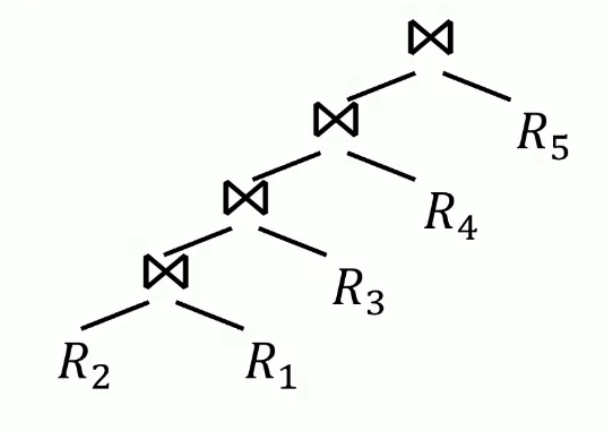
\includegraphics[scale=0.4]{img/left_deep.png}
        \caption{Left deep plans have a search space of only $n!$, which is better than before. } 
        \label{fig:left_deep}
      \end{figure} 

      \item We can consider a balance binary tree, which can be parallel processed, but this causes more runtime on the CPU in sort-merge joins, you must materialize the result in the disk, and finally the search space of binary trees may be larger than that of the left-deep tree. 
    \end{enumerate}

    Even left-deep plans are still pretty bad, and so optimizing this requires a bit of DP (dynamic programming), using \textit{Selinger's algorithm}. Given $R_1, \ldots, R_n$, we must choose a permutation from the $n!$ permutations. Say that the cost of the optimal join of a set $\mathbb{R}$ is $f(\mathbb{R})$. Note the recursive formula for some $S \subset [n]$. 
    \begin{equation}
      f(\{R_i\}_{i \in S}) = \min_i f(\{R_j\}_{j \in S, j \neq i}) + f(R_i, \bowtie_{j \in S, j \neq i} R_j) 
    \end{equation}
    Where we sum up the cost of getting the accumulated relation and add it to the additional cost of joining once more with $R_i$. Therefore, given the $R_i$'s, 
    \begin{enumerate}
      \item We compute all $f(\{R_i, R_j\})$ for $i < j$ (since $j > i$ requires us the larger one to be inner). 
      \item Then we apply the recursive formula for all 3-combinations and so on, until we get to $n$-combinations. 
    \end{enumerate}

\section{JSON}

  NoSQL just stands for not SQL or not relational, like XML or \textbf{JSON}.\footnote{I think it's called this because it's literally how JS objects are stored and printed.} This relaxes some constraints and may be more flexible/efficient, with some popular data stores being MongoDB, CouchDB, Dynamo, etc. They are designed to scale simple OLTP (online transaction processing) style application loads and provide good horizontal scalability. An example of where this is used is in pretty much all blockchains. Every transaction and block is accessible in a JSON format on say \texttt{etherscan.io}. 

  \begin{definition}[JSON]
    A \textbf{JSON}, short for \textbf{JavaScript Object Notation}, data model is an object with the following properties: 
    \begin{enumerate} 
      \item At the top level, it is an array of \textit{objects}. 
      \item Each object contains a set of key-value pairs of form \texttt{\{key : value\}}, where key (attribute) names should be unique within an object. 
      \item It supports most primitive types (numbers, strings, double, booleans are stored in quotes e.g. \texttt{"true"}), along with arrays \texttt{[...]}, and finally \textbf{objects} \texttt{\{...\}} (which defines a recursive structure). 
      \item The order is unimportant. 
      \item You can't comment in JSON files. 
    \end{enumerate}
  \end{definition}

  \begin{example}[Example JSON]
    Here is an example with users, groups, and members. 
    \begin{lstlisting}
      {
        "users": [
          {"uid": 1, "name": "Bart"},
          {"uid": 2, "name": "Lisa"}
        ],
        "groups": [
          {"gid": 101, "title": "Skateboarding Club"},
          {"gid": 102, "title": "Chess Club"}
        ],
        "members": [
          {"uid": 1, "gid": 101},
          {"uid": 1, "gid": 102},
          {"uid": 2, "gid": 102}
        ]
      } 
    \end{lstlisting}
  \end{example}

  \begin{definition}[MongoDB Database]
    A database has collections of similarly structured documents, similar to tables of records as opposed to one big XML document that contains all data.  
    \begin{enumerate}
      \item \textbf{Database} is a list of collections. (analogous to a database)
      \item \textbf{Collection} is a list a documents (analogous to a table)
      \item \textbf{Document} is a JSON object (analogous to a row/tuple)
    \end{enumerate}
    MongoDB actually stores this data with \textbf{BSON} (Binary JSON), which is the binary encoding of it. 
  \end{definition}  

  MongoDB provides a rich set of operations for querying and manipulating data. 

  \begin{definition}[find()]
    The \texttt{find()} operation is MongoDB's basic query mechanism. It returns a cursor to the matching documents.
    \begin{enumerate}
      \item Takes a query document that specifies the selection criteria
      \item Can include projection to specify which fields to return
      \item Supports comparison operators like \texttt{\$eq}, \texttt{\$gt}, \texttt{\$lt}
      \item Can query nested documents and arrays
    \end{enumerate}
  \end{definition}

  \begin{example}[Basic Query]
    Find all users named "Bart":
    \begin{lstlisting}
      db.users.find({"name": "Bart"})
    \end{lstlisting}
    Find users with uid greater than 1:
    \begin{lstlisting}
      db.users.find({"uid": {$gt: 1}})
    \end{lstlisting}
  \end{example}

  \begin{definition}[sort()]
    The \texttt{sort()} method orders the documents in the result set.
    \begin{enumerate}
      \item Takes a document specifying the fields to sort by
      \item Use 1 for ascending order, -1 for descending
      \item Can sort by multiple fields
      \item Applied after the query but before limiting results
    \end{enumerate}
  \end{definition}

  \begin{example}[Sorting]
    Sort users by name in ascending order:
    \begin{lstlisting}
      db.users.find().sort({"name": 1})
    \end{lstlisting}
  \end{example}


  \begin{definition}[Aggregation Pipeline]
    An aggregation pipeline consists of stages that transform sequences of documents. Each stage performs an operation on the input documents and passes the results to the next stage. Despite its name, it handles more than just aggregation operations.
  \end{definition}

  MongoDB supports several types of pipeline stages:

  \begin{enumerate}
    \item \textbf{Selection and Filtering} (\texttt{\$match})
    \begin{itemize}
        \item Filters documents based on specified conditions
        \item Similar to \texttt{find()} but within the pipeline context
    \end{itemize}

    \item \textbf{Projection} (\texttt{\$project})
    \begin{itemize}
        \item Reshapes documents by including, excluding, or transforming fields
        \item Can create computed fields
    \end{itemize}

    \item \textbf{Sorting} (\texttt{\$sort})
    \begin{itemize}
        \item Orders documents based on specified fields
        \item Equivalent to the \texttt{sort()} method
    \end{itemize}

    \item \textbf{Grouping} (\texttt{\$group})
    \begin{itemize}
        \item Groups documents by a specified expression
        \item Supports aggregation operators:
            \begin{itemize}
                \item \texttt{\$sum}: Calculates numeric totals
                \item \texttt{\$push}: Accumulates values into an array
            \end{itemize}
    \end{itemize}

    \item \textbf{Document Transformation}
    \begin{itemize}
        \item \texttt{\$project}/\texttt{\$addFields}: Adds computed fields
        \item \texttt{\$unwind}: Deconstructs arrays into individual documents
        \item \texttt{\$replaceRoot}: Promotes an embedded document to the top level
        \item Array operators:
            \begin{itemize}
                \item \texttt{\$map}: Applies an expression to each array element
                \item \texttt{\$filter}: Selects array elements matching a condition
            \end{itemize}
    \end{itemize}

    \item \textbf{Joining} (\texttt{\$lookup})
    \begin{itemize}
        \item Performs left outer joins with other collections
    \end{itemize}
  \end{enumerate}

  \begin{example}[Basic Pipeline]
    A pipeline that finds users in the "Chess Club" and sorts them by name:
    \begin{lstlisting}
      db.members.aggregate([
          {$lookup: {
              from: "users",
              localField: "uid",
              foreignField: "uid",
              as: "user"
          }},
          {$match: {"gid": 102}},
          {$sort: {"user.name": 1}}
      ])
    \end{lstlisting}
  \end{example}

  \begin{example}[Complex Pipeline]
    A pipeline using multiple stages to group and transform data:
    \begin{lstlisting}
      db.members.aggregate([
          {$group: {
              _id: "$gid",
              members: {$push: "$uid"},
              count: {$sum: 1}
          }},
          {$lookup: {
              from: "groups",
              localField: "_id",
              foreignField: "gid",
              as: "group_info"
          }},
          {$project: {
              _id: 0,
              group: {$arrayElemAt: ["$group_info.title", 0]},
              member_count: "$count",
              members: 1
          }}
      ])
    \end{lstlisting}
  \end{example}
  
  The pipeline stages must be carefully ordered as each stage's output becomes the input for the next stage. For optimal performance:
  \begin{enumerate}
    \item Use \texttt{\$match} early to reduce the number of documents
    \item Place \texttt{\$project} and \texttt{\$unwind} before \texttt{\$group} when possible
    \item Consider memory limitations when using \texttt{\$sort}
  \end{enumerate}

  \begin{definition}[\$lookup]
    The \texttt{\$lookup} operation performs a left outer join to another collection.
    \begin{enumerate}
      \item Must be used within an aggregation pipeline
      \item Specifies foreign collection to join with
      \item Defines local and foreign fields to join on
      \item Results stored in an array field
    \end{enumerate}
  \end{definition}

  \begin{example}[Join Operation]
    Join members with users:
    \begin{lstlisting}
      db.members.aggregate([
        {$lookup: {
          from: "users",
          localField: "uid",
          foreignField: "uid",
          as: "user_info"
        }}
      ])
    \end{lstlisting}
  \end{example}

  \begin{definition}[Aggregation Operators]
    Special operators used within aggregation pipelines for computations.
    \begin{enumerate}
      \item \texttt{\$sum}: Calculates sum of numeric values
      \item \texttt{\$push}: Adds value to an array
      \item \texttt{\$avg}: Calculates average
      \item \texttt{\$first}/\texttt{\$last}: Returns first/last value in group
    \end{enumerate}
  \end{definition}

  \begin{example}[Aggregation Operators]
    Calculate total members and collect group IDs:
    \begin{lstlisting}
      db.members.aggregate([
        {$group: {
          _id: "$uid",
          total: {$sum: 1},
          groups: {$push: "$gid"}
        }}
      ])
    \end{lstlisting}
  \end{example}

\section{Transactions} 

    So far, we've had one query/update on one machine, but this is not the case in reality. In modern systems, you have users interacting with a database all the time and databases may be prone to failure. These two situations requires us to develop a safer way of interacting with the database. 

    \begin{example}[Simultaneous Interaction]
      In an airline, say that we have two parties A and B trying to book the same seat. A looks at the website, which queries the tuple representing the seat. B does the same. A and B then both book it at the same time, sending an update request to the database, causing an overbooking. 

      In a bank, say that we have some events that must be recorded in a database. Say that $A = 0$ and $B = 100$. 
      \begin{enumerate}
        \item T1. B sends \$100 to A. So $A \mapsto A + 100, B \mapsto B - 100$. 
        \item T2. The bank sends all users an interest of 6\%. $A \mapsto 1.06 A, B \mapsto 1.06B$. 
      \end{enumerate}
      This is sensitive to order and perhaps at the end we expect $A = 100$. Consider the following cases. 
      \begin{enumerate} 
        \item $A \mapsto A + 100, B \mapsto B - 100, A \mapsto 1.06A, B \mapsto 1.06B$. This is fine. 
        \item $A \mapsto A + 100, A \mapsto 1.06A, B \mapsto 1.06B, B \mapsto B - 100$. This is not fine since both A and B got interest and the bank lost \$6. 
      \end{enumerate}
    \end{example}

    \begin{example}[Database Crash]
      If $A \mapsto A + 100$ happened first and the bank crashed, then the system would find that $A$ just gained \$100! This is clearly not good, so we must undo what we have done so far. 
    \end{example}

    These two examples hint at some nice properties that we want in our database. 
    \begin{enumerate}
      \item \textit{Serializability}. The first example shows that we do not like parallelism and rather we want things to run \textit{serially} in a way such that T1 and T2 occur separately, like a mutex lock. In practice, there are so many requests that parallelism is a must, so we must find ways to not run serially, but to modify our parallel computing to make it serializable, as if it is running serially.  
      \item \textit{Atomicity}. The second example shows that we want these operations to be \textit{atomic}, i.e. it is fully done or not done at all. That is, we do not want to update the disk (which preserves its state upon powering off) until  T1 is completely finished. A simple solution is to do all the operations in memory (which is wiped upon crashing anyways) and then \textit{commit} (announce that it is done) these changes. \footnote{Committing is not the same as disk writing, actually. It is not necessarily the case that one follows the other, so you can commit before writing and write before committing. There can also be some completed transactions with updated data still in memory and therefore lost in crash.} 
    \end{enumerate} 

    \begin{definition}[Transaction]
      The solution to both serializability and atomicity is to use \textbf{transactions}, which is a collection of one or more operations, called \textbf{actions}, on the database that must be executed atomically as a whole. At the end of every transaction, the DBMS always puts either a commit (indicating successful completion) or abort signal. 
    \end{definition} 

    \begin{definition}[ACID]
      These properties are a subset of the \textbf{ACID} properties.
      \begin{enumerate}
        \item \textit{Atomicity}. A user can think of a transaction as always executing all actions in one stop or not executing any at all. In an abort, this can be undone by storing recovery logs and going through the history to undo. 
        \item \textit{Consistency}. Each transaction, when run by itself with no concurrent execution of other actions, must preserve the consistency of the database.\footnote{e.g. if you transfer money from one account to another, the total amount in circulation still remains the same. The constraints must also be maintained. } 
        \item \textit{Isolation}. A user should be able to understand a transaction without considering the effect of any other concurrently running transaction. This allows us to have \textit{concurrency control}, which handles multiple transactions by interweaving them in a serializable way (like the bank example we saw above), and sometimes they may ensure isolation with locks.  

        \item \textit{Durability}. Once the DBMS informs the user that a transaction is completed, its effect should persist.\footnote{Even if the system crashes before writing to disk, we can recover it by using the history logs and redoing them.}
      \end{enumerate}
    \end{definition}

    \begin{definition}[Schedule]
      Now that we've cleared up on transactions, a schedule is simply a sequence of actions gotten from interweaving the transactions on the DBMS. It must obviously be consistent, and two actions from the same transaction T must appear in the schedule in the same order that they appear in T. Some examples of actions that can occur in a schedule is: 
      \begin{enumerate}
        \item \texttt{READ} 
        \item \texttt{WRITE}
        \item \texttt{COMMIT}
        \item \texttt{ABORT} 
      \end{enumerate}
      Some terminology to compare schedules: 
      \begin{enumerate}
        \item \textbf{Serial Schedule}. No interweaving of transactions. 
        \item \textbf{Equivalent Schedule}. Two schedules that have the same effect on the database state after completion. 
        \item \textbf{Serializable Schedule}. A schedule that is equivalent to a serial schedule. 
      \end{enumerate}
    \end{definition}

    \begin{example}[Bank Schedule]
      For the bank example above, we can construct a serial schedule $S_1$. 
      \begin{lstlisting}
        T1: R(A) W(A) R(B) W(B) C(T1)
        T2:                           R(A) W(A) R(B) W(B) C(T2)
      \end{lstlisting}
      and a serializable schedule $S_2$. 
      \begin{lstlisting}
        T1: R(A) W(A)                           R(B) W(B) C(T1)
        T2:           R(A) W(A) R(B) W(B) C(T2)
      \end{lstlisting}
      We can verify that $S_1 \equiv S_2$. 
    \end{example} 


  \subsection{Isolation Levels}

    When we interweave actions, conflicts may arise if one transaction wants to write to a data that another transactions reads/writes. This causes schedules that are not equivalent to the serial schedule. 
    \begin{enumerate}
      \item Write-Read (WR): reading uncommited or \textit{dirty data} 
      \item Read-Write (RW): unrepeatable reads. 
      \item Write-Write (WW): overwriting uncommitted data or lost updates, which can happen in the same or different transactions. 
      \item RR has no conflicts since there are no writes. 
    \end{enumerate}

    In SQL a transaction is automatically started when a user executes a SQL statement, and subsequent statements in the same session are executed as part of this transaction. Statements see changes made by earlier ones in the same transaction and statements in other concurrently running transactions do not. \texttt{COMMIT} and \texttt{ROLLBACK} commands are self explanatory.  
     
    SQL also supports isolation levels, which increases performance by eliminating overhead and allowing higher levels of concurrency, albeit at the cost of getting inconsistent answers if you don't know what you're doing. We start off with the most restrictive and go down. 
    \begin{enumerate}
      \item \texttt{SERIALIZABLE} is the strongest isolation level, with complete isolation. 

      \item \texttt{REPEATABLE READ} allows repeated reads, and you are safe with updates, but you aren't safe with new insertions, which are called \textit{phantoms}. 

      \begin{figure}[H]
        \centering 
        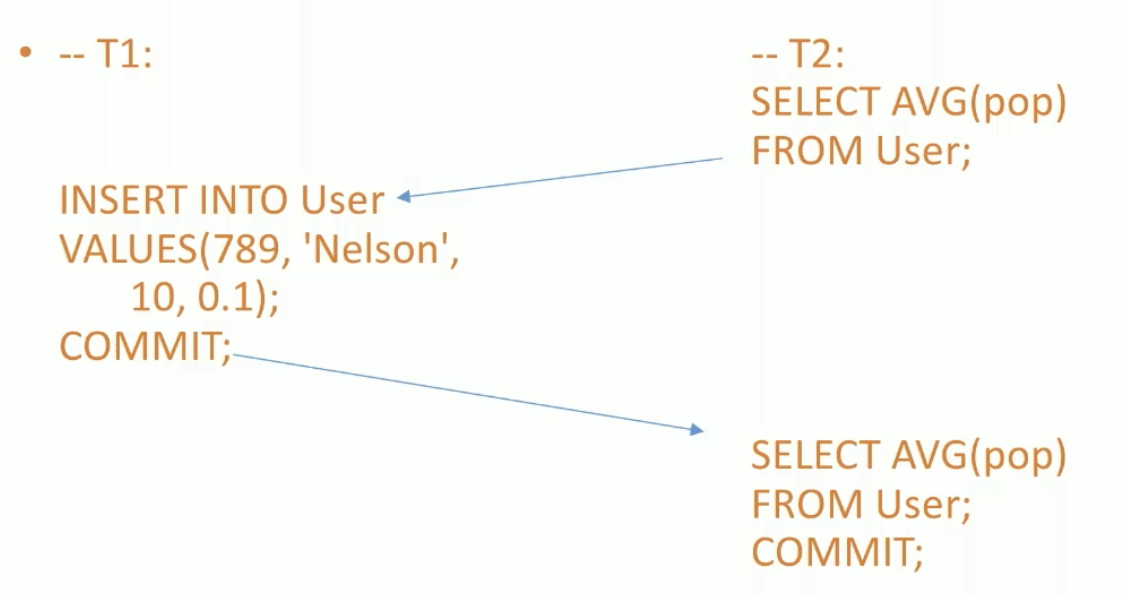
\includegraphics[scale=0.4]{img/rep_read.png}
        \caption{You still have a different average due to the insertion of a new element. } 
        \label{fig:rep_read}
      \end{figure}

      \item \texttt{READ COMMITTED} does not allow dirty reads, but non-repeatable reads are allowed (RW conflicts), which means that reading the same data twice can produce different results and is allowed. 

      \begin{figure}[H]
        \centering 
        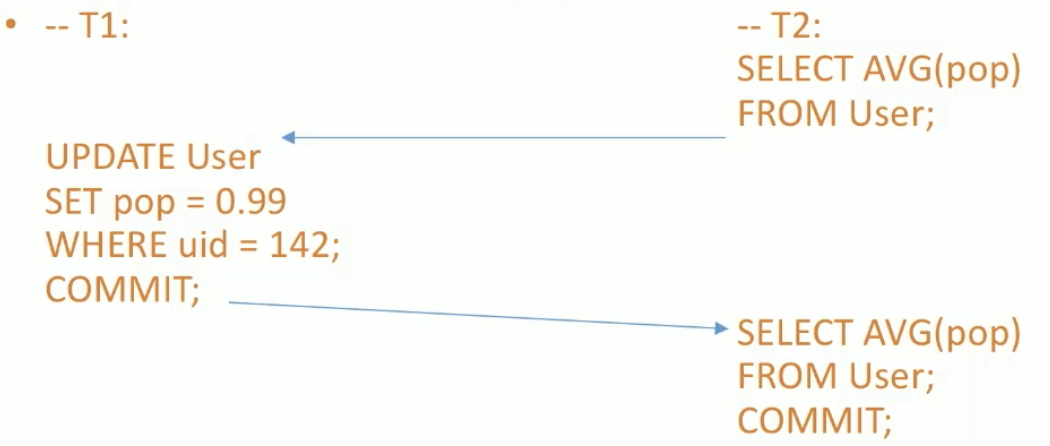
\includegraphics[scale=0.4]{img/read_c.png}
        \caption{In T2, we first compute an average of say 0.6. Then in T1 we update the popularity and commit. Then in T2, we take the average again, getting 0.8, and finally commit. T2 ends up reading two different states of the database.} 
        \label{fig:read_committed}
      \end{figure}

      \item \texttt{READ UNCOMMITTED} allows you to read uncommitted/dirty data (WR conflict). 

      \begin{figure}[H]
        \centering 
        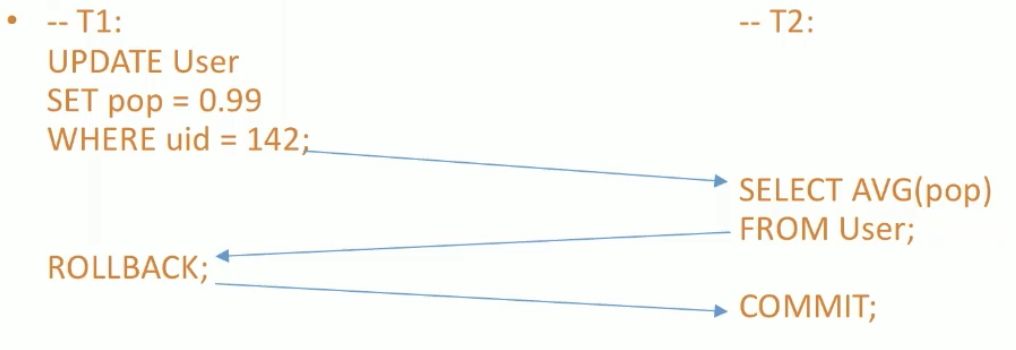
\includegraphics[scale=0.4]{img/read_unc.png}
        \caption{In T1, you are setting the popularity to 0.99. In T2, you read this uncommitted data to compute the average. However, T1 aborts this write, and in T2 you are left with the wrong average. } 
        \label{fig:read_uncommitted}
      \end{figure}
    \end{enumerate}

    Here is a summary of the isolation levels.\footnote{Postgres defaults to read committed.}

    \begin{figure}[H]
      \centering 
      \includegraphics[scale=0.4]{img/isolation.png}
      \caption{} 
      \label{fig:isolation}
    \end{figure}

  \subsection{Serizability and Precedence Graph}

    Okay, so serial schedules are trivial to construct and ideally we want to construct serializable schedules. How do we detect them? We can make a \textbf{precedence graph}. 

\end{document}
